% ============================================================
%  PLANTILLA OFICIAL -- Universidad de Salamanca
%  Grado en Ingeniería Informática
%  Compilar con: lualatex AnexoI_Especificaciones.tex
% ============================================================

% ============================================================
% NOTA ENCODING (2026-03-27): Archivo corregido a UTF-8.
% Los caracteres acentuados (tildes) habian sido danados por
% una operacion de I/O con codificacion ISO-8859-1 en PS5.
% Patron 1 (AnexoI): U+FFFD para a/e/i/n/u; '?' para 'o'.
%   Solucion: diccionario de contexto + regex (fix_accents_v2.py, fix3.py).
% Patron 2 (AnexoII-V): todos los acentos como '?' literal.
%   Solucion: vacabulario de 462 entradas (fix_annexes_all.py, fix_final.py).
% REGLA: Siempre usar Python 3 + io.open(path,'w',encoding='utf-8').
%        NUNCA usar Set-Content de PowerShell 5 (anade BOM o rompe tildes).
% ============================================================
\documentclass[11pt, a4paper]{article}

% ============================================================
% 1. PAQUETES Y CONFIGURACIÓN GENERAL
% ============================================================

\usepackage{fontspec}
\usepackage[spanish]{babel}
\usepackage{graphicx}
\usepackage{float}
\usepackage{amsmath}
\usepackage{xcolor}
\usepackage[protrusion=true,expansion=false]{microtype}
\usepackage{longtable}
\usepackage{enumitem}
\setlist[enumerate,itemize]{noitemsep, topsep=2pt, parsep=0pt, partopsep=0pt}
\usepackage{array}
\usepackage{booktabs}
\usepackage[
    colorlinks = true,
    linkcolor  = black,
    urlcolor   = black,
    citecolor  = black
]{hyperref}

\usepackage{geometry}
\geometry{
    left       = 2.5cm,
    right      = 2.5cm,
    top        = 3cm,
    bottom     = 2.5cm,
    headheight = 55pt,
    headsep    = 0.8cm
}

\usepackage{pdflscape}
\usepackage{eso-pic}
\usepackage{tikz}
\usetikzlibrary{calc}

\usepackage{listings}
\definecolor{lightgray}{rgb}{0.96, 0.96, 0.96}
\definecolor{darkblue}{rgb}{0.0, 0.0, 0.6}
\definecolor{darkorange}{rgb}{0.8, 0.4, 0.0}

\lstset{
    basicstyle      = \ttfamily\scriptsize,
    breaklines      = true,
    frame           = single,
    backgroundcolor = \color{lightgray},
    keywordstyle    = \color{darkblue}\bfseries,
    stringstyle     = \color{darkorange},
    showstringspaces= false,
}

% ============================================================
% 2. ENCABEZADO Y PIE DE PÁGINA
% ============================================================
\usepackage{fancyhdr}
\pagestyle{fancy}
\fancyhf{}

\lhead{
\includegraphics[height=1.25cm]{USAL-Logo-3820702873.png}}
\rhead{\shortstack[r]{\fontsize{10}{12}\selectfont\textbf{\tituloInforme}\\[-1pt]\fontsize{10}{12}\selectfont\subtituloInforme}}

\renewcommand{\headrulewidth}{0pt}
\renewcommand{\footrulewidth}{0pt}

\cfoot{%
    \color{gray}\rule[0.5ex]{0.4\textwidth}{0.8pt}%
    \hspace{0.5cm}%
    \textcolor{black}{\textbf{\thepage}}%
    \hspace{0.5cm}%
    \color{gray}\rule[0.5ex]{0.4\textwidth}{0.8pt}%
}


% ============================================================
% SOPORTE ENCABEZADO/PIE EN PÁGINAS APAISADAS (landscape)
% ============================================================
\newif\iflscape\lscapefalse

\let\origlandscape\landscape
\let\origendlandscape\endlandscape
\renewenvironment{landscape}{%
  \origlandscape\lscapetrue\thispagestyle{empty}%
}{%
  \origendlandscape\lscapefalse%
}

\AddToShipoutPictureFG{%
  \iflscape
    \begin{tikzpicture}[remember picture, overlay]
      % pdflscape rota CW para visualización:
      % lado IZQUIERDO físico (west) = ARRIBA del apaisado → encabezado
                        % Cabecera con logo y texto apilado en la banda de encabezado (west = arriba)
      \node[rotate=90, anchor=center, inner sep=0pt]
        at ([xshift=1.0cm]current page.west)
        {\makebox[\textheight]{%
                                        
\includegraphics[height=1.1cm]{USAL-Logo-3820702873.png}\hfill%
                                        \shortstack[r]{\fontsize{10}{12}\selectfont\textbf{\tituloInforme}\\[-1pt]\fontsize{10}{12}\selectfont\subtituloInforme}}};
      % lado DERECHO físico (east) = ABAJO del apaisado → número de página
      \node[rotate=90, anchor=center, inner sep=0pt]
        at ([xshift=-1.5cm]current page.east)
        {\color{gray}\rule[0.5ex]{5cm}{0.8pt}%
         \hspace{0.4cm}\textcolor{black}{\textbf{\thepage}}\hspace{0.4cm}%
         \color{gray}\rule[0.5ex]{5cm}{0.8pt}};
    \end{tikzpicture}%
  \fi%
}

% ============================================================
% 3. DATOS DEL INFORME
% ============================================================

\newcommand{\tituloInforme}{Anexo I: Especificaciones del sistema}
\newcommand{\subtituloInforme}{Sistema de Gestión Documental mediante Blockchain}
\newcommand{\asignatura}{Trabajo de Fin de Grado}
\newcommand{\autorUno}{David Pérez Velasco}
\newcommand{\tutorUno}{Gabriel Villarrubia González}
\newcommand{\tutorDos}{Sergio García González}

% ============================================================
% 4. DOCUMENTO
% ============================================================
\graphicspath{{diagramas/}}
\begin{document}

% ------------------------------------------------------------
% PORTADA
% ------------------------------------------------------------
\begin{titlepage}
    \centering
    \vspace*{1.5cm}

    {\scshape\LARGE Universidad de Salamanca \par}
    \vspace{1cm}
    {\scshape\Large Grado en Ingeniería Informática \par}
    \vspace{1.5cm}

    {\huge\bfseries \tituloInforme \par}
    \vspace{0.5cm}
    {\Large\bfseries \subtituloInforme \par}
    \vspace{1.8cm}

    
\includegraphics[width=0.34\textwidth]{USAL-Logo-3820702873.png}

    \vspace{1.8cm}

    {\Large\itshape \autorUno \par}
    \vspace{2cm}
    
    {\large Tutores: \par}
    \vspace{0.3cm}
    {\large \tutorUno \par}
    \vspace{0.2cm}
    {\large \tutorDos \par}

    \vfill

    \asignatura

    \vspace{1cm}
\end{titlepage}

\setcounter{page}{2}
\pagestyle{fancy}

% ------------------------------------------------------------
% ÍNDICE
% ------------------------------------------------------------
\tableofcontents
\newpage

\listoffigures
\newpage

\listoftables
\newpage

% ============================================================
% CONTENIDO DEL ANEXO I
% ============================================================

\section{Introducción}

Este anexo recoge la especificación completa de requisitos del sistema \textbf{DocumentChain}, un sistema de gestión documental descentralizado basado en tecnología blockchain y almacenamiento distribuido IPFS. El documento sigue la metodología de elicitación de requisitos de \textbf{Durán y Bernárdez}, estableciendo un contrato claro entre el desarrollador, los tutores y el tribunal evaluador.

DocumentChain permite a los usuarios gestionar documentos de forma segura mediante:
\begin{itemize}
    \item Protección criptográfica de documentos privados con AES-256-GCM
    \item Almacenamiento distribuido sobre una capa IPFS compatible
    \item Registro inmutable en blockchain Ethereum
    \item Control de acceso granular mediante smart contracts
    \item Firmas digitales verificables on-chain
    \item Versionado completo de documentos
    \item Gestión multi-wallet para firma de operaciones blockchain
\end{itemize}

La especificación se estructura en tres tipos de requisitos:
\begin{itemize}
    \item \textbf{Requisitos de Información (IRQ)}: Entidades y datos que el sistema debe almacenar
    \item \textbf{Requisitos No Funcionales (NFR)}: Restricciones de calidad, rendimiento y seguridad
    \item \textbf{Requisitos Funcionales (UC)}: Casos de uso y funcionalidades específicas
\end{itemize}

\section{Lista de usuarios participantes}

\subsection{Participante -- David Pérez Velasco}

\begin{table}[H]
    \centering
    \small
    \begin{tabular}{|p{4cm}|p{10cm}|}
    \hline
    \textbf{Participante} & David Pérez Velasco \\
    \hline
    \textbf{Organización} & Universidad de Salamanca \\
    \hline
    \textbf{Rol} & Desarrollador / Alumno \\
    \hline
    \textbf{Es desarrollador} & Sí \\
    \hline
    \textbf{Es cliente} & No \\
    \hline
    \textbf{Es usuario} & Sí \\
    \hline
    \textbf{Comentarios} & Responsable completo del desarrollo del sistema \\
    \hline
    \end{tabular}
    \caption{Participante -- David Pérez Velasco}
\end{table}

\subsection{Participante -- Gabriel Villarrubia González}

\begin{table}[H]
    \centering
    \small
    \begin{tabular}{|p{4cm}|p{10cm}|}
    \hline
    \textbf{Participante} & Gabriel Villarrubia González \\
    \hline
    \textbf{Organización} & Universidad de Salamanca \\
    \hline
    \textbf{Rol} & Tutor / Director \\
    \hline
    \textbf{Es desarrollador} & No \\
    \hline
    \textbf{Es cliente} & Sí \\
    \hline
    \textbf{Es usuario} & No \\
    \hline
    \textbf{Comentarios} & Supervisión técnica y validación de requisitos \\
    \hline
    \end{tabular}
    \caption{Participante -- Gabriel Villarrubia González}
\end{table}

\subsection{Participante -- Sergio García González}

\begin{table}[H]
    \centering
    \small
    \begin{tabular}{|p{4cm}|p{10cm}|}
    \hline
    \textbf{Participante} & Sergio García González \\
    \hline
    \textbf{Organización} & Universidad de Salamanca \\
    \hline
    \textbf{Rol} & Tutor / Director \\
    \hline
    \textbf{Es desarrollador} & No \\
    \hline
    \textbf{Es cliente} & Sí \\
    \hline
    \textbf{Es usuario} & No \\
    \hline
    \textbf{Comentarios} & Supervisión técnica y validación de requisitos \\
    \hline
    \end{tabular}
    \caption{Participante -- Sergio García González}
\end{table}

\section{Objetivos del proyecto}

\subsection{OBJ-0001: Gestionar usuarios y seguridad}

\begin{table}[H]
    \centering
    \small
    \begin{tabular}{|p{4cm}|p{10cm}|}
    \hline
    \textbf{OBJ-0001} & Gestionar usuarios y seguridad \\
    \hline
    \textbf{Versión} & 1.0 \\
    \hline
    \textbf{Autores} & David Pérez Velasco \\
    \hline
    \textbf{Fuentes} & A. Durán, B. Bernárdez \\
    \hline
    \textbf{Descripción} & El sistema debe proporcionar un módulo completo de gestión de usuarios con autenticación robusta mediante JWT y verificación de firmas de wallet (EIP-191). Debe soportar méltiples wallets por usuario (máximo 5), autenticación de dos factores (2FA), recuperación de contraseña, y gestión de perfiles. Los roles de usuario (USER, ADMIN) determinarán el acceso a funcionalidades administrativas. \\
    \hline
    \textbf{Subobjetivos} & Ninguno \\
    \hline
    \textbf{Importancia} & Vital \\
    \hline
    \textbf{Estado} & Completado \\
    \hline
    \textbf{Estabilidad} & Alta \\
    \hline
    \textbf{Comentarios} & Crítico para la seguridad del sistema completo \\
    \hline
    \end{tabular}
    \caption{Especificación del objetivo OBJ-0001}
\end{table}

\subsection{OBJ-0002: Integración blockchain y almacenamiento descentralizado}

\begin{table}[H]
    \centering
    \small
    \begin{tabular}{|p{4cm}|p{10cm}|}
    \hline
    \textbf{OBJ-0002} & Integración blockchain y almacenamiento descentralizado \\
    \hline
    \textbf{Versión} & 1.0 \\
    \hline
    \textbf{Autores} & David Pérez Velasco \\
    \hline
    \textbf{Fuentes} & A. Durán, B. Bernárdez \\
    \hline
    \textbf{Descripción} & Integrar un smart contract de Ethereum con OpenZeppelin para registro inmutable de documentos, control de acceso basado en roles y eventos on-chain. Incorporar una capa de almacenamiento IPFS compatible, desplegable sobre proveedor gestionado o clúster propio según el entorno. Sincronizar eventos blockchain con base de datos PostgreSQL mediante event listeners. \\
    \hline
    \textbf{Subobjetivos} & Ninguno \\
    \hline
    \textbf{Importancia} & Vital \\
    \hline
    \textbf{Estado} & Completado \\
    \hline
    \textbf{Estabilidad} & Alta \\
    \hline
    \textbf{Comentarios} & Core del sistema descentralizado \\
    \hline
    \end{tabular}
    \caption{Especificación del objetivo OBJ-0002}
\end{table}

\subsection{OBJ-0003: Protección criptográfica y gestión de claves}

\begin{table}[H]
    \centering
    \small
    \begin{tabular}{|p{4cm}|p{10cm}|}
    \hline
    \textbf{OBJ-0003} & Protección criptográfica y gestión de claves \\
    \hline
    \textbf{Versión} & 1.0 \\
    \hline
    \textbf{Autores} & David Pérez Velasco \\
    \hline
    \textbf{Fuentes} & A. Durán, B. Bernárdez \\
    \hline
    \textbf{Descripción} & Implementar protección criptográfica para documentos privados mediante AES-256-GCM y claves simétricas específicas por documento o versión. Utilizar pares RSA-OAEP de 4096 bits para proteger esas claves simétricas durante descargas, comparticiones y transferencias privadas. Conservar las contraseñas con Argon2id y cifrar la clave privada del usuario con AES-256-GCM derivando material criptográfico desde la contraseña o desde la clave de recuperación, según el flujo. Contemplar además la publicación explícita de documentos públicos mediante identificador compartible, enlace y código QR. \\
    \hline
    \textbf{Subobjetivos} & Ninguno \\
    \hline
    \textbf{Importancia} & Vital \\
    \hline
    \textbf{Estado} & Completado \\
    \hline
    \textbf{Estabilidad} & Alta \\
    \hline
    \textbf{Comentarios} & La privacidad se aplica por defecto a los documentos privados; la publicación pública requiere activación explícita y cambia deliberadamente el modelo de acceso. \\
    \hline
    \end{tabular}
    \caption{Especificación del objetivo OBJ-0003}
\end{table}

\subsection{OBJ-0004: Versionado y trazabilidad completa}

\begin{table}[H]
    \centering
    \small
    \begin{tabular}{|p{4cm}|p{10cm}|}
    \hline
    \textbf{OBJ-0004} & Versionado y trazabilidad completa \\
    \hline
    \textbf{Versión} & 1.0 \\
    \hline
    \textbf{Autores} & David Pérez Velasco \\
    \hline
    \textbf{Fuentes} & A. Durán, B. Bernárdez \\
    \hline
    \textbf{Descripción} & Permitir méltiples versiones por documento con seguimiento completo en blockchain. Implementar versión operativa (activa) y capacidad de restaurar versiones antiguas. Registrar timeline completo de eventos (creación, modificación, firma, compartir, transferencia). Mantener estadísticas detalladas por documento y usuario. \\
    \hline
    \textbf{Subobjetivos} & Ninguno \\
    \hline
    \textbf{Importancia} & Alta \\
    \hline
    \textbf{Estado} & Completado \\
    \hline
    \textbf{Estabilidad} & Alta \\
    \hline
    \textbf{Comentarios} & Esencial para auditoría y compliance \\
    \hline
    \end{tabular}
    \caption{Especificación del objetivo OBJ-0004}
\end{table}

\subsection{OBJ-0005: Firmas digitales verificables}

\begin{table}[H]
    \centering
    \small
    \begin{tabular}{|p{4cm}|p{10cm}|}
    \hline
    \textbf{OBJ-0005} & Firmas digitales verificables \\
    \hline
    \textbf{Versión} & 1.0 \\
    \hline
    \textbf{Autores} & David Pérez Velasco \\
    \hline
    \textbf{Fuentes} & A. Durán, B. Bernárdez \\
    \hline
    \textbf{Descripción} & Implementar sistema de firmas digitales on-chain donde cualquier usuario con acceso a un documento puede firmarlo mediante su wallet. Las firmas se registran en el smart contract con timestamp blockchain. Permitir comentarios en firmas y verificación de autenticidad. \\
    \hline
    \textbf{Subobjetivos} & Ninguno \\
    \hline
    \textbf{Importancia} & Alta \\
    \hline
    \textbf{Estado} & Completado \\
    \hline
    \textbf{Estabilidad} & Alta \\
    \hline
    \textbf{Comentarios} & Proporciona no repudio y validez legal \\
    \hline
    \end{tabular}
    \caption{Especificación del objetivo OBJ-0005}
\end{table}

\subsection{OBJ-0006: Control de acceso granular}

\begin{table}[H]
    \centering
    \small
    \begin{tabular}{|p{4cm}|p{10cm}|}
    \hline
    \textbf{OBJ-0006} & Control de acceso granular \\
    \hline
    \textbf{Versión} & 1.0 \\
    \hline
    \textbf{Autores} & David Pérez Velasco \\
    \hline
    \textbf{Fuentes} & A. Durán, B. Bernárdez \\
    \hline
    \textbf{Descripción} & Implementar sistema de permisos con roles: OWNER (control total), EDITOR (lectura y escritura), VIEWER (solo lectura) y NONE (sin acceso). Los permisos vigentes se consultan on-chain y el backend conserva la proyección operativa necesaria para la interfaz, la trazabilidad y las notificaciones. Debe permitirse la revocación de acceso y la transferencia de propiedad. \\
    \hline
    \textbf{Subobjetivos} & Ninguno \\
    \hline
    \textbf{Importancia} & Alta \\
    \hline
    \textbf{Estado} & Completado \\
    \hline
    \textbf{Estabilidad} & Alta \\
    \hline
    \textbf{Comentarios} & Flexible para colaboración multi-usuario \\
    \hline
    \end{tabular}
    \caption{Especificación del objetivo OBJ-0006}
\end{table}

\section{Catálogo de requisitos del sistema}

\subsection{Requisitos de información}

\subsubsection{IRQ-0001: Datos de usuario y autenticación}

\begin{table}[H]
    \centering
    \small
    \begin{tabular}{|p{4cm}|p{10cm}|}
    \hline
    \textbf{IRQ-0001} & Datos de usuario y autenticación \\
    \hline
    \textbf{Versión} & 1.0 \\
    \hline
    \textbf{Autores} & David Pérez Velasco \\
    \hline
    \textbf{Fuentes} & A. Durán, B. Bernárdez \\
    \hline
    \textbf{Descripción} & Información completa de usuarios del sistema incluyendo credenciales, perfiles, y wallets blockchain asociadas. \\
    \hline
    \textbf{Datos específicos} & 
    \textbf{Usuario:}
    \begin{itemize}
        \item ID único, Username, Email (únicos)
        \item Password hash, Nombre completo, Rol (USER/ADMIN)
        \item Par de claves criptográficas (pública/privada encriptada)
        \item Clave de recuperación, 2FA (secret, códigos backup)
        \item Estado de suspensión (boolean + motivo)
        \item Timestamps (creación, actualización)
    \end{itemize}
    
    \textbf{Wallet:}
    \begin{itemize}
        \item ID único
        \item Dirección de wallet (checksum)
        \item Es primaria (boolean)
        \item Está conectada (boolean)
        \item Alias/nickname
        \item Fecha de añadido
        \item Último uso
    \end{itemize}
    
    \textbf{Sesión:}
    \begin{itemize}
        \item ID único
        \item Access token (JWT)
        \item Refresh token (único)
        \item Fecha de expiración de tokens
        \item Timestamp de creación
        \item Timestamp de éltimo uso
    \end{itemize} \\
    \hline
    \textbf{Importancia} & Vital \\
    \hline
    \textbf{Estado} & Completado \\
    \hline
    \textbf{Estabilidad} & Alta \\
    \hline
    \textbf{Comentarios} & Máximo 5 wallets por usuario. Soporte para autenticación tradicional y wallet. \\
    \hline
    \end{tabular}
    \caption{Especificación del requisito IRQ-0001}
\end{table}

\subsubsection{IRQ-0002: Documentos y versionado}

\begin{table}[H]
    \centering
    \small
    \begin{tabular}{|p{4cm}|p{10cm}|}
    \hline
    \textbf{IRQ-0002} & Documentos y versionado \\
    \hline
    \textbf{Versión} & 1.0 \\
    \hline
    \textbf{Autores} & David Pérez Velasco \\
    \hline
    \textbf{Fuentes} & A. Durán, B. Bernárdez \\
    \hline
    \textbf{Descripción} & Información de documentos almacenados con metadatos, versiones y referencias criptográficas. \\
    \hline
    \textbf{Datos específicos} & 
    \textbf{Documento:}
    \begin{itemize}
        \item ID único, Blockchain ID, Nombre, Descripción
        \item Tipo MIME, Tamaño, Hash de contenido, Extensión
        \item Carpeta (FK), Categoría (FK), Tags, Propietario (FK)
        \item Clave simétrica encriptada, IV y Auth tag de cifrado
        \item Estado blockchain (PREPARING/TX\_SUBMITTED/SYNCED/FAILED), TxHash
        \item Archivado (boolean), Timestamps (creación)
    \end{itemize}
    
    \textbf{Versión:}
    \begin{itemize}
        \item ID único, Documento (FK), Usuario creador (FK)
        \item Número de versión, CID de IPFS
        \item Clave simétrica encriptada, IV, Auth tag
        \item Comentario, Es operativa (activa), Estado blockchain, TxHash
    \end{itemize} \\
    \hline
    \textbf{Importancia} & Vital \\
    \hline
    \textbf{Estado} & Completado \\
    \hline
    \textbf{Estabilidad} & Alta \\
    \hline
    \textbf{Comentarios} & Soporta versionado ilimitado. Solo una versión operativa a la vez. \\
    \hline
    \end{tabular}
    \caption{Especificación del requisito IRQ-0002}
\end{table}

\subsubsection{IRQ-0003: Organización y categorización}

\begin{table}[H]
    \centering
    \small
    \begin{tabular}{|p{4cm}|p{10cm}|}
    \hline
    \textbf{IRQ-0003} & Organización y categorización \\
    \hline
    \textbf{Versión} & 1.0 \\
    \hline
    \textbf{Autores} & David Pérez Velasco \\
    \hline
    \textbf{Fuentes} & A. Durán, B. Bernárdez \\
    \hline
    \textbf{Descripción} & Estructuras para organizar documentos mediante carpetas jerárquicas y categorías. \\
    \hline
    \textbf{Datos específicos} & 
    \textbf{Carpeta:}
    \begin{itemize}
        \item ID único
        \item ID de usuario (FK)
        \item Nombre
        \item Descripción
        \item ID de carpeta padre (FK, nullable)
        \item Color (hex)
        \item Icono
        \item Es compartida (boolean)
        \item Timestamps (creación, actualización)
    \end{itemize}
    
    \textbf{Categoría:}
    \begin{itemize}
        \item ID único
        \item ID de usuario (FK, nullable para predefinidas)
        \item Nombre
        \item Descripción
        \item Color (hex)
        \item Icono
        \item Es predefinida (boolean)
        \item Está activa (boolean)
        \item Timestamp de creación
    \end{itemize} \\
    \hline
    \textbf{Importancia} & Alta \\
    \hline
    \textbf{Estado} & Completado \\
    \hline
    \textbf{Estabilidad} & Alta \\
    \hline
    \textbf{Comentarios} & Carpetas soportan jerarquéa multinivel. Categorías pueden ser del sistema o del usuario. \\
    \hline
    \end{tabular}
    \caption{Especificación del requisito IRQ-0003}
\end{table}

\subsubsection{IRQ-0004: Firmas digitales}

\begin{table}[H]
    \centering
    \small
    \begin{tabular}{|p{4cm}|p{10cm}|}
    \hline
    \textbf{IRQ-0004} & Firmas digitales \\
    \hline
    \textbf{Versión} & 1.0 \\
    \hline
    \textbf{Autores} & David Pérez Velasco \\
    \hline
    \textbf{Fuentes} & A. Durán, B. Bernárdez \\
    \hline
    \textbf{Descripción} & Registro de firmas digitales on-chain con metadata adicional. \\
    \hline
    \textbf{Datos específicos} & 
    \textbf{Firma de Documento:}
    \begin{itemize}
        \item ID único
        \item ID de documento (FK)
        \item ID de versión (FK)
        \item ID de usuario firmante (FK)
        \item ID de wallet firmante (FK)
        \item Timestamp de firma
        \item Estado blockchain
        \item TxHash blockchain
        \item Error blockchain (si aplica)
        \item Reintentos (contador)
    \end{itemize} \\
    \hline
    \textbf{Importancia} & Alta \\
    \hline
    \textbf{Estado} & Completado \\
    \hline
    \textbf{Estabilidad} & Alta \\
    \hline
    \textbf{Comentarios} & Una firma por versión por usuario. Inmutable una vez registrada en blockchain. \\
    \hline
    \end{tabular}
    \caption{Especificación del requisito IRQ-0004}
\end{table}

\subsubsection{IRQ-0005: Eventos y auditoría}

\begin{table}[H]
    \centering
    \small
    \begin{tabular}{|p{4cm}|p{10cm}|}
    \hline
    \textbf{IRQ-0005} & Eventos y auditoría \\
    \hline
    \textbf{Versión} & 1.0 \\
    \hline
    \textbf{Autores} & David Pérez Velasco \\
    \hline
    \textbf{Fuentes} & A. Durán, B. Bernárdez \\
    \hline
    \textbf{Descripción} & Registro completo de todos los eventos del sistema sincronizados desde blockchain. \\
    \hline
    \textbf{Datos específicos} & 
    \textbf{Evento:}
    \begin{itemize}
        \item ID único
        \item Tipo de evento (DocumentCreated, VersionCreated, Signed, etc.)
        \item ID de usuario (FK)
        \item ID de documento (FK, nullable)
        \item Metadata JSON (datos adicionales)
        \item Transaction hash
        \item Número de bloque
        \item Timestamp del bloque
        \item Gas usado
        \item Timestamp de registro local
    \end{itemize} \\
    \hline
    \textbf{Importancia} & Alta \\
    \hline
    \textbf{Estado} & Completado \\
    \hline
    \textbf{Estabilidad} & Alta \\
    \hline
    \textbf{Comentarios} & Permite auditoría completa y timeline de documentos. Sincronizado con blockchain. \\
    \hline
    \end{tabular}
    \caption{Especificación del requisito IRQ-0005}
\end{table}

\subsubsection{IRQ-0006: Estadísticas y métricas}

\begin{table}[H]
    \centering
    \small
    \begin{tabular}{|p{4cm}|p{10cm}|}
    \hline
    \textbf{IRQ-0006} & Estadísticas y métricas \\
    \hline
    \textbf{Versión} & 1.0 \\
    \hline
    \textbf{Autores} & David Pérez Velasco \\
    \hline
    \textbf{Fuentes} & A. Durán, B. Bernárdez \\
    \hline
    \textbf{Descripción} & Métricas agregadas para usuarios, documentos y sistema global. \\
    \hline
    \textbf{Datos específicos} & 
    \textbf{User Stats:}
    \begin{itemize}
        \item Documentos totales, Tamaño total, Descargas
        \item Compartidos, Firmas, Transferencias, Restauraciones
        \item Última actividad
    \end{itemize}
    
    \textbf{Document Stats:}
    \begin{itemize}
        \item Total versiones
        \item Total firmas
        \item Total descargas
        \item Total compartidos
        \item Total vistas
        \item Total restauraciones
        \item Última actividad
    \end{itemize}
    
    \textbf{System Stats:}
    \begin{itemize}
        \item Tipo (daily/weekly/monthly), Período (inicio-fin)
        \item Usuarios (nuevos, activos, total)
        \item Documentos (nuevos, total), Storage (nuevo, total)
        \item Total eventos, Último bloque sincronizado
    \end{itemize} \\
    \hline
    \textbf{Importancia} & Media \\
    \hline
    \textbf{Estado} & Completado \\
    \hline
    \textbf{Estabilidad} & Alta \\
    \hline
    \textbf{Comentarios} & Optimizado para dashboard de administración. Actualizado incremental. \\
    \hline
    \end{tabular}
    \caption{Especificación del requisito IRQ-0006}
\end{table}

\subsubsection{IRQ-0007: Notificaciones y comunicaciones}

\begin{table}[H]
    \centering
    \small
    \begin{tabular}{|p{4cm}|p{10cm}|}
    \hline
    \textbf{IRQ-0007} & Notificaciones y comunicaciones \\
    \hline
    \textbf{Versión} & 1.0 \\
    \hline
    \textbf{Autores} & David Pérez Velasco \\
    \hline
    \textbf{Fuentes} & A. Durán, B. Bernárdez \\
    \hline
    \textbf{Descripción} & Sistema de notificaciones in-app y por email con preferencias configurables. \\
    \hline
    \textbf{Datos específicos} & 
    \textbf{Notificación:}
    \begin{itemize}
        \item ID único
        \item ID de usuario (FK)
        \item Tipo (document\_shared, version\_created, signature\_added, etc.)
        \item Título
        \item Mensaje
        \item Metadata JSON
        \item Leída (boolean)
        \item Fecha de lectura
        \item Timestamp de creación
    \end{itemize}
    
    \textbf{Preferencias de Notificación:}
    \begin{itemize}
        \item Email para documentos compartidos
        \item Email para nuevas versiones
        \item Email para firmas
        \item Email para transferencias
        \item Notificaciones in-app habilitadas
        \item Email digest (daily, weekly, never)
    \end{itemize}
    
    \textbf{Verificación de Email:}
    \begin{itemize}
        \item Token de verificación
        \item Email a verificar
        \item Fecha de expiración
        \item Verificado (boolean)
    \end{itemize}
    
    \textbf{Recuperación de Contraseña:}
    \begin{itemize}
        \item Token de reset
        \item Fecha de expiración
        \item Usado (boolean)
    \end{itemize} \\
    \hline
    \textbf{Importancia} & Media \\
    \hline
    \textbf{Estado} & Completado \\
    \hline
    \textbf{Estabilidad} & Alta \\
    \hline
    \textbf{Comentarios} & Integrado con sistema de email configurable (SMTP/Sendgrid/MS365). WebSocket para notificaciones en tiempo real. \\
    \hline
    \end{tabular}
    \caption{Especificación del requisito IRQ-0007}
\end{table}

\subsection{Requisitos no funcionales}

\subsubsection{NFR-0001: Seguridad y privacidad de datos}

\begin{table}[H]
    \centering
    \small
    \begin{tabular}{|p{4cm}|p{10cm}|}
    \hline
    \textbf{NFR-0001} & Seguridad y privacidad de datos \\
    \hline
    \textbf{Versión} & 1.0 \\
    \hline
    \textbf{Autores} & David Pérez Velasco \\
    \hline
    \textbf{Fuentes} & A. Durán, B. Bernárdez \\
    \hline
    \textbf{Descripción} & Máximos estándares de seguridad para protección de datos sensibles. \\
    \hline
    \textbf{Restricciones} & 
    \begin{enumerate}
        \item Cifrado AES-256-GCM para documentos privados; la publicación pública solo puede realizarse de forma explícita y mostrando aviso previo al usuario
        \item Claves privadas nunca enviadas al backend (solo en memoria cliente)
        \item Auto-clear de claves después de 15 minutos de inactividad
        \item HTTPS obligatorio (TLS 1.3)
        \item Argon2id para hashing de contraseñas
        \item JWT con refresh tokens rotativos
        \item CORS configurado restrictivamente
        \item Headers de seguridad HTTP (HSTS, X-Frame-Options, CSP)
        \item Rate limiting en endpoints críticos
        \item Validación estricta de entrada (sanitización)
        \item Protección contra SQL injection, XSS, CSRF
        \item Auditoría completa de accesos
        \item Logs de seguridad encriptados
        \item Backup encriptado de base de datos
    \end{enumerate} \\
    \hline
    \textbf{Importancia} & Vital \\
    \hline
    \textbf{Estado} & Completado \\
    \hline
    \textbf{Estabilidad} & Alta \\
    \hline
    \textbf{Comentarios} & Cumple estándares OWASP Top 10. Los documentos privados se cifran antes de almacenarse de forma persistente y el descifrado operativo para lectura, compartición y transferencia se realiza en el cliente autenticado. \\
    \hline
    \end{tabular}
    \caption{Especificación del requisito NFR-0001}
\end{table}

\subsubsection{NFR-0002: Rendimiento y escalabilidad}

\begin{table}[H]
    \centering
    \small
    \begin{tabular}{|p{4cm}|p{10cm}|}
    \hline
    \textbf{NFR-0002} & Rendimiento y escalabilidad \\
    \hline
    \textbf{Versión} & 1.0 \\
    \hline
    \textbf{Autores} & David Pérez Velasco \\
    \hline
    \textbf{Fuentes} & A. Durán, B. Bernárdez \\
    \hline
    \textbf{Descripción} & El sistema debe mantener rendimiento óptimo bajo carga y escalar horizontalmente. \\
    \hline
    \textbf{Restricciones} & 
    \begin{enumerate}
        \item Tamaño máximo de archivo: 100 MB
        \item Tiempo de respuesta API < 2 segundos (p95)
        \item Upload de documentos < 10 segundos para archivos de 10 MB
        \item Download/desencriptado < 5 segundos para archivos de 10 MB
        \item Concurrencia: mínimo 50 usuarios simultáneos
        \item Backend de almacenamiento IPFS configurable, con soporte para redundancia cuando se despliega en clúster autoalojado
        \item Pool de conexiones PostgreSQL optimizado
        \item índices en campos frecuentemente consultados
        \item Lazy loading y paginación en listados
        \item Compresión gzip en respuestas HTTP
        \item Streaming para uploads/downloads grandes
        \item Event listeners con manejo de backpressure
        \item Reintentos exponenciales para transacciones blockchain
    \end{enumerate} \\
    \hline
    \textbf{Importancia} & Alta \\
    \hline
    \textbf{Estado} & Completado \\
    \hline
    \textbf{Estabilidad} & Alta \\
    \hline
    \textbf{Comentarios} & Arquitectura preparada para escalar horizontalmente con balanceador de carga. \\
    \hline
    \end{tabular}
    \caption{Especificación del requisito NFR-0002}
\end{table}

\subsubsection{NFR-0003: Usabilidad y experiencia de usuario}

\begin{table}[H]
    \centering
    \small
    \begin{tabular}{|p{4cm}|p{10cm}|}
    \hline
    \textbf{NFR-0003} & Usabilidad y experiencia de usuario \\
    \hline
    \textbf{Versión} & 1.0 \\
    \hline
    \textbf{Autores} & David Pérez Velasco \\
    \hline
    \textbf{Fuentes} & A. Durán, B. Bernárdez \\
    \hline
    \textbf{Descripción} & Interfaz intuitiva y responsive con feedback claro al usuario. \\
    \hline
    \textbf{Restricciones} & 
    \begin{enumerate}
        \item Interfaz responsive (mobile-first)
        \item Soporte para navegadores modernos (Chrome, Firefox, Safari, Edge)
        \item Mensajes de error claros y accionables
        \item Loading indicators en operaciones asíncronas
        \item Confirmación para acciones destructivas
        \item Drag \& drop para subida de archivos
        \item Preview de documentos cuando sea posible
        \item Búsqueda y filtrado intuitivos
        \item Shortcuts de teclado para power users
        \item Tema claro/oscuro
        \item Notificaciones toast no intrusivas
        \item Formularios con validación en tiempo real
        \item Accesibilidad WCAG 2.1 nivel AA
    \end{enumerate} \\
    \hline
    \textbf{Importancia} & Alta \\
    \hline
    \textbf{Estado} & Completado \\
    \hline
    \textbf{Estabilidad} & Alta \\
    \hline
    \textbf{Comentarios} & Diseñado con Tailwind CSS y componentes React reutilizables. \\
    \hline
    \end{tabular}
    \caption{Especificación del requisito NFR-0003}
\end{table}

\subsubsection{NFR-0004: Disponibilidad y tolerancia a fallos}

\begin{table}[H]
    \centering
    \small
    \begin{tabular}{|p{4cm}|p{10cm}|}
    \hline
    \textbf{NFR-0004} & Disponibilidad y tolerancia a fallos \\
    \hline
    \textbf{Versión} & 1.0 \\
    \hline
    \textbf{Autores} & David Pérez Velasco \\
    \hline
    \textbf{Fuentes} & A. Durán, B. Bernárdez \\
    \hline
    \textbf{Descripción} & Sistema resiliente con recuperación automática ante fallos. \\
    \hline
    \textbf{Restricciones} & 
    \begin{enumerate}
        \item Disponibilidad objetivo: 99.5\% (permite ~3.6 horas downtime/mes)
        \item Health check endpoint (/api/health)
        \item Logs estructurados con niveles apropiados
        \item Reintentos automáticos para fallos transitorios
        \item Circuit breaker en smart contract (pausable)
        \item Transacciones blockchain con manejo de estados intermedios
        \item Rollback de operaciones fallidas
        \item No se pierden documentos si falla transacción blockchain
        \item Backup diario automatizado de PostgreSQL
        \item Backend de almacenamiento IPFS con replicación o persistencia delegada según el proveedor configurado
        \item Monitoreo de salud de servicios
        \item Manejo graceful de desconexión de red
    \end{enumerate} \\
    \hline
    \textbf{Importancia} & Alta \\
    \hline
    \textbf{Estado} & Completado \\
    \hline
    \textbf{Estabilidad} & Alta \\
    \hline
    \textbf{Comentarios} & Patrón Prepare/Confirm para transacciones blockchain evita inconsistencias. \\
    \hline
    \end{tabular}
    \caption{Especificación del requisito NFR-0004}
\end{table}

\subsubsection{NFR-0005: Mantenibilidad y documentación}

\begin{table}[H]
    \centering
    \small
    \begin{tabular}{|p{4cm}|p{10cm}|}
    \hline
    \textbf{NFR-0005} & Mantenibilidad y documentación \\
    \hline
    \textbf{Versión} & 1.0 \\
    \hline
    \textbf{Autores} & David Pérez Velasco \\
    \hline
    \textbf{Fuentes} & A. Durán, B. Bernárdez \\
    \hline
    \textbf{Descripción} & Código limpio, bien documentado y fácil de mantener. \\
    \hline
    \textbf{Restricciones} & 
    \begin{enumerate}
        \item TypeScript estricto (strict mode)
        \item ESLint y Prettier configurados
        \item Arquitectura en capas (Controllers $\rightarrow$ Services $\rightarrow$ Repositories)
        \item Separación clara de responsabilidades
        \item Código autoexplicativo con nomenclatura clara
        \item Comentarios JSDoc en funciones públicas
        \item Tests unitarios para lógica de negocio crítica
        \item Tests de integración para API
        \item Documentación de API (Swagger/OpenAPI)
        \item README con instrucciones de setup
        \item Variables de entorno documentadas (.env.example)
        \item Git con commits semánticos
        \item Versionado semántico (SemVer)
    \end{enumerate} \\
    \hline
    \textbf{Importancia} & Alta \\
    \hline
    \textbf{Estado} & Completado \\
    \hline
    \textbf{Estabilidad} & Alta \\
    \hline
    \textbf{Comentarios} & Facilita onboarding de nuevos desarrolladores y evolución del sistema. \\
    \hline
    \end{tabular}
    \caption{Especificación del requisito NFR-0005}
\end{table}

\subsubsection{NFR-0006: Portabilidad y despliegue}

\begin{table}[H]
    \centering
    \small
    \begin{tabular}{|p{4cm}|p{10cm}|}
    \hline
    \textbf{NFR-0006} & Portabilidad y despliegue \\
    \hline
    \textbf{Versión} & 1.0 \\
    \hline
    \textbf{Autores} & David Pérez Velasco \\
    \hline
    \textbf{Fuentes} & A. Durán, B. Bernárdez \\
    \hline
    \textbf{Descripción} & Sistema portable y fácil de desplegar en méltiples entornos. \\
    \hline
    \textbf{Restricciones} & 
    \begin{enumerate}
        \item Docker Compose para servicios autoalojados opcionales, incluido IPFS Cluster
        \item Scripts PowerShell para desarrollo Windows
        \item Variables de entorno para configuración
        \item Sin hardcodeo de credenciales
        \item Base de datos PostgreSQL (portable a AWS RDS, Azure, etc.)
        \item Compatible con proveedores blockchain (Infura, Alchemy, nodo propio)
        \item Frontend como SPA (deployable en CDN)
        \item Backend stateless (horizontalmente escalable)
        \item Logs a stdout (compatible con sistemas de logs centralizados)
        \item Scripts de migración de BD versionados (Prisma Migrate)
    \end{enumerate} \\
    \hline
    \textbf{Importancia} & Media \\
    \hline
    \textbf{Estado} & Completado \\
    \hline
    \textbf{Estabilidad} & Alta \\
    \hline
    \textbf{Comentarios} & Preparado para despliegue en cloud (AWS, Azure, GCP) o on-premise. \\
    \hline
    \end{tabular}
    \caption{Especificación del requisito NFR-0006}
\end{table}

\subsection{Requisitos funcionales}

\subsubsection{Diagramas de actores}

\subsubsection{ACT-01: Usuario}

\begin{table}[H]
    \centering
    \small
    \begin{tabular}{|p{4cm}|p{10cm}|}
    \hline
    \textbf{ACT-01} & Usuario \\
    \hline
    \textbf{Versión} & 1.0 \\
    \hline
    \textbf{Autores} & David Pérez Velasco \\
    \hline
    \textbf{Fuentes} & A. Durán, B. Bernárdez \\
    \hline
    \textbf{Descripción} & Usuario estándar del sistema con rol USER. Puede gestionar sus propios documentos, compartir, firmar, crear versiones, y colaborar con otros usuarios. \\
    \hline
    \textbf{Responsabilidades} & 
    \begin{enumerate}
        \item Registrarse y autenticarse en el sistema
        \item Conectar méltiples wallets de Ethereum
        \item Subir y descargar documentos
        \item Crear y gestionar carpetas y categorías
        \item Crear nuevas versiones de documentos
        \item Firmar documentos digitalmente
        \item Compartir documentos con otros usuarios
        \item Gestionar permisos de acceso a sus documentos
        \item Transferir propiedad de documentos
        \item Archivar y restaurar documentos
        \item Ver timeline y estadísticas
        \item Configurar perfil y notificaciones
        \item Activar 2FA para mayor seguridad
    \end{enumerate} \\
    \hline
    \textbf{Comentarios} & Actor principal del sistema. Interactúa con todos los módulos funcionales. \\
    \hline
    \end{tabular}
    \caption{Especificación del actor ACT-01}
\end{table}

\subsubsection{ACT-02: Administrador}

\begin{table}[H]
    \centering
    \small
    \begin{tabular}{|p{4cm}|p{10cm}|}
    \hline
    \textbf{ACT-02} & Administrador \\
    \hline
    \textbf{Versión} & 1.0 \\
    \hline
    \textbf{Autores} & David Pérez Velasco \\
    \hline
    \textbf{Fuentes} & A. Durán, B. Bernárdez \\
    \hline
    \textbf{Descripción} & Usuario con rol ADMIN. Tiene todas las capacidades de un usuario normal más funcionalidades administrativas para supervisión y gestión del sistema. \\
    \hline
    \textbf{Responsabilidades} & 
    \begin{enumerate}
        \item Todas las responsabilidades de Usuario
        \item Ver estadísticas globales del sistema
        \item Listar todos los usuarios
        \item Crear nuevos administradores
        \item Modificar roles de usuarios
        \item Suspender o eliminar usuarios
        \item Ver logs de auditoría completos
        \item Pausar/despausar el smart contract (emergencias)
        \item Sincronizar administradores con blockchain
        \item Ver estado del sistema (salud de servicios)
        \item Acceder al auditor blockchain
    \end{enumerate} \\
    \hline
    \textbf{Comentarios} & Hereda de Usuario. Acceso solo por consola (no auto-registro). \\
    \hline
    \end{tabular}
    \caption{Especificación del actor ACT-02}
\end{table}

\subsubsection{ACT-03: Smart Contract (DocumentRegistry)}

\begin{table}[H]
    \centering
    \small
    \begin{tabular}{|p{4cm}|p{10cm}|}
    \hline
    \textbf{ACT-03} & Smart Contract (DocumentRegistry) \\
    \hline
    \textbf{Versión} & 1.0 \\
    \hline
    \textbf{Autores} & David Pérez Velasco \\
    \hline
    \textbf{Fuentes} & A. Durán, B. Bernárdez \\
    \hline
    \textbf{Descripción} & Contrato inteligente desplegado en Ethereum que mantiene el registro inmutable de documentos, versiones, permisos y firmas. \\
    \hline
    \textbf{Responsabilidades} & 
    \begin{enumerate}
        \item Registrar creación de documentos
        \item Registrar creación de versiones
        \item Gestionar permisos de documentos (OWNER, VIEWER, EDITOR)
        \item Registrar firmas digitales
        \item Validar permisos antes de operaciones
        \item Emitir eventos para sincronización
        \item Permitir transferencias de propiedad
        \item Soportar pausa de emergencia (Pausable)
        \item Control de acceso basado en roles (AccessControl)
        \item Mantener contadores y enumeraciones
    \end{enumerate} \\
    \hline
    \textbf{Comentarios} & Actor no humano. Fuente única de verdad para estado blockchain. \\
    \hline
    \end{tabular}
    \caption{Especificación del actor ACT-03}
\end{table}

\subsubsection{ACT-04: Proveedor IPFS compatible}

\begin{table}[H]
    \centering
    \small
    \begin{tabular}{|p{4cm}|p{10cm}|}
    \hline
    \textbf{ACT-04} & Proveedor IPFS compatible \\
    \hline
    \textbf{Versión} & 1.0 \\
    \hline
    \textbf{Autores} & David Pérez Velasco \\
    \hline
    \textbf{Fuentes} & A. Durán, B. Bernárdez \\
    \hline
    \textbf{Descripción} & Servicio de almacenamiento IPFS compatible, desplegable sobre Pinata u otro backend gestionado, o bien sobre un clúster IPFS autoalojado cuando se requiere control directo de la infraestructura. \\
    \hline
    \textbf{Responsabilidades} & 
    \begin{enumerate}
        \item Almacenar archivos cifrados o públicos según la política de visibilidad
        \item Generar CID (Content Identifier) único por archivo
        \item Mantener persistencia del contenido en el backend configurado
        \item Pinning automático o persistencia equivalente del contenido
        \item Unpinning al eliminar documentos
        \item Servir contenido mediante HTTP Gateway
        \item Mantener alta disponibilidad del contenido
    \end{enumerate} \\
    \hline
    \textbf{Comentarios} & Actor no humano. Backend interactúa vía API HTTP del cluster. \\
    \hline
    \end{tabular}
    \caption{Especificación del actor ACT-04}
\end{table}

\subsubsection{ACT-05: Sistema de Email}

\begin{table}[H]
    \centering
    \small
    \begin{tabular}{|p{4cm}|p{10cm}|}
    \hline
    \textbf{ACT-05} & Sistema de Email \\
    \hline
    \textbf{Versión} & 1.0 \\
    \hline
    \textbf{Autores} & David Pérez Velasco \\
    \hline
    \textbf{Fuentes} & A. Durán, B. Bernárdez \\
    \hline
    \textbf{Descripción} & Servicio externo de envío de emails configurado via SMTP, Sendgrid o Microsoft 365. \\
    \hline
    \textbf{Responsabilidades} & 
    \begin{enumerate}
        \item Enviar emails de verificación de cuenta
        \item Enviar emails de recuperación de contraseña
        \item Enviar notificaciones de documentos compartidos
        \item Enviar notificaciones de nuevas versiones
        \item Enviar notificaciones de firmas
        \item Enviar digest periódico de actividad (opcional)
    \end{enumerate} \\
    \hline
    \textbf{Comentarios} & Actor externo. Sistema de fallback: email mock en desarrollo. \\
    \hline
    \end{tabular}
    \caption{Especificación del actor ACT-05}
\end{table}

\subsubsection{Diagramas de casos de uso}

\textbf{NOTA}: Los diagramas se incluirán en formato PlantUML. Ejecutar los archivos .puml separados para generar las imágenes.

% === PlantUML source (comentado) ===
% \begin{lstlisting}[caption={Diagrama general de casos de uso - Ver archivo diagramas/usecase\_general.puml}]
% @startuml
% left to right direction
% skinparam packageStyle rectangle
%
% actor "Usuario" as USER
% actor "Administrador" as ADMIN
% actor "Smart Contract" as SC
% actor "Proveedor IPFS compatible" as IPFS
% actor "Sistema Email" as EMAIL
% actor "Público" as PUB
%
% rectangle "DocumentChain" {
%   package "Gestión de Acceso (01-18)" {
%     usecase "UC-0001: Registrar Usuario" as UC1
%     usecase "UC-0002: Registrar con Wallet" as UC2
%     usecase "UC-0003: Iniciar Sesión" as UC3
%     usecase "UC-0004: Validar Segundo Factor en el Inicio de Sesión" as UC4
%     usecase "UC-0005: Cerrar Sesión" as UC5
%     usecase "UC-0006: Conectar Wallet" as UC6
%     usecase "UC-0007: Eliminar Wallet" as UC7
%     usecase "UC-0008: Wallet Principal" as UC8
%     usecase "UC-0009: Renombrar Wallet" as UC9
%     usecase "UC-0010: Gestionar Perfil" as UC10
%     usecase "UC-0011: Desactivar Cuenta" as UC11
%     usecase "UC-0012: Reactivar Cuenta" as UC12
%     usecase "UC-0013: Cambiar Contraseña" as UC13
%     usecase "UC-0014: Recuperar Contraseña" as UC14
%     usecase "UC-0015: Verificar Email" as UC15
%     usecase "UC-0016: Reenviar Verificación" as UC16
%     usecase "UC-0017: Configurar 2FA" as UC17
%     usecase "UC-0018: Regenerar Backup 2FA" as UC18
%   }
%   package "Gestión de Documentos (19-28)" {
%     usecase "UC-0019: Subir Documento" as UC19
%     usecase "UC-0020: Listar Documentos" as UC20
%     usecase "UC-0021: Ver Detalle" as UC21
%     usecase "UC-0022: Descargar Documento" as UC22
%     usecase "UC-0023: Archivar Documento" as UC23
%     usecase "UC-0024: Desarchivar Documento" as UC24
%     usecase "UC-0025: Eliminar Documento" as UC25
%     usecase "UC-0026: Editar Metadatos" as UC26
%     usecase "UC-0027: Transferir Documento" as UC27
%     usecase "UC-0028: Buscar Documentos" as UC28
%   }
%   package "Versionado (29-33)" {
%     usecase "UC-0029: Crear Nueva Versión" as UC29
%     usecase "UC-0030: Listar Versiones" as UC30
%     usecase "UC-0031: Versión Operativa" as UC31
%     usecase "UC-0032: Restaurar Versión" as UC32
%     usecase "UC-0033: Descargar Versión" as UC33
%   }
%   package "Firmas (34-36)" {
%     usecase "UC-0034: Firmar Documento" as UC34
%     usecase "UC-0035: Ver Firmas" as UC35
%     usecase "UC-0036: Verificar Firma" as UC36
%   }
%   package "Compartición (37-40)" {
%     usecase "UC-0037: Compartir Documento" as UC37
%     usecase "UC-0038: Modificar Permisos" as UC38
%     usecase "UC-0039: Revocar Acceso" as UC39
%     usecase "UC-0040: Docs. Compartidos" as UC40
%   }
%   package "Organización (41-44)" {
%     usecase "UC-0041: Gestionar Carpetas" as UC41
%     usecase "UC-0042: Gestionar Categorías" as UC42
%     usecase "UC-0043: Etiquetar Documento" as UC43
%     usecase "UC-0044: Ver Timeline" as UC44
%   }
%   package "Auditoría y Estadísticas (45-48)" {
%     usecase "UC-0045: Estadísticas Propias" as UC45
%     usecase "UC-0046: Estadísticas Globales" as UC46
%     usecase "UC-0047: Verificar Autenticidad" as UC47
%     usecase "UC-0048: Auditoría Blockchain" as UC48
%   }
%   package "Administración (49-55)" {
%     usecase "UC-0049: Listar Usuarios" as UC49
%     usecase "UC-0050: Gestionar Roles" as UC50
%     usecase "UC-0051: Crear Admin" as UC51
%     usecase "UC-0052: Suspender Usuario" as UC52
%     usecase "UC-0053: Eliminar Cuenta" as UC53
%     usecase "UC-0054: Pausar Sistema" as UC54
%     usecase "UC-0055: Reanudar Sistema" as UC55
%   }
%   package "Notificaciones (56-57)" {
%     usecase "UC-0056: Ver Notificaciones" as UC56
%     usecase "UC-0057: Config. Preferencias" as UC57
%   }
% }
%
% USER --> UC1 ; USER --> UC2 ; USER --> UC3 ; USER --> UC4 ; USER --> UC5
% USER --> UC6 ; USER --> UC7 ; USER --> UC8 ; USER --> UC9 ; USER --> UC10
% USER --> UC11 ; USER --> UC12 ; USER --> UC13 ; USER --> UC14 ; USER --> UC15
% USER --> UC16 ; USER --> UC17 ; USER --> UC18
% USER --> UC19 ; USER --> UC20 ; USER --> UC21 ; USER --> UC22 ; USER --> UC23
% USER --> UC24 ; USER --> UC25 ; USER --> UC26 ; USER --> UC27 ; USER --> UC28
% USER --> UC29 ; USER --> UC30 ; USER --> UC31 ; USER --> UC32 ; USER --> UC33
% USER --> UC34 ; USER --> UC35 ; USER --> UC36
% USER --> UC37 ; USER --> UC38 ; USER --> UC39 ; USER --> UC40
% USER --> UC41 ; USER --> UC42 ; USER --> UC43 ; USER --> UC44
% USER --> UC45 ; USER --> UC56 ; USER --> UC57
% PUB --> UC47
%
% ADMIN --> UC46 ; ADMIN --> UC48
% ADMIN --> UC49 ; ADMIN --> UC50 ; ADMIN --> UC51 ; ADMIN --> UC52
% ADMIN --> UC53 ; ADMIN --> UC54 ; ADMIN --> UC55
%
% UC1 ..> SC : registra ; UC1 ..> EMAIL : envía verificación
% UC2 ..> SC : verifica firma ; UC2 ..> EMAIL : envía verificación
% UC4 ..> SC : verifica desafío
% UC6 ..> SC : verifica firma
% UC19 ..> IPFS : almacena ; UC19 ..> SC : registra
% UC22 ..> IPFS : descarga
% UC27 ..> SC : transferOwnership
% UC29 ..> IPFS : almacena ; UC29 ..> SC : registra
% UC34 ..> SC : registra firma
% UC37 ..> SC : otorga permisos
% UC39 ..> SC : revoca permisos
% UC47 ..> SC : consulta ; UC47 ..> IPFS : verifica
% UC54 ..> SC : pause() ; UC55 ..> SC : unpause()
% @enduml
% \end{lstlisting}
%
% === fin PlantUML ===

\textit{Los diagramas detallados de cada paquete se encuentran en los archivos PlantUML separados en la carpeta diagramas/.}

\textbf{NOTA PARA COMPILACIÓN}: Coloque aquí las imágenes generadas desde PlantUML. Ejemplo:

\begin{figure}[H]
    \centering
    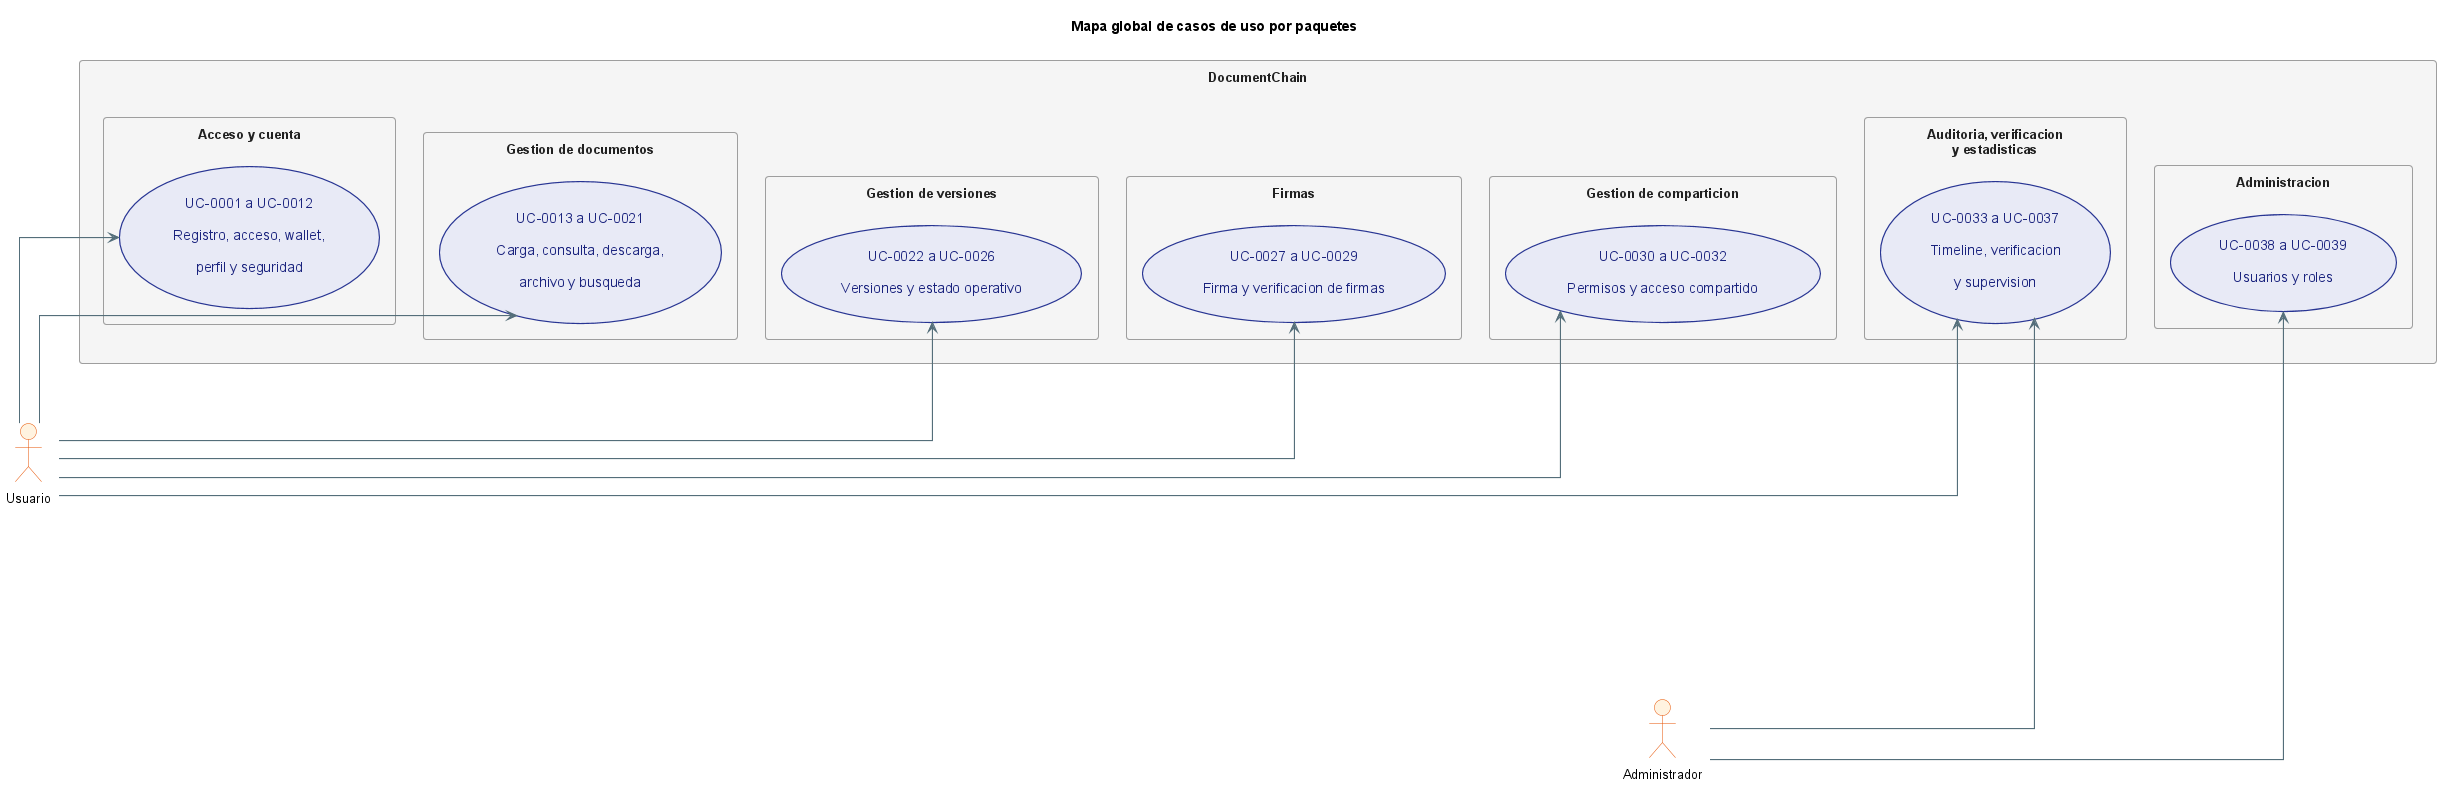
\includegraphics[width=\linewidth]{diagramas/usecase-general.png}
    \caption{Diagrama general de casos de uso del sistema}
    \label{fig:usecase-general}
\end{figure}

\subsubsection{Casos de Uso Detallados}

A continuación se detallan los casos de uso del sistema con un nivel de detalle propio de especificación de requisitos. Cada ficha resume la interacción funcional en entre 4 y 8 pasos, agrupando validaciones técnicas y tareas internas que se desarrollan con mayor profundidad en el Anexo II.

\subsubsection{UC-0001: Registrar Usuario}

\begin{longtable}{|p{4cm}|p{10cm}|}
\hline
\textbf{UC-0001} & Registrar Usuario \\
\hline
\textbf{Versión} & 1.0 \\
\hline
\textbf{Autores} & David Pérez Velasco \\
\hline
\textbf{Fuentes} & A. Durán, B. Bernárdez \\
\hline
\textbf{Descripción} & Permite a un nuevo usuario crear una cuenta en el sistema con generación automática de claves criptográficas. \\
\hline
\textbf{Precondición} & El usuario no debe estar registrado previamente. \\
\hline
\textbf{Secuencia normal} & 
\textbf{Paso 1:} El usuario accede al formulario de registro e introduce sus datos básicos.\newline
\textbf{Paso 2:} El sistema valida que el nombre de usuario, el email y la contraseña cumplen las restricciones definidas.\newline
\textbf{Paso 3:} El backend crea la cuenta y genera el material criptográfico asociado al usuario.\newline
\textbf{Paso 4:} El sistema protege las credenciales sensibles y persiste la información del nuevo usuario.\newline
\textbf{Paso 5:} El sistema genera el proceso de verificación de email y crea la sesión inicial.\newline
\textbf{Paso 6:} El usuario accede a la aplicación con la cuenta recién creada.\\
\hline
\textbf{Postcondición} & Usuario registrado con cuenta activa (sin verificar email inicialmente). \\
\hline
\textbf{Excepciones} & 
\textbf{Paso 2:} Username o email ya existen $\rightarrow$ Error 409 Conflict.\newline
\textbf{Paso 3:} Contraseña débil $\rightarrow$ Error 400 con requisitos.\newline
\textbf{Paso 9:} Fallo al enviar email $\rightarrow$ Continúa pero notifica al usuario.\\
\hline
\textbf{Importancia} & Vital \\
\hline
\textbf{Urgencia} & Inmediata \\
\hline
\textbf{Estado} & Completado \\
\hline
\textbf{Estabilidad} & Alta \\
\hline
\textbf{Comentarios} & Primer punto de entrada al sistema. Proceso completamente automático. \\
\hline
\caption{Especificación del caso de uso UC-0001}
\end{longtable}

\subsubsection{UC-0002: Registrar Usuario y Vincular Wallet Opcionalmente}

\begin{longtable}{|p{4cm}|p{10cm}|}
\hline
\textbf{UC-0002} & Registrar Usuario y Vincular Wallet Opcionalmente \\
\hline
\textbf{Versión} & 1.0 \\
\hline
\textbf{Autores} & David Pérez Velasco \\
\hline
\textbf{Fuentes} & A. Durán, B. Bernárdez \\
\hline
\textbf{Dependencias} & OBJ-0001, OBJ-0003, IRQ-0001, NFR-0001, UC-0006 \\
\hline
\textbf{Descripción} & Permite a un nuevo usuario registrarse con username/email y contraseña, guardar la \textit{Recovery Key} generada por el sistema y, de forma opcional, enlazar una wallet al finalizar el alta para futuras operaciones blockchain. \\
\hline
\textbf{Precondición} & El usuario no está autenticado y dispone de un email válido. La wallet es opcional en este punto y, si se enlaza, no debe estar asociada previamente a otra cuenta. \\
\hline
\textbf{Secuencia normal} & \textbf{Paso 1:} El usuario accede a \texttt{/register} e introduce username, email, contraseña y nombre completo opcional.\newline\textbf{Paso 2:} El frontend envía \texttt{POST /auth/register}.\newline\textbf{Paso 3:} El sistema valida duplicados, genera el material criptográfico del usuario y almacena la cuenta.\newline\textbf{Paso 4:} El sistema genera una \textit{Recovery Key} y la muestra una única vez para que el usuario la guarde.\newline\textbf{Paso 5:} El sistema envía el email de verificación y crea la sesión inicial.\newline\textbf{Paso 6:} El usuario confirma que ha guardado la Recovery Key y entra en la aplicación.\newline\textbf{Paso 7:} De forma opcional, el usuario acepta enlazar una wallet para utilizarla en operaciones blockchain posteriores.\newline\textbf{Paso 8:} Si acepta, el frontend redirige al flujo de conexión de wallet ya autenticado. \\
\hline
\textbf{Postcondición} & Usuario registrado con sesión válida y Recovery Key almacenada por el propio usuario. La wallet puede quedar enlazada opcionalmente, pero no forma parte del mecanismo de autenticación principal. \\
\hline
\textbf{Excepciones} & \textbf{Paso 2:} Username o email duplicado $\rightarrow$ Error 409 Conflict.\newline\textbf{Paso 2:} Contraseña fuera de política $\rightarrow$ Error 400.\newline\textbf{Paso 4:} El usuario no guarda la Recovery Key $\rightarrow$ el frontend bloquea la continuación.\newline\textbf{Paso 7:} Wallet ya asociada a otra cuenta $\rightarrow$ Error 409 Conflict durante el flujo opcional de enlace. \\
\hline
\textbf{Importancia} & Alta \\
\hline
\textbf{Urgencia} & Alta \\
\hline
\textbf{Estado} & Completado \\
\hline
\textbf{Estabilidad} & Alta \\
\hline
\textbf{Comentarios} & En la versión final, el alta se realiza siempre con contraseña. La wallet se añade después del registro para firmar transacciones, no para autenticarse. \\
\hline
\caption{Especificación del caso de uso UC-0002}
\end{longtable}

\subsubsection{UC-0003: Iniciar Sesión}

\begin{longtable}{|p{4cm}|p{10cm}|}
\hline
\textbf{UC-0003} & Iniciar Sesión \\
\hline
\textbf{Versión} & 1.0 \\
\hline
\textbf{Autores} & David Pérez Velasco \\
\hline
\textbf{Fuentes} & A. Durán, B. Bernárdez \\
\hline
\textbf{Dependencias} & OBJ-0001, IRQ-0001, NFR-0001, NFR-0003 \\
\hline
\textbf{Descripción} & Permite a un usuario registrado autenticarse en el sistema mediante credenciales de email o username y contraseña, incorporando un segundo paso de verificación cuando la cuenta tiene 2FA activo. \\
\hline
\textbf{Precondición} & El usuario debe estar registrado en el sistema con cuenta activa (no suspendida). \\
\hline
\textbf{Secuencia normal} &
\textbf{Paso 1:} El usuario accede a \texttt{/login} e introduce username o email y contraseña. \newline
\textbf{Paso 2:} El frontend envía \texttt{POST /auth/login}. \newline
\textbf{Paso 3:} El sistema valida las credenciales y comprueba el estado de la cuenta. \newline
\textbf{Paso 4:} Si el usuario no tiene 2FA activo, el sistema emite JWT y token de refresco. \newline
\textbf{Paso 5:} Si el usuario tiene 2FA activo, el sistema devuelve un token temporal y solicita un segundo factor. \newline
\textbf{Paso 6:} Tras completar la validación correspondiente, el sistema registra la sesión activa y redirige al usuario a \texttt{/app/documents}. \\
\hline
\textbf{Postcondición} & Usuario autenticado con JWT válido. Sesión activa registrada en PostgreSQL. \\
\hline
\textbf{Excepciones} &
\textbf{Paso 3:} Credenciales incorrectas $\rightarrow$ Error 401 ``Credenciales inválidas''. Rate limiting: bloqueo temporal tras 5 intentos en 15 minutos.\newline
\textbf{Paso 3:} Cuenta suspendida $\rightarrow$ Error 403.\newline
\textbf{Paso 5/6:} Código TOTP o código de respaldo incorrecto $\rightarrow$ Error 401.\\
\hline
\textbf{Importancia} & Vital \\
\hline
\textbf{Urgencia} & Inmediata \\
\hline
\textbf{Estado} & Completado \\
\hline
\textbf{Estabilidad} & Alta \\
\hline
\textbf{Comentarios} & El sistema implementa rate limiting para prevenir ataques de fuerza bruta. La wallet queda fuera del proceso de login y se reserva para firmas de operaciones blockchain. \\
\hline
\caption{Especificación del caso de uso UC-0003}
\end{longtable}

\subsubsection{UC-0004: Validar Segundo Factor en el Inicio de Sesión}

\begin{longtable}{|p{4cm}|p{10cm}|}
\hline
\textbf{UC-0004} & Validar Segundo Factor en el Inicio de Sesión \\
\hline
\textbf{Versión} & 1.0 \\
\hline
\textbf{Autores} & David Pérez Velasco \\
\hline
\textbf{Fuentes} & A. Durán, B. Bernárdez \\
\hline
\textbf{Dependencias} & OBJ-0001, IRQ-0001, NFR-0001, UC-0003, UC-0017 \\
\hline
\textbf{Descripción} & Permite completar el proceso de autenticación de una cuenta con 2FA mediante código TOTP o código de respaldo, después de haber validado correctamente usuario y contraseña. \\
\hline
\textbf{Precondición} & El usuario ha superado la validación de credenciales y la cuenta tiene autenticación de dos factores activada. \\
\hline
\textbf{Secuencia normal} & \textbf{Paso 1:} Tras \texttt{POST /auth/login}, el frontend recibe \texttt{requires2FA=true} y un token temporal.\newline\textbf{Paso 2:} El usuario introduce un código TOTP o un código de respaldo.\newline\textbf{Paso 3:} El frontend envía \texttt{POST /auth/2fa/verify-login}.\newline\textbf{Paso 4:} El sistema valida el código frente al secreto TOTP o frente al listado de códigos de respaldo.\newline\textbf{Paso 5:} Si la validación es correcta, el sistema emite JWT, token de refresco y registra la sesión.\newline\textbf{Paso 6:} El usuario es redirigido a la aplicación principal. \\
\hline
\textbf{Postcondición} & Usuario autenticado con JWT válido. Sesión registrada en la base de datos. \\
\hline
\textbf{Excepciones} & \textbf{Paso 4:} Código TOTP inválido $\rightarrow$ Error 401.\newline\textbf{Paso 4:} Código de respaldo ya utilizado o inexistente $\rightarrow$ Error 401.\newline\textbf{Paso 3:} Token temporal expirado $\rightarrow$ Reinicio del proceso de login. \\
\hline
\textbf{Importancia} & Vital \\
\hline
\textbf{Urgencia} & Inmediata \\
\hline
\textbf{Estado} & Completado \\
\hline
\textbf{Estabilidad} & Alta \\
\hline
\textbf{Comentarios} & Este caso de uso sustituye al antiguo acceso con wallet. La autenticación final del sistema combina contraseña y, cuando procede, un segundo factor verificable. \\
\hline
\caption{Especificación del caso de uso UC-0004}
\end{longtable}

\subsubsection{UC-0005: Cerrar Sesión}

\begin{longtable}{|p{4cm}|p{10cm}|}
\hline
\textbf{UC-0005} & Cerrar Sesión \\
\hline
\textbf{Versión} & 1.0 \\
\hline
\textbf{Autores} & David Pérez Velasco \\
\hline
\textbf{Fuentes} & A. Durán, B. Bernárdez \\
\hline
\textbf{Dependencias} & UC-0003, NFR-0001 \\
\hline
\textbf{Descripción} & Permite al usuario finalizar su sesión activa de forma segura, invalidando los tokens de autenticación en el servidor y eliminando las credenciales y claves criptográficas almacenadas en el cliente. \\
\hline
\textbf{Precondición} & El usuario debe tener una sesión activa con JWT válido. \\
\hline
\textbf{Secuencia normal} &
\textbf{Paso 1:} El usuario selecciona ``Cerrar sesión'' en el menú de perfil.\newline
\textbf{Paso 2:} El frontend envía petición con el refresh token.\newline
\textbf{Paso 3:} El backend invalida y elimina el refresh token de la base de datos.\newline
\textbf{Paso 4:} El backend registra el evento de cierre de sesión en los logs del sistema.\newline
\textbf{Paso 5:} El frontend elimina el JWT y el refresh token del almacenamiento local.\newline
\textbf{Paso 6:} El frontend limpia el estado de la aplicación: documentos en caché, clave privada RSA descifrada en RAM y datos de usuario en memoria.\newline
\textbf{Paso 7:} El frontend redirige a la página de inicio de sesión.\\
\hline
\textbf{Postcondición} & Sesión invalidada en el servidor. Tokens eliminados en el cliente. Clave privada RSA descifrada borrada de la memoria RAM. Cualquier petición posterior con el JWT antiguo es rechazada. \\
\hline
\textbf{Excepciones} &
\textbf{Paso 2:} Fallo de red $\rightarrow$ El frontend realiza la limpieza local (pasos 5-7) igualmente para garantizar que el usuario quede desconectado localmente.\newline
\textbf{Paso 3:} Token ya expirado en servidor $\rightarrow$ El backend ignora graciosamente; la limpieza local procede con normalidad.\\
\hline
\textbf{Importancia} & Alta \\
\hline
\textbf{Urgencia} & Inmediata \\
\hline
\textbf{Estado} & Completado \\
\hline
\textbf{Estabilidad} & Alta \\
\hline
\textbf{Comentarios} & La clave privada descifrada solo se mantiene en memoria durante la sesión activa y se elimina al cerrar sesión. El administrador puede cerrar sesiones remotamente desde el panel de administración (UC-0052). \\
\hline
\caption{Especificación del caso de uso UC-0005}
\end{longtable}

\subsubsection{UC-0006: Conectar Wallet}

\begin{longtable}{|p{4cm}|p{10cm}|}
\hline
\textbf{UC-0006} & Conectar Wallet \\
\hline
\textbf{Versión} & 1.0 \\
\hline
\textbf{Autores} & David Pérez Velasco \\
\hline
\textbf{Fuentes} & A. Durán, B. Bernárdez \\
\hline
\textbf{Dependencias} & OBJ-0001, OBJ-0002, IRQ-0001, NFR-0001, UC-0003 \\
\hline
\textbf{Descripción} & Permite al usuario vincular una o varias wallets de Ethereum a su cuenta para utilizarlas en las operaciones que requieren firma sobre blockchain. \\
\hline
\textbf{Precondición} & Usuario autenticado. La dirección a vincular no debe estar asociada previamente a otra cuenta y el usuario no debe haber alcanzado el límite de wallets permitido. \\
\hline
\textbf{Secuencia normal} &
\textbf{Paso 1:} El usuario accede a la gestión de wallets y solicita vincular una nueva dirección. \newline
\textbf{Paso 2:} El sistema ofrece el medio de conexión disponible y el usuario selecciona la wallet que desea asociar. \newline
\textbf{Paso 3:} El sistema solicita una prueba de control sobre esa wallet. \newline
\textbf{Paso 4:} El usuario autoriza la comprobación desde su wallet. \newline
\textbf{Paso 5:} El sistema valida la prueba, registra la wallet y la asocia a la cuenta. \newline
\textbf{Paso 6:} Si es la primera wallet del usuario, queda marcada como principal. \\
\hline
\textbf{Postcondición} & Wallet verificada y asociada a la cuenta del usuario para futuras operaciones firmadas. \\
\hline
\textbf{Excepciones} &
\textbf{Paso 2:} No hay ningún medio de conexión disponible o el usuario cancela la vinculación $\rightarrow$ La operación no continúa.\newline
\textbf{Paso 4:} La prueba de control no resulta válida $\rightarrow$ La wallet no se asocia.\newline
\textbf{Paso 5:} La wallet ya pertenece a otra cuenta o se ha alcanzado el límite permitido $\rightarrow$ El sistema rechaza la vinculación.\\
\hline
\textbf{Importancia} & Alta \\
\hline
\textbf{Urgencia} & Alta \\
\hline
\textbf{Estado} & Completado \\
\hline
\textbf{Estabilidad} & Alta \\
\hline
\textbf{Comentarios} & La wallet vinculada complementa la autenticación principal del sistema y se reserva para operaciones que requieren consentimiento expreso del usuario. \\
\hline
\caption{Especificación del caso de uso UC-0006}
\end{longtable}

\subsubsection{UC-0007: Eliminar Wallet}

\begin{longtable}{|p{4cm}|p{10cm}|}
\hline
\textbf{UC-0007} & Eliminar Wallet \\
\hline
\textbf{Versión} & 1.0 \\
\hline
\textbf{Autores} & David Pérez Velasco \\
\hline
\textbf{Fuentes} & A. Durán, B. Bernárdez \\
\hline
\textbf{Dependencias} & OBJ-0001, IRQ-0001, NFR-0001, UC-0006 \\
\hline
\textbf{Descripción} & Permite al usuario eliminar una wallet previamente asociada a su cuenta. El sistema impide la eliminación si es la única vía de autenticación disponible. \\
\hline
\textbf{Precondición} & Usuario autenticado. El usuario tiene al menos una wallet registrada. \\
\hline
\textbf{Secuencia normal} & \textbf{Paso 1:} El usuario accede a la gestión de wallets y selecciona la dirección que desea eliminar.\newline\textbf{Paso 2:} El sistema comprueba que la eliminación no deja a la cuenta sin un medio válido para operar.\newline\textbf{Paso 3:} El sistema solicita confirmación.\newline\textbf{Paso 4:} El usuario confirma la eliminación.\newline\textbf{Paso 5:} El sistema desvincula la wallet de la cuenta y actualiza la lista mostrada al usuario. \\
\hline
\textbf{Postcondición} & La wallet queda eliminada de la cuenta del usuario y ya no puede usarse para autenticación. \\
\hline
\textbf{Excepciones} & \textbf{Paso 3:} Es la única wallet y no hay otro método de autenticación $\rightarrow$ Error 400 ``No se puede eliminar el único método de autenticación''.\newline\textbf{Paso 3:} La wallet es la principal y es la única $\rightarrow$ Error 400.\newline\textbf{Paso 6:} Wallet no encontrada o no pertenece al usuario $\rightarrow$ Error 404. \\
\hline
\textbf{Importancia} & Media \\
\hline
\textbf{Urgencia} & Media \\
\hline
\textbf{Estado} & Completado \\
\hline
\textbf{Estabilidad} & Alta \\
\hline
\textbf{Comentarios} & Operación reversible a nivel de datos (puede añadirse de nuevo la wallet), pero la sesión activa no se invalida por este cambio. \\
\hline
\caption{Especificación del caso de uso UC-0007}
\end{longtable}

\subsubsection{UC-0008: Establecer Wallet Principal}

\begin{longtable}{|p{4cm}|p{10cm}|}
\hline
\textbf{UC-0008} & Establecer Wallet Principal \\
\hline
\textbf{Versión} & 1.0 \\
\hline
\textbf{Autores} & David Pérez Velasco \\
\hline
\textbf{Fuentes} & A. Durán, B. Bernárdez \\
\hline
\textbf{Dependencias} & OBJ-0001, OBJ-0002, IRQ-0001, NFR-0003, UC-0006 \\
\hline
\textbf{Descripción} & Permite al usuario designar una de sus wallets como la wallet principal utilizada por defecto en las operaciones blockchain (subir documentos, firmar, compartir). \\
\hline
\textbf{Precondición} & Usuario autenticado. El usuario tiene al menos dos wallets registradas o una que aún no es la principal. \\
\hline
\textbf{Secuencia normal} & \textbf{Paso 1:} El usuario accede a la gestión de wallets.\newline\textbf{Paso 2:} Selecciona la wallet que desea utilizar por defecto.\newline\textbf{Paso 3:} El sistema valida que la wallet pertenece al usuario.\newline\textbf{Paso 4:} El sistema actualiza la wallet principal de la cuenta.\newline\textbf{Paso 5:} La interfaz refleja el cambio y la deja preseleccionada para futuras operaciones. \\
\hline
\textbf{Postcondición} & La wallet seleccionada queda marcada como principal. Todas las operaciones blockchain posteriores usarán esta wallet por defecto. \\
\hline
\textbf{Excepciones} & \textbf{Paso 3:} La wallet no pertenece al usuario o no existe $\rightarrow$ El sistema rechaza el cambio.\newline\textbf{Paso 4:} La wallet ya estaba marcada como principal $\rightarrow$ No se producen cambios adicionales. \\
\hline
\textbf{Importancia} & Media \\
\hline
\textbf{Urgencia} & Media \\
\hline
\textbf{Estado} & Completado \\
\hline
\textbf{Estabilidad} & Alta \\
\hline
\textbf{Comentarios} & La wallet principal se propone por defecto cuando el usuario debe firmar una operación, aunque puede cambiarla antes de confirmar. \\
\hline
\caption{Especificación del caso de uso UC-0008}
\end{longtable}

\subsubsection{UC-0009: Renombrar/Etiquetar Wallet}

\begin{longtable}{|p{4cm}|p{10cm}|}
\hline
\textbf{UC-0009} & Renombrar/Etiquetar Wallet \\
\hline
\textbf{Versión} & 1.0 \\
\hline
\textbf{Autores} & David Pérez Velasco \\
\hline
\textbf{Fuentes} & A. Durán, B. Bernárdez \\
\hline
\textbf{Dependencias} & OBJ-0001, IRQ-0001, NFR-0003, UC-0006 \\
\hline
\textbf{Descripción} & Permite al usuario asignar una etiqueta descriptiva a cada wallet para distinguirla con facilidad cuando dispone de varias. \\
\hline
\textbf{Precondición} & Usuario autenticado. El usuario tiene al menos una wallet registrada. \\
\hline
\textbf{Secuencia normal} & \textbf{Paso 1:} El usuario accede a la gestión de wallets y elige la dirección que quiere etiquetar.\newline\textbf{Paso 2:} El sistema muestra la etiqueta actual, si existe.\newline\textbf{Paso 3:} El usuario introduce la nueva denominación y la confirma.\newline\textbf{Paso 4:} El sistema guarda la etiqueta.\newline\textbf{Paso 5:} La interfaz muestra la wallet con la nueva identificación. \\
\hline
\textbf{Postcondición} & La wallet muestra la etiqueta personalizada en todos los contextos de la interfaz. \\
\hline
\textbf{Excepciones} & \textbf{Paso 5:} Etiqueta vacía $\rightarrow$ Se borra la etiqueta existente (operación válida).\newline\textbf{Paso 5:} Etiqueta demasiado larga (>100 caracteres) $\rightarrow$ Error 400. \\
\hline
\textbf{Importancia} & Baja \\
\hline
\textbf{Urgencia} & Baja \\
\hline
\textbf{Estado} & Completado \\
\hline
\textbf{Estabilidad} & Alta \\
\hline
\textbf{Comentarios} & Función de conveniencia especialmente útil para usuarios con múltiples wallets (personal, trabajo, hardware wallet). \\
\hline
\caption{Especificación del caso de uso UC-0009}
\end{longtable}

\subsubsection{UC-0010: Gestionar Perfil}

\begin{longtable}{|p{4cm}|p{10cm}|}
\hline
\textbf{UC-0010} & Gestionar Perfil \\
\hline
\textbf{Versión} & 1.0 \\
\hline
\textbf{Autores} & David Pérez Velasco \\
\hline
\textbf{Fuentes} & A. Durán, B. Bernárdez \\
\hline
\textbf{Dependencias} & OBJ-0001, IRQ-0001, NFR-0003, UC-0003 \\
\hline
\textbf{Descripción} & Permite al usuario autenticado actualizar su información personal: nombre completo, nombre de usuario, dirección de email y foto de perfil (avatar). \\
\hline
\textbf{Precondición} & Usuario autenticado con JWT válido. \\
\hline
\textbf{Secuencia normal} &
\textbf{Paso 1:} El usuario accede a su perfil y consulta los datos actuales.\newline
\textbf{Paso 2:} El usuario modifica los campos permitidos, como nombre, alias, email o avatar.\newline
\textbf{Paso 3:} El sistema valida la unicidad y el formato de la información actualizada.\newline
\textbf{Paso 4:} El backend guarda los cambios en la base de datos.\newline
\textbf{Paso 5:} Si se modifica el email, el sistema reinicia su verificación y envía un nuevo correo de confirmación.\newline
\textbf{Paso 6:} La interfaz confirma que la actualización se ha realizado correctamente.\\
\hline
\textbf{Postcondición} & Información del usuario actualizada en PostgreSQL. Si el email cambi?, se requiere nueva verificación antes de poder usar el email nuevo para login. \\
\hline
\textbf{Excepciones} &
\textbf{Paso 6:} Username ya en uso por otro usuario $\rightarrow$ Error 409 ``Nombre de usuario no disponible''.\newline
\textbf{Paso 7:} Email ya registrado por otro usuario $\rightarrow$ Error 409 ``Email ya registrado en el sistema''.\newline
\textbf{Paso 3:} Avatar con formato no soportado (no PNG/JPG/WEBP) o tamaño $>$2MB $\rightarrow$ Error 400 ``Formato o tamaño inválido''.\\
\hline
\textbf{Importancia} & Media \\
\hline
\textbf{Urgencia} & Media \\
\hline
\textbf{Estado} & Completado \\
\hline
\textbf{Estabilidad} & Alta \\
\hline
\textbf{Comentarios} & El username admite únicamente caracteres alfanuméricos, guiones y guiones bajos. El avatar se redimensiona automáticamente a 200?-200 px en el backend. \\
\hline
\caption{Especificación del caso de uso UC-0010}
\end{longtable}

\subsubsection{UC-0011: Desactivar Propia Cuenta}

\begin{longtable}{|p{4cm}|p{10cm}|}
\hline
\textbf{UC-0011} & Desactivar Propia Cuenta \\
\hline
\textbf{Versión} & 1.0 \\
\hline
\textbf{Autores} & David Pérez Velasco \\
\hline
\textbf{Fuentes} & A. Durán, B. Bernárdez \\
\hline
\textbf{Dependencias} & OBJ-0001, IRQ-0001, NFR-0001 \\
\hline
\textbf{Descripción} & Permite al propio usuario suspender voluntariamente su cuenta, bloqueando el acceso al sistema e invalidando todas sus sesiones activas. La suspensión se propaga también a las wallets en la blockchain. \\
\hline
\textbf{Precondición} & Usuario autenticado con JWT válido. La cuenta no está ya suspendida. \\
\hline
\textbf{Secuencia normal} & \textbf{Paso 1:} El usuario accede al apartado de privacidad y solicita desactivar su cuenta.\newline\textbf{Paso 2:} El sistema muestra una advertencia y solicita confirmación.\newline\textbf{Paso 3:} El usuario confirma la suspensión.\newline\textbf{Paso 4:} El sistema marca la cuenta como suspendida y bloquea su operativa.\newline\textbf{Paso 5:} El sistema invalida las sesiones activas y desconecta al usuario.\newline\textbf{Paso 6:} La suspensión queda reflejada también en la capa blockchain asociada a sus wallets. \\
\hline
\textbf{Postcondición} & Cuenta suspendida y sin sesiones activas válidas. \\
\hline
\textbf{Excepciones} & \textbf{Paso 3:} El usuario cancela la operación $\rightarrow$ La cuenta permanece activa.\newline\textbf{Paso 6:} La propagación a blockchain no puede completarse en ese momento $\rightarrow$ El sistema registra la incidencia para su tratamiento posterior. \\
\hline
\textbf{Importancia} & Media \\
\hline
\textbf{Urgencia} & Baja \\
\hline
\textbf{Estado} & Completado \\
\hline
\textbf{Estabilidad} & Alta \\
\hline
\textbf{Comentarios} & Caso de uso de privacidad y seguridad. Permite al usuario proteger su cuenta inmediatamente si sospecha de un compromiso. La reactivación se realiza mediante UC-0012. \\
\hline
\caption{Especificación del caso de uso UC-0011}
\end{longtable}

\subsubsection{UC-0012: Reactivar Propia Cuenta}

\begin{longtable}{|p{4cm}|p{10cm}|}
\hline
\textbf{UC-0012} & Reactivar Propia Cuenta \\
\hline
\textbf{Versión} & 1.0 \\
\hline
\textbf{Autores} & David Pérez Velasco \\
\hline
\textbf{Fuentes} & A. Durán, B. Bernárdez \\
\hline
\textbf{Dependencias} & OBJ-0001, IRQ-0001, NFR-0001, UC-0011 \\
\hline
\textbf{Descripción} & Permite a un usuario con cuenta suspendida por él mismo (ver UC-0011) reactivarla para recuperar el acceso al sistema. \\
\hline
\textbf{Precondición} & El usuario tiene una cuenta suspendida voluntariamente (no por administrador). El usuario recuerda sus credenciales de acceso. \\
\hline
\textbf{Secuencia normal} & \textbf{Paso 1:} El usuario intenta acceder con sus credenciales habituales.\newline\textbf{Paso 2:} El sistema detecta que la suspensión fue voluntaria y ofrece la reactivación.\newline\textbf{Paso 3:} El usuario solicita recuperar la cuenta y confirma la acción.\newline\textbf{Paso 4:} El sistema reactiva la cuenta y restablece su operativa.\newline\textbf{Paso 5:} El sistema vuelve a habilitar sus wallets asociadas.\newline\textbf{Paso 6:} El usuario recupera el acceso normal a la aplicación. \\
\hline
\textbf{Postcondición} & Cuenta reactivada en base de datos y blockchain. El usuario puede operar normalmente. \\
\hline
\textbf{Excepciones} & \textbf{Paso 2:} La suspensión fue impuesta por un administrador $\rightarrow$ El sistema no muestra la opción de reactivación; solo el admin puede reactivarla.\newline\textbf{Paso 5:} Credenciales inválidas $\rightarrow$ Error 401. \\
\hline
\textbf{Importancia} & Media \\
\hline
\textbf{Urgencia} & Baja \\
\hline
\textbf{Estado} & Completado \\
\hline
\textbf{Estabilidad} & Alta \\
\hline
\textbf{Comentarios} & Solo es posible si la suspensión fue iniciada por el propio usuario. Las suspensiones administrativas requieren intervención de un administrador. \\
\hline
\caption{Especificación del caso de uso UC-0012}
\end{longtable}

\subsubsection{UC-0013: Cambiar Contraseña}

\begin{longtable}{|p{4cm}|p{10cm}|}
\hline
\textbf{UC-0013} & Cambiar Contraseña \\
\hline
\textbf{Versión} & 1.0 \\
\hline
\textbf{Autores} & David Pérez Velasco \\
\hline
\textbf{Fuentes} & A. Durán, B. Bernárdez \\
\hline
\textbf{Dependencias} & OBJ-0001, OBJ-0003, IRQ-0001, NFR-0001, UC-0003 \\
\hline
\textbf{Descripción} & Permite al usuario autenticado cambiar su contraseña manteniendo el acceso coherente a los elementos privados protegidos por sus credenciales. \\
\hline
\textbf{Precondición} & Usuario autenticado. El usuario debe conocer su contraseña actual. \\
\hline
\textbf{Secuencia normal} &
\textbf{Paso 1:} El usuario accede a la sección de seguridad e introduce la contraseña actual y la nueva contraseña. \newline
\textbf{Paso 2:} El sistema valida la fortaleza de la nueva contraseña y que coincida con la confirmación. \newline
\textbf{Paso 3:} El sistema verifica la contraseña actual y actualiza la protección de las credenciales privadas asociadas al usuario. \newline
\textbf{Paso 4:} El sistema guarda la nueva configuración de acceso. \newline
\textbf{Paso 5:} El sistema invalida las demás sesiones activas del usuario como medida de seguridad. \\
\hline
\textbf{Postcondición} & Contraseña actualizada y resto de sesiones activas invalidadas. \\
\hline
\textbf{Excepciones} &
\textbf{Paso 2:} La nueva contraseña no cumple la política definida o no coincide con la confirmación $\rightarrow$ El cambio no se procesa.\newline
\textbf{Paso 3:} La contraseña actual no es correcta $\rightarrow$ El sistema rechaza la operación.\newline
\textbf{Paso 4:} No puede actualizarse la protección de las credenciales privadas $\rightarrow$ El cambio se cancela por completo.\\
\hline
\textbf{Importancia} & Alta \\
\hline
\textbf{Urgencia} & Alta \\
\hline
\textbf{Estado} & Completado \\
\hline
\textbf{Estabilidad} & Alta \\
\hline
\textbf{Comentarios} & La operación conserva la misma clave privada del usuario, actualizando únicamente su protección con la nueva contraseña y manteniendo vigente la recovery key registrada. \\
\hline
\caption{Especificación del caso de uso UC-0013}
\end{longtable}

\subsubsection{UC-0014: Recuperar Contraseña}

\begin{longtable}{|p{4cm}|p{10cm}|}
\hline
\textbf{UC-0014} & Recuperar Contraseña \\
\hline
\textbf{Versión} & 1.0 \\
\hline
\textbf{Autores} & David Pérez Velasco \\
\hline
\textbf{Fuentes} & A. Durán, B. Bernárdez \\
\hline
\textbf{Dependencias} & OBJ-0001, OBJ-0003, IRQ-0001, NFR-0001 \\
\hline
\textbf{Descripción} & Permite a un usuario recuperar el acceso a su cuenta cuando ha olvidado su contraseña mediante un enlace de restablecimiento enviado por correo. Para conservar el acceso a los documentos privados debe aportar además la clave de recuperación entregada en el registro. \\
\hline
\textbf{Precondición} & El usuario debe tener acceso al email registrado en el sistema. El usuario debe disponer de la clave de recuperación generada durante el registro para recuperar el acceso a documentos cifrados. \\
\hline
\textbf{Secuencia normal} &
\textbf{Paso 1:} El usuario solicita el restablecimiento de contraseña introduciendo su email. \newline
\textbf{Paso 2:} El sistema envía un enlace de restablecimiento al email del usuario (válido durante 1 hora). \newline
\textbf{Paso 3:} El usuario accede al enlace e introduce la nueva contraseña y su clave de recuperación. \newline
\textbf{Paso 4:} El sistema actualiza la protección asociada a la cuenta y a los contenidos privados cuando la clave de recuperación es correcta. \newline
\textbf{Paso 5:} El sistema actualiza las credenciales e invalida todas las sesiones activas previas. \newline
\textbf{Paso 6:} El usuario puede acceder de nuevo al sistema con la nueva contraseña. \\
\hline
\textbf{Postcondición} & Contraseña restablecida y sesiones previas invalidadas. Si la clave de recuperación se ha aportado correctamente, también se conserva el acceso a los documentos privados. \\
\hline
\textbf{Excepciones} &
\textbf{Paso 1:} El correo indicado no está registrado $\rightarrow$ El sistema responde de forma neutra sin revelar la existencia de la cuenta.\newline
\textbf{Paso 3:} El enlace ha expirado o ya fue utilizado $\rightarrow$ El restablecimiento no puede completarse.\newline
\textbf{Paso 4:} No se aporta una clave de recuperación válida $\rightarrow$ La cuenta puede recuperarse, pero no se garantiza el acceso posterior a los documentos privados ya protegidos.\\
\hline
\textbf{Importancia} & Alta \\
\hline
\textbf{Urgencia} & Alta \\
\hline
\textbf{Estado} & Completado \\
\hline
\textbf{Estabilidad} & Alta \\
\hline
\textbf{Comentarios} & La clave de recuperación se genera una única vez en el registro y se muestra al usuario para que la guarde. Sin ella, el sistema puede restablecer la autenticación, pero no devolver el acceso a los documentos privados ya protegidos. \\
\hline
\caption{Especificación del caso de uso UC-0014}
\end{longtable}

\subsubsection{UC-0015: Verificar Email}

\begin{longtable}{|p{4cm}|p{10cm}|}
\hline
\textbf{UC-0015} & Verificar Email \\
\hline
\textbf{Versión} & 1.0 \\
\hline
\textbf{Autores} & David Pérez Velasco \\
\hline
\textbf{Fuentes} & A. Durán, B. Bernárdez \\
\hline
\textbf{Dependencias} & OBJ-0001, IRQ-0001, NFR-0001, UC-0001 \\
\hline
\textbf{Descripción} & Permite al usuario confirmar la propiedad de su dirección de email haciendo clic en el enlace de verificación recibido por correo electrónico, desbloqueando el acceso completo a todas las funcionalidades del sistema. \\
\hline
\textbf{Precondición} & El usuario debe haber recibido el email de verificación (enviado automáticamente en UC-0001 o al cambiar el email en UC-0010). El token de verificación debe estar vigente. \\
\hline
\textbf{Secuencia normal} &
\textbf{Paso 1:} El usuario abre el correo electrónico de verificación enviado por el sistema.\newline
\textbf{Paso 2:} El usuario hace clic en el enlace de verificación incluido en el email.\newline
\textbf{Paso 3:} El navegador realiza al backend.\newline
\textbf{Paso 4:} El backend busca el token en la base de datos.\newline
\textbf{Paso 5:} El backend valida que el token no haya expirado.\newline
\textbf{Paso 6:} El backend marca el campo emailVerified = true en la base de datos.\newline
\textbf{Paso 7:} El backend elimina el token de verificación de la base de datos.\newline
\textbf{Paso 8:} El sistema muestra una pantalla de confirmación de verificación exitosa con acceso directo al inicio de sesión.\\
\hline
\textbf{Postcondición} & Email marcado como verificado. El usuario tiene acceso completo a todas las funcionalidades del sistema. \\
\hline
\textbf{Excepciones} &
\textbf{Paso 4:} Token no encontrado $\rightarrow$ Error 400 ``Enlace de verificación inválido''. El usuario puede solicitar reenvío.\newline
\textbf{Paso 5:} Token expirado (más de 24 horas) $\rightarrow$ Error 400 ``Enlace de verificación expirado''. El sistema ofrece la opción de reenviar el email.\newline
\textbf{Paso 6:} Email ya verificado previamente $\rightarrow$ El sistema muestra éxito igualmente y ofrece acceso al inicio de sesión.\\
\hline
\textbf{Importancia} & Alta \\
\hline
\textbf{Urgencia} & Alta \\
\hline
\textbf{Estado} & Completado \\
\hline
\textbf{Estabilidad} & Alta \\
\hline
\textbf{Comentarios} & El sistema permite el uso básico antes de verificar el email, pero ciertas operaciones (envío de documentos, notificaciones por email) requieren verificación previa. \\
\hline
\caption{Especificación del caso de uso UC-0015}
\end{longtable}

\subsubsection{UC-0016: Reenviar Email de Verificación}

\begin{longtable}{|p{4cm}|p{10cm}|}
\hline
\textbf{UC-0016} & Reenviar Email de Verificación \\
\hline
\textbf{Versión} & 1.0 \\
\hline
\textbf{Autores} & David Pérez Velasco \\
\hline
\textbf{Fuentes} & A. Durán, B. Bernárdez \\
\hline
\textbf{Dependencias} & OBJ-0001, IRQ-0001, IRQ-0007, NFR-0001, UC-0015 \\
\hline
\textbf{Descripción} & Permite al usuario solicitar el reenvío de un email de verificación de cuenta cuando el original no fue recibido, fue eliminado o su token ha expirado. \\
\hline
\textbf{Precondición} & Usuario autenticado o recién registrado. El email de la cuenta aún no ha sido verificado. \\
\hline
\textbf{Secuencia normal} & \textbf{Paso 1:} El usuario observa el aviso ``Email no verificado'' en la interfaz.\newline\textbf{Paso 2:} El usuario hace clic en ``Reenviar email de verificación''.\newline\textbf{Paso 3:} El frontend envía \texttt{POST /email/resend-verification}.\newline\textbf{Paso 4:} El sistema invalida cualquier token de verificación anterior.\newline\textbf{Paso 5:} El sistema genera un nuevo token de verificación con fecha de expiración renovada.\newline\textbf{Paso 6:} El sistema envía el nuevo email de verificación al email registrado.\newline\textbf{Paso 7:} El sistema informa al usuario de que el email ha sido enviado. \\
\hline
\textbf{Postcondición} & Nuevo token de verificación generado y email enviado. El token anterior queda invalidado. \\
\hline
\textbf{Excepciones} & \textbf{Paso 3:} Email ya verificado $\rightarrow$ Error 409 ``El email ya ha sido verificado''.\newline\textbf{Paso 3:} Demasiadas solicitudes en poco tiempo $\rightarrow$ Error 429 (rate limiting).\newline\textbf{Paso 6:} Fallo en el servicio SMTP $\rightarrow$ Error 500 con mensaje descriptivo. \\
\hline
\textbf{Importancia} & Media \\
\hline
\textbf{Urgencia} & Media \\
\hline
\textbf{Estado} & Completado \\
\hline
\textbf{Estabilidad} & Alta \\
\hline
\textbf{Comentarios} & Los tokens de verificación de email tienen una ventana de expiración. El rate limiting protege contra el abuso de reenvíos masivos. \\
\hline
\caption{Especificación del caso de uso UC-0016}
\end{longtable}

\subsubsection{UC-0017: Configurar Autenticación de Dos Factores}

\begin{longtable}{|p{4cm}|p{10cm}|}
\hline
\textbf{UC-0017} & Configurar Autenticación de Dos Factores (2FA) \\
\hline
\textbf{Versión} & 1.0 \\
\hline
\textbf{Autores} & David Pérez Velasco \\
\hline
\textbf{Fuentes} & A. Durán, B. Bernárdez \\
\hline
\textbf{Dependencias} & OBJ-0001, IRQ-0001, NFR-0001, UC-0003 \\
\hline
\textbf{Descripción} & Permite al usuario habilitar o deshabilitar la autenticación de dos factores (2FA) basada en TOTP (Time-based One-Time Password) para añadir una capa adicional de seguridad a su cuenta. \\
\hline
\textbf{Precondición} & Usuario autenticado. Para habilitar: el usuario debe tener instalada una aplicación autenticadora compatible (Google Authenticator, Authy, etc.). Para deshabilitar: 2FA debe estar actualmente habilitado. \\
\hline
\textbf{Secuencia normal (Habilitar 2FA)} &
\textbf{Paso 1:} El usuario accede a la sección de seguridad y solicita habilitar 2FA. \newline
\textbf{Paso 2:} El sistema genera el secreto TOTP y muestra el código QR de configuración. \newline
\textbf{Paso 3:} El usuario registra el secreto en su aplicación autenticadora. \newline
\textbf{Paso 4:} El usuario introduce un código temporal para confirmar la configuración. \newline
\textbf{Paso 5:} El backend verifica el código y activa el segundo factor en la cuenta. \newline
\textbf{Paso 6:} El sistema genera códigos de recuperación de un solo uso. \newline
\textbf{Paso 7:} La interfaz muestra dichos códigos para que el usuario los conserve en un lugar seguro. \\
\hline
\textbf{Secuencia normal (Deshabilitar 2FA)} &
\textbf{Paso 1:} El usuario accede a la sección ``Seguridad'' de su perfil. \newline
\textbf{Paso 2:} El usuario hace clic en ``Deshabilitar 2FA''. \newline
\textbf{Paso 3:} El sistema solicita el código TOTP actual como confirmación. \newline
\textbf{Paso 4:} El frontend envía con el código TOTP. \newline
\textbf{Paso 5:} El backend verifica el código y desactiva el 2FA (twoFactorEnabled = false). \newline
\textbf{Paso 6:} El backend elimina el secreto TOTP y los códigos de recuperación. \\
\hline
\textbf{Postcondición} & (Habilitar) 2FA activo; futuros inicios de sesión con contraseña requerirán código TOTP. Códigos de recuperación generados y mostrados al usuario una única vez. (Deshabilitar) 2FA desactivado; inicio de sesión con solo contraseña. \\
\hline
\textbf{Excepciones} &
\textbf{Paso 10:} Código TOTP incorrecto $\rightarrow$ Error 401 ``Código de verificación incorrecto''.\newline
\textbf{Paso 4 (deshabilitar):} Código TOTP incorrecto $\rightarrow$ Error 401.\newline
\textbf{Paso 2 (deshabilitar):} 2FA no habilitado $\rightarrow$ Error 400.\\
\hline
\textbf{Importancia} & Media \\
\hline
\textbf{Urgencia} & Media \\
\hline
\textbf{Estado} & Completado \\
\hline
\textbf{Estabilidad} & Alta \\
\hline
\textbf{Comentarios} & Los códigos de recuperación solo se muestran una vez al activar el 2FA. Si el usuario los pierde y pierde el acceso a su autenticador, deberá regenerarlos mientras conserve una sesión válida o desactivar y reconfigurar 2FA desde la cuenta autenticada. \\
\hline
\caption{Especificación del caso de uso UC-0017}
\end{longtable}

\subsubsection{UC-0018: Regenerar Códigos de Backup 2FA}

\begin{longtable}{|p{4cm}|p{10cm}|}
\hline
\textbf{UC-0018} & Regenerar Códigos de Backup 2FA \\
\hline
\textbf{Versión} & 1.0 \\
\hline
\textbf{Autores} & David Pérez Velasco \\
\hline
\textbf{Fuentes} & A. Durán, B. Bernárdez \\
\hline
\textbf{Dependencias} & OBJ-0001, IRQ-0001, NFR-0001, UC-0017 \\
\hline
\textbf{Descripción} & Permite al usuario autenticado regenerar sus códigos de recuperación de autenticación de dos factores cuando los ha consumido o extravíado. \\
\hline
\textbf{Precondición} & Usuario autenticado con JWT válido. La autenticación de dos factores está activa en la cuenta. \\
\hline
\textbf{Secuencia normal} & \textbf{Paso 1:} El usuario accede al apartado de 2FA y solicita regenerar los códigos de respaldo.\newline\textbf{Paso 2:} El sistema advierte de que los códigos anteriores quedarán invalidados.\newline\textbf{Paso 3:} Tras la confirmación, el backend genera una nueva tanda de códigos y anula la anterior.\newline\textbf{Paso 4:} El sistema almacena únicamente la versión protegida de esos códigos.\newline\textbf{Paso 5:} La interfaz muestra los nuevos códigos una sola vez para que el usuario los guarde. \\
\hline
\textbf{Postcondición} & 10 nuevos códigos de respaldo generados y almacenados. Los anteriores quedan invalidados permanentemente. \\
\hline
\textbf{Excepciones} & \textbf{Paso 4:} 2FA no está activo en la cuenta $\rightarrow$ Error 400.\newline\textbf{Paso 9:} El usuario cierra la ventana sin confirmar $\rightarrow$ Los códigos ya están generados; se le muestra un aviso de que no podrá verlos de nuevo. \\
\hline
\textbf{Importancia} & Alta \\
\hline
\textbf{Urgencia} & Media \\
\hline
\textbf{Estado} & Completado \\
\hline
\textbf{Estabilidad} & Alta \\
\hline
\textbf{Comentarios} & Los códigos se muestran una única vez por razones de seguridad. Una vez cerrada la ventana, solo quedan los hashes almacenados. \\
\hline
\caption{Especificación del caso de uso UC-0018}
\end{longtable}

\subsubsection{UC-0019: Subir Documento}

\begin{longtable}{|p{4cm}|p{10cm}|}
\hline
\textbf{UC-0019} & Subir Documento \\
\hline
\textbf{Versión} & 1.0 \\
\hline
\textbf{Autores} & David Pérez Velasco \\
\hline
\textbf{Fuentes} & A. Durán, B. Bernárdez \\
\hline
\textbf{Descripción} & Permite a un usuario subir un documento al sistema, elegir si será privado o público, registrarlo en blockchain y, cuando proceda, obtener un identificador compartible para acceso mediante enlace y QR. \\
\hline
\textbf{Precondición} & Usuario autenticado con wallet conectada. \\
\hline
\textbf{Secuencia normal} & 
\textbf{Paso 1:} El usuario selecciona el archivo e informa los metadatos básicos, incluyendo la visibilidad.\newline
\textbf{Paso 2:} El sistema valida el contenido, aplica la política de protección correspondiente y lo almacena en el backend de almacenamiento configurado.\newline
\textbf{Paso 3:} El sistema prepara y registra la operación en blockchain mediante el flujo firmado por wallet.\newline
\textbf{Paso 4:} Una vez confirmada la transacción, el documento queda disponible en la biblioteca del usuario y, si es público, se habilita su acceso mediante enlace y código QR.\\
\hline
\textbf{Postcondición} & Documento registrado en blockchain y almacenado en IPFS con la política seleccionada: cifrado si es privado; accesible mediante \texttt{publicId}, enlace y QR si es público. \\
\hline
\textbf{Excepciones} & 
\textbf{Paso 1:} El archivo no supera las validaciones de tamaño o formato $\rightarrow$ La subida se rechaza.\newline
\textbf{Paso 2:} El almacenamiento no está disponible $\rightarrow$ La operación queda cancelada y se informa al usuario.\newline
\textbf{Paso 3:} La firma o la confirmación blockchain no llegan a completarse $\rightarrow$ El documento no pasa a estado operativo.\\
\hline
\textbf{Importancia} & Vital \\
\hline
\textbf{Urgencia} & Inmediata \\
\hline
\textbf{Estado} & Completado \\
\hline
\textbf{Estabilidad} & Alta \\
\hline
\textbf{Comentarios} & El patrón Prepare/Confirm evita inconsistencias entre IPFS, base de datos y blockchain. La publicación pública es siempre optativa y exige una advertencia explícita porque elimina el cifrado del contenido. \\
\hline
\caption{Especificación del caso de uso UC-0019}
\end{longtable}

\subsubsection{UC-0020: Listar Documentos}

\begin{longtable}{|p{4cm}|p{10cm}|}
\hline
\textbf{UC-0020} & Listar Documentos \\
\hline
\textbf{Versión} & 1.0 \\
\hline
\textbf{Autores} & David Pérez Velasco \\
\hline
\textbf{Fuentes} & A. Durán, B. Bernárdez \\
\hline
\textbf{Dependencias} & OBJ-0003, IRQ-0002, NFR-0003, UC-0003 \\
\hline
\textbf{Descripción} & Permite al usuario autenticado visualizar todos sus documentos propios y los que tienen compartidos con él, con opciones de filtrado, ordenación y paginación. \\
\hline
\textbf{Precondición} & Usuario autenticado con JWT válido. \\
\hline
\textbf{Secuencia normal} &
\textbf{Paso 1:} El usuario accede a la biblioteca de documentos.\newline
\textbf{Paso 2:} El sistema recupera los documentos propios del usuario según los criterios de ordenación y paginación vigentes.\newline
\textbf{Paso 3:} El usuario puede aplicar filtros por nombre, clasificación, tipo o estado.\newline
\textbf{Paso 4:} El sistema actualiza el listado y muestra los metadatos relevantes de cada documento.\newline
\textbf{Paso 5:} El usuario selecciona, ordena o cambia el modo de visualización según necesite.\\
\hline
\textbf{Postcondición} & Lista de documentos visible. El usuario puede seleccionar un documento para ver su detalle. \\
\hline
\textbf{Excepciones} &
\textbf{Paso 3:} El usuario no tiene documentos propios ni compartidos $\rightarrow$ Se muestra estado vacío con botón de carga de primer documento.\newline
\textbf{Paso 2:} Error de red $\rightarrow$ Se muestra mensaje de error con opción de reintento.\\
\hline
\textbf{Importancia} & Vital \\
\hline
\textbf{Urgencia} & Inmediata \\
\hline
\textbf{Estado} & Completado \\
\hline
\textbf{Estabilidad} & Alta \\
\hline
\textbf{Comentarios} & La lista de esta vista contiene únicamente documentos propios. Los documentos compartidos con el usuario se consultan mediante UC-0040 en la ruta específica \texttt{/app/shared}. Los documentos archivados se muestran mediante la pestaña correspondiente dentro de la misma vista. \\
\hline
\caption{Especificación del caso de uso UC-0020}
\end{longtable}

\subsubsection{UC-0021: Ver Detalle de Documento}

\begin{longtable}{|p{4cm}|p{10cm}|}
\hline
\textbf{UC-0021} & Ver Detalle de Documento \\
\hline
\textbf{Versión} & 1.0 \\
\hline
\textbf{Autores} & David Pérez Velasco \\
\hline
\textbf{Fuentes} & A. Durán, B. Bernárdez \\
\hline
\textbf{Dependencias} & OBJ-0002, OBJ-0003, IRQ-0002, IRQ-0003, IRC-0005, NFR-0003, UC-0020 \\
\hline
\textbf{Descripción} & Permite al usuario con acceso ver la información detallada de un documento: metadatos principales, historial, versiones y, si es propietario, operaciones de compartición privada, publicación pública mediante enlace/QR y transferencia. La consulta de firmantes se realiza desde la pestaña de versiones. \\
\hline
\textbf{Precondición} & Usuario autenticado. El usuario debe ser propietario del documento o tener al menos rol VIEWER. \\
\hline
\textbf{Secuencia normal} &
\textbf{Paso 1:} El usuario accede al detalle desde el listado o mediante navegación directa.\newline
\textbf{Paso 2:} El sistema comprueba el acceso y recupera la información relevante del documento.\newline
\textbf{Paso 3:} La interfaz muestra metadatos, historial, versiones y las acciones autorizadas para el rol del usuario. Desde la pestaña de versiones puede abrirse la consulta de firmantes de cada versión.\newline
\textbf{Paso 4:} Si el documento es público y el usuario es propietario, se habilitan además las acciones de distribución por enlace y código QR.\\
\hline
\textbf{Postcondición} & El usuario visualiza toda la información del documento. Puede iniciar operaciones sobre el documento (descargar, firmar, compartir de forma privada o distribuir enlace público, según corresponda) desde esta vista. \\
\hline
\textbf{Excepciones} &
\textbf{Paso 3:} Usuario sin permisos $\rightarrow$ Error 403 ``No tienes acceso a este documento''. Redirige al listado.\newline
\textbf{Paso 2:} Documento no encontrado $\rightarrow$ Error 404, redirige al listado.\\
\hline
\textbf{Importancia} & Vital \\
\hline
\textbf{Urgencia} & Inmediata \\
\hline
\textbf{Estado} & Completado \\
\hline
\textbf{Estabilidad} & Alta \\
\hline
\textbf{Comentarios} & La vista de detalle sirve como punto central de todas las operaciones sobre un documento. Los botones de acción se muestran u ocultan según permisos, estado blockchain y visibilidad; un documento público no utiliza el mismo flujo de compartición privada que uno cifrado. \\
\hline
\caption{Especificación del caso de uso UC-0021}
\end{longtable}

\subsubsection{UC-0022: Descargar Documento}

\begin{longtable}{|p{4cm}|p{10cm}|}
\hline
\textbf{UC-0022} & Descargar Documento \\
\hline
\textbf{Versión} & 1.0 \\
\hline
\textbf{Autores} & David Pérez Velasco \\
\hline
\textbf{Fuentes} & A. Durán, B. Bernárdez \\
\hline
\textbf{Dependencias} & OBJ-0002, OBJ-0003, IRQ-0002, IRQ-0003, NFR-0001, NFR-0002, UC-0021 \\
\hline
\textbf{Descripción} & Permite descargar el contenido de un documento o de una versión concreta. En documentos privados, la descarga incluye descifrado e integridad en cliente; en documentos públicos, la obtención se realiza directamente mediante el enlace público. \\
\hline
\textbf{Precondición} & Si el documento es privado, el usuario debe estar autenticado y tener permiso de acceso, y el documento debe estar en estado SYNCED. Si es público, basta con disponer del enlace público válido. \\
\hline
\textbf{Secuencia normal} &
\textbf{Paso 1:} El usuario solicita la descarga desde la vista autenticada o desde el enlace público.\newline
\textbf{Paso 2:} El sistema identifica si se trata de un documento privado o público y aplica el flujo de recuperación correspondiente.\newline
\textbf{Paso 3:} En los documentos privados, el cliente realiza el descifrado y la verificación de integridad antes de entregar el archivo.\newline
\textbf{Paso 4:} En los documentos públicos, el contenido se sirve directamente mediante el identificador público.\\
\hline
\textbf{Postcondición} & Archivo descargado en el dispositivo del usuario: descifrado e íntegro si se trata de un documento privado, o recuperado directamente si se trata de un documento público. \\
\hline
\textbf{Excepciones} &
\textbf{Paso 2:} El usuario no dispone de acceso a un documento privado $\rightarrow$ La descarga se deniega.\newline
\textbf{Paso 3:} El descifrado o la comprobación de integridad fallan $\rightarrow$ El archivo no se entrega.\newline
\textbf{Paso 4:} El identificador público o el contenido solicitado no están disponibles $\rightarrow$ Se informa de error de acceso o disponibilidad.\\
\hline
\textbf{Importancia} & Vital \\
\hline
\textbf{Urgencia} & Inmediata \\
\hline
\textbf{Estado} & Completado \\
\hline
\textbf{Estabilidad} & Alta \\
\hline
\textbf{Comentarios} & En los documentos privados, el descifrado y la verificación de integridad ocurren en el navegador. En los públicos no intervienen claves de descifrado: el acceso abierto forma parte del diseño seleccionado por el propietario. \\
\hline
\caption{Especificación del caso de uso UC-0022}
\end{longtable}

\subsubsection{UC-0023: Archivar Documento}

\begin{longtable}{|p{4cm}|p{10cm}|}
\hline
\textbf{UC-0023} & Archivar Documento \\
\hline
\textbf{Versión} & 1.0 \\
\hline
\textbf{Autores} & David Pérez Velasco \\
\hline
\textbf{Fuentes} & A. Durán, B. Bernárdez \\
\hline
\textbf{Dependencias} & OBJ-0003, IRQ-0002, NFR-0003, UC-0021 \\
\hline
\textbf{Descripción} & Permite al propietario del documento moverlo a un estado archivado, ocultándolo del listado principal sin eliminarlo ni afectar su registro en blockchain. \\
\hline
\textbf{Precondición} & Usuario autenticado. El usuario debe ser propietario del documento. El documento debe estar en estado SYNCED. \\
\hline
\textbf{Secuencia normal} &
\textbf{Paso 1:} El propietario selecciona el documento desde el listado o desde su detalle.\newline
\textbf{Paso 2:} Solicita archivarlo.\newline
\textbf{Paso 3:} El sistema advierte de que el documento dejará de aparecer en la vista principal y solicita confirmación.\newline
\textbf{Paso 4:} El usuario confirma la acción.\newline
\textbf{Paso 5:} El sistema marca el documento como archivado y lo mueve a la vista correspondiente.\\
\hline
\textbf{Postcondición} & Documento marcado como archivado en PostgreSQL. No aparece en el listado principal. Su contenido en IPFS y el registro en blockchain permanecen inalterados. \\
\hline
\textbf{Excepciones} &
\textbf{Paso 2:} El documento ya está archivado $\rightarrow$ El menú muestra la opción ``Desarchivar'' en su lugar.\newline
\textbf{Paso 2:} Usuario sin permisos de propietario $\rightarrow$ Opción no visible en la interfaz.\\
\hline
\textbf{Importancia} & Media \\
\hline
\textbf{Urgencia} & Media \\
\hline
\textbf{Estado} & Completado \\
\hline
\textbf{Estabilidad} & Alta \\
\hline
\textbf{Comentarios} & El archivado es una operación reversible. Los documentos archivados permanecen accesibles desde la vista o el filtro ``Archivados''. \\
\hline
\caption{Especificación del caso de uso UC-0023}
\end{longtable}

\subsubsection{UC-0024: Desarchivar Documento}

\begin{longtable}{|p{4cm}|p{10cm}|}
\hline
\textbf{UC-0024} & Desarchivar Documento \\
\hline
\textbf{Versión} & 1.0 \\
\hline
\textbf{Autores} & David Pérez Velasco \\
\hline
\textbf{Fuentes} & A. Durán, B. Bernárdez \\
\hline
\textbf{Dependencias} & OBJ-0002, OBJ-0003, IRQ-0002, NFR-0003, UC-0023 \\
\hline
\textbf{Descripción} & Permite al propietario devolver a estado activo un documento previamente archivado. \\
\hline
\textbf{Precondición} & Usuario autenticado. El documento existe en estado archivado y el usuario es su propietario. \\
\hline
\textbf{Secuencia normal} & \textbf{Paso 1:} El usuario accede a la sección de documentos archivados.\newline\textbf{Paso 2:} Selecciona el documento que desea recuperar.\newline\textbf{Paso 3:} Solicita la desarchivación y confirma la acción.\newline\textbf{Paso 4:} El sistema procesa el cambio de estado.\newline\textbf{Paso 5:} Una vez validado, el documento vuelve a la lista activa y queda reflejado en el historial del sistema. \\
\hline
\textbf{Postcondición} & El documento vuelve a aparecer en la lista activa del usuario y el cambio queda reflejado en su historial. \\
\hline
\textbf{Excepciones} & \textbf{Paso 3:} El usuario no es propietario o el documento no está archivado $\rightarrow$ El sistema rechaza la operación.\newline\textbf{Paso 4:} La reactivación no puede completarse $\rightarrow$ El documento permanece archivado y se informa de la incidencia. \\
\hline
\textbf{Importancia} & Media \\
\hline
\textbf{Urgencia} & Media \\
\hline
\textbf{Estado} & Completado \\
\hline
\textbf{Estabilidad} & Alta \\
\hline
\textbf{Comentarios} & Operación inversa a UC-0023 (Archivar Documento). \\
\hline
\caption{Especificación del caso de uso UC-0024}
\end{longtable}

\subsubsection{UC-0025: Eliminar Documento}

\begin{longtable}{|p{4cm}|p{10cm}|}
\hline
\textbf{UC-0025} & Eliminar Documento \\
\hline
\textbf{Versión} & 1.0 \\
\hline
\textbf{Autores} & David Pérez Velasco \\
\hline
\textbf{Fuentes} & A. Durán, B. Bernárdez \\
\hline
\textbf{Dependencias} & OBJ-0002, OBJ-0003, IRQ-0002, NFR-0001, NFR-0005, UC-0021 \\
\hline
\textbf{Descripción} & Permite al propietario eliminar un documento del sistema, desanclándolo de IPFS (para que el contenido sea eventually eliminado) y marcándolo como eliminado en la base de datos. El registro en blockchain es inmutable y permanece para siempre. \\
\hline
\textbf{Precondición} & Usuario autenticado. El usuario debe ser el propietario del documento. \\
\hline
\textbf{Secuencia normal} &
\textbf{Paso 1:} El propietario selecciona la opción de eliminación desde el detalle del documento.\newline
\textbf{Paso 2:} El sistema solicita una confirmación explícita al tratarse de una operación irreversible sobre el estado operativo.\newline
\textbf{Paso 3:} El backend valida la titularidad del documento y ejecuta la eliminación lógica en PostgreSQL.\newline
\textbf{Paso 4:} El sistema ordena al backend IPFS retirar la persistencia del contenido y deja constancia del evento.\newline
\textbf{Paso 5:} La interfaz vuelve al listado principal mostrando la confirmación de la operación.\\
\hline
\textbf{Postcondición} & Documento marcado como eliminado en PostgreSQL (soft delete). CID desanclado de IPFS (el contenido desaparecerá progresivamente con la recolección de basura). El registro en blockchain (hash, CID, metadatos) es permanente e inmutable. \\
\hline
\textbf{Excepciones} &
\textbf{Paso 5:} Usuario no es propietario $\rightarrow$ Error 403 ``Solo el propietario puede eliminar el documento''.\newline
\textbf{Paso 7:} Error al desanclar de IPFS $\rightarrow$ Se registra el error en logs; el soft delete procede igualmente. El contenido IPFS se desanclará en un reintento posterior.\\
\hline
\textbf{Importancia} & Alta \\
\hline
\textbf{Urgencia} & Media \\
\hline
\textbf{Estado} & Completado \\
\hline
\textbf{Estabilidad} & Alta \\
\hline
\textbf{Comentarios} & El diseño blockchain implica que los hashes y CIDs quedan registrados permanentemente. La eliminación de IPFS es eventual y depende del garbage collector del clúster. Esta limitación se informa claramente al usuario en el diálogo de confirmación. \\
\hline
\caption{Especificación del caso de uso UC-0025}
\end{longtable}

\subsubsection{UC-0026: Editar Metadatos de Documento}

\begin{longtable}{|p{4cm}|p{10cm}|}
\hline
\textbf{UC-0026} & Editar Metadatos de Documento \\
\hline
\textbf{Versión} & 1.0 \\
\hline
\textbf{Autores} & David Pérez Velasco \\
\hline
\textbf{Fuentes} & A. Durán, B. Bernárdez \\
\hline
\textbf{Dependencias} & OBJ-0003, IRQ-0002, NFR-0003, UC-0021 \\
\hline
\textbf{Descripción} & Caso de uso previsto para permitir al propietario o a un usuario con rol EDITOR modificar los metadatos de un documento: nombre, descripción, etiquetas, carpeta y categoría, sin modificar el contenido cifrado ni generar una nueva versión. En la entrega actual esa capacidad existe a nivel de backend, pero no se expone todavía como flujo específico en la interfaz principal. \\
\hline
\textbf{Precondición} & Usuario autenticado. El usuario debe ser propietario o tener rol EDITOR sobre el documento. \\
\hline
\textbf{Secuencia normal} &
\textbf{Paso 1:} El usuario autorizado selecciona la operación de edición de metadatos cuando esta se encuentre disponible en la interfaz o en una integración administrativa.\newline
\textbf{Paso 2:} Se modifican nombre, descripción, etiquetas o su organización funcional.\newline
\textbf{Paso 3:} El backend valida la información y actualiza los datos del documento.\newline
\textbf{Paso 4:} El sistema registra el cambio para trazabilidad interna.\\
\hline
\textbf{Postcondición} & Metadatos del documento actualizados en PostgreSQL. El contenido cifrado, el CID de IPFS y el registro blockchain permanecen inalterados. \\
\hline
\textbf{Excepciones} &
\textbf{Paso 3:} Usuario sin permisos de edición $\rightarrow$ Error 403.\newline
\textbf{Paso 3:} Nombre vacío o demasiado largo $\rightarrow$ Error 400 con detalle de validación.\\
\hline
\textbf{Importancia} & Alta \\
\hline
\textbf{Urgencia} & Alta \\
\hline
\textbf{Estado} & Parcial \\
\hline
\textbf{Estabilidad} & Alta \\
\hline
\textbf{Comentarios} & La edición de metadatos es una operación ligera que no requiere interacción con blockchain ni IPFS. No genera nueva versión del documento. En la versión entregada queda soportada por servicios backend, pero aún no se ofrece como acción completa en la vista principal del documento. \\
\hline
\caption{Especificación del caso de uso UC-0026}
\end{longtable}

\subsubsection{UC-0027: Transferir Documento}

\begin{longtable}{|p{4cm}|p{10cm}|}
\hline
\textbf{UC-0027} & Transferir Documento \\
\hline
\textbf{Versión} & 1.0 \\
\hline
\textbf{Autores} & David Pérez Velasco \\
\hline
\textbf{Fuentes} & A. Durán, B. Bernárdez \\
\hline
\textbf{Dependencias} & OBJ-0002, OBJ-0003, OBJ-0006, IRQ-0002, IRQ-0005, NFR-0001, NFR-0002, UC-0019 \\
\hline
\textbf{Descripción} & Permite al propietario de un documento ceder su propiedad completa a otro usuario del sistema. La transferencia implica el re-cifrado de la clave simétrica del documento con la clave pública del nuevo propietario y la actualización del control de acceso en blockchain. \\
\hline
\textbf{Precondición} & Usuario autenticado y propietario del documento. El destinatario debe ser un usuario registrado en el sistema con wallet vinculada. \\
\hline
\textbf{Secuencia normal} & \textbf{Paso 1:} El propietario inicia la transferencia desde el detalle del documento y selecciona al nuevo titular.\newline\textbf{Paso 2:} El sistema recupera la información criptográfica necesaria para preparar el cambio de titularidad.\newline\textbf{Paso 3:} El backend re-protege la clave del documento para el nuevo propietario y devuelve los datos de la operación.\newline\textbf{Paso 4:} El usuario firma la transacción de transferencia con su wallet.\newline\textbf{Paso 5:} Tras la confirmación on-chain, el sistema sincroniza la nueva titularidad en el estado operativo.\newline\textbf{Paso 6:} El documento pasa a pertenecer al nuevo usuario y el anterior pierde el control salvo nueva compartición. \\
\hline
\textbf{Postcondición} & El documento pertenece al nuevo propietario. El propietario anterior pierde el acceso salvo que sea re-invitado. La transferencia queda registrada en blockchain y en el timeline. \\
\hline
\textbf{Excepciones} & \textbf{Paso 2:} Usuario destinatario no encontrado $\rightarrow$ Error 404.\newline\textbf{Paso 2:} Usuario destinatario suspendido $\rightarrow$ Error 400.\newline\textbf{Paso 6:} Error en el descifrado de la clave simétrica $\rightarrow$ Error 400.\newline\textbf{Paso 8:} Transacción rechazada en la wallet conectada $\rightarrow$ Sin cambios en base de datos. \\
\hline
\textbf{Importancia} & Alta \\
\hline
\textbf{Urgencia} & Alta \\
\hline
\textbf{Estado} & Completado \\
\hline
\textbf{Estabilidad} & Alta \\
\hline
\textbf{Comentarios} & Operación criptográficamente compleja: implica re-cifrado asimétrico de la clave simétrica del documento. Es irreversible sin la cooperación del nuevo propietario. \\
\hline
\caption{Especificación del caso de uso UC-0027}
\end{longtable}

\subsubsection{UC-0028: Buscar Documentos}

\begin{longtable}{|p{4cm}|p{10cm}|}
\hline
\textbf{UC-0028} & Buscar Documentos \\
\hline
\textbf{Versión} & 1.0 \\
\hline
\textbf{Autores} & David Pérez Velasco \\
\hline
\textbf{Fuentes} & A. Durán, B. Bernárdez \\
\hline
\textbf{Dependencias} & OBJ-0003, IRQ-0002, NFR-0003, UC-0020 \\
\hline
\textbf{Descripción} & Permite al usuario buscar documentos propios y compartidos aplicando méltiples filtros simultáneos: texto libre en nombre y descripción, tipo de archivo, categoría, carpeta, estado blockchain, firmante, etiquetas y rango de fechas. \\
\hline
\textbf{Precondición} & Usuario autenticado con JWT válido. \\
\hline
\textbf{Secuencia normal} &
\textbf{Paso 1:} El usuario introduce un término en la barra de búsqueda global o accede al panel de búsqueda avanzada.\newline
\textbf{Paso 2:} El frontend aplica debounce de 300ms antes de enviar la petición.\newline
\textbf{Paso 3:} El frontend envía con los parámetros: q (texto libre), type (tipo MIME), category, folderId, blockchainStatus, signedBy, tags, dateFrom, dateTo, page, limit.\newline
\textbf{Paso 4:} El backend construye la consulta Prisma filtrando únicamente documentos accesibles por el usuario (propios o compartidos).\newline
\textbf{Paso 5:} El backend ejecuta la búsqueda de texto sobre campos name y description usando búsqueda insensible a mayúsculas.\newline
\textbf{Paso 6:} El backend aplica los filtros adicionales especificados.\newline
\textbf{Paso 7:} El backend devuelve la lista paginada de resultados con el total de coincidencias.\newline
\textbf{Paso 8:} El frontend muestra los resultados resaltando el término buscado en los nombres de documento.\\
\hline
\textbf{Postcondición} & Lista de documentos coincidentes con los filtros aplicados, disponible para el usuario. \\
\hline
\textbf{Excepciones} &
\textbf{Paso 7:} Sin resultados para los filtros aplicados $\rightarrow$ El sistema muestra mensaje ``No se encontraron documentos'' con sugerencia de ampliar los filtros.\newline
\textbf{Paso 2:} Término de búsqueda menor a 2 caracteres $\rightarrow$ No se ejecuta la búsqueda hasta superar el mínimo.\\
\hline
\textbf{Importancia} & Alta \\
\hline
\textbf{Urgencia} & Alta \\
\hline
\textbf{Estado} & Completado \\
\hline
\textbf{Estabilidad} & Alta \\
\hline
\textbf{Comentarios} & La búsqueda siempre está restringida a documentos accesibles por el usuario. Nunca devuelve documentos eliminados (isDeleted = true). \\
\hline
\caption{Especificación del caso de uso UC-0028}
\end{longtable}

\subsubsection{UC-0029: Crear Nueva Versión}

\begin{longtable}{|p{4cm}|p{10cm}|}
\hline
\textbf{UC-0029} & Crear Nueva Versión \\
\hline
\textbf{Versión} & 1.0 \\
\hline
\textbf{Autores} & David Pérez Velasco \\
\hline
\textbf{Fuentes} & A. Durán, B. Bernárdez \\
\hline
\textbf{Dependencias} & OBJ-0002, OBJ-0003, IRQ-0002, IRQ-0003, NFR-0001, NFR-0002, UC-0019, UC-0021 \\
\hline
\textbf{Descripción} & Permite al propietario o usuario con rol EDITOR cargar una nueva versión del contenido de un documento existente, manteniendo el historial completo de versiones anteriores y heredando la visibilidad del documento original antes de registrarla en blockchain. \\
\hline
\textbf{Precondición} & Usuario autenticado con JWT válido y wallet conectada. El usuario debe ser propietario o tener rol EDITOR sobre el documento. El documento debe estar en estado SYNCED. \\
\hline
\textbf{Secuencia normal} &
\textbf{Paso 1:} El usuario autorizado selecciona un nuevo archivo desde la pestaña de versiones e introduce, si lo desea, un comentario de cambio.\newline
\textbf{Paso 2:} El sistema aplica a la nueva versión la misma política de visibilidad y protección que al documento original.\newline
\textbf{Paso 3:} La operación se registra en el almacenamiento configurado y se prepara su confirmación en blockchain.\newline
\textbf{Paso 4:} Tras la firma y la confirmación de la transacción, la nueva versión pasa a formar parte del historial y puede convertirse en la versión operativa.\\
\hline
\textbf{Postcondición} & Nueva versión registrada en blockchain e IPFS, heredando la visibilidad del documento original. La versión anterior permanece en el historial y la nueva pasa a ser la operativa automáticamente. \\
\hline
\textbf{Excepciones} &
\textbf{Paso 1:} El archivo no es válido o no cumple las restricciones del documento $\rightarrow$ La operación se rechaza.\newline
\textbf{Paso 3:} El almacenamiento no confirma la carga $\rightarrow$ La nueva versión no queda registrada.\newline
\textbf{Paso 4:} La firma o la confirmación blockchain fallan $\rightarrow$ La versión no pasa a estado operativo.\\
\hline
\textbf{Importancia} & Alta \\
\hline
\textbf{Urgencia} & Alta \\
\hline
\textbf{Estado} & Completado \\
\hline
\textbf{Estabilidad} & Alta \\
\hline
\textbf{Comentarios} & Cada versión tiene su propio CID de IPFS, su hash SHA-256 y su registro en blockchain. En documentos privados, cada versión conserva su propia metadata de cifrado; en documentos públicos, cada versión queda accesible desde la ruta pública correspondiente. \\
\hline
\caption{Especificación del caso de uso UC-0029}
\end{longtable}

\subsubsection{UC-0030: Listar Versiones}

\begin{longtable}{|p{4cm}|p{10cm}|}
\hline
\textbf{UC-0030} & Listar Versiones \\
\hline
\textbf{Versión} & 1.0 \\
\hline
\textbf{Autores} & David Pérez Velasco \\
\hline
\textbf{Fuentes} & A. Durán, B. Bernárdez \\
\hline
\textbf{Dependencias} & OBJ-0003, IRQ-0002, NFR-0003, UC-0021 \\
\hline
\textbf{Descripción} & Permite al usuario con acceso al documento visualizar el historial completo de versiones: número de versión, fecha de creación, comentario de cambios, tamaño, estado blockchain y si es la versión operativa actual. \\
\hline
\textbf{Precondición} & Usuario autenticado con JWT válido. El usuario debe tener acceso al documento (propietario o cualquier rol compartido). \\
\hline
\textbf{Secuencia normal} &
\textbf{Paso 1:} El usuario accede a la vista de detalle del documento.\newline
\textbf{Paso 2:} El usuario navega a la pestaña ``Versiones''.\newline
\textbf{Paso 3:} El frontend envía al backend.\newline
\textbf{Paso 4:} El backend verifica los permisos del usuario sobre el documento.\newline
\textbf{Paso 5:} El backend devuelve la lista de versiones ordenadas por número de versión descendente, con: número, fecha, comentario, tamaño del archivo, hash SHA-256, CID de IPFS, txHash blockchain, estado (SYNCED/PREPARING/FAILED) e indicador de versión operativa.\newline
\textbf{Paso 6:} El frontend muestra la lista con la versión operativa destacada.\newline
\textbf{Paso 7:} El usuario puede seleccionar una versión para descargarla o restaurarla.\\
\hline
\textbf{Postcondición} & Historial de versiones visible. El usuario puede iniciar operaciones sobre versiones específicas. \\
\hline
\textbf{Excepciones} &
\textbf{Paso 4:} Usuario sin acceso $\rightarrow$ Error 403.\newline
\textbf{Paso 5:} Documento sin versiones (estado PREPARING) $\rightarrow$ Se muestra mensaje indicando que el registro está en proceso.\\
\hline
\textbf{Importancia} & Alta \\
\hline
\textbf{Urgencia} & Alta \\
\hline
\textbf{Estado} & Completado \\
\hline
\textbf{Estabilidad} & Alta \\
\hline
\textbf{Comentarios} & Toda versión con estado SYNCED tiene su correspondiente registro inmutable en blockchain, accesible mediante el txHash para verificación externa en Etherscan. \\
\hline
\caption{Especificación del caso de uso UC-0030}
\end{longtable}

\subsubsection{UC-0031: Establecer Versión Operativa}

\begin{longtable}{|p{4cm}|p{10cm}|}
\hline
\textbf{UC-0031} & Establecer Versión Operativa \\
\hline
\textbf{Versión} & 1.0 \\
\hline
\textbf{Autores} & David Pérez Velasco \\
\hline
\textbf{Fuentes} & A. Durán, B. Bernárdez \\
\hline
\textbf{Dependencias} & OBJ-0003, IRQ-0002, UC-0030 \\
\hline
\textbf{Descripción} & Permite al propietario marcar una versión específica como la versión operativa del documento, que es la que se descarga por defecto y la que se presenta al abrir el documento. \\
\hline
\textbf{Precondición} & Usuario autenticado. El usuario debe ser propietario del documento. La versión seleccionada debe estar en estado SYNCED. \\
\hline
\textbf{Secuencia normal} &
\textbf{Paso 1:} El usuario abre el historial de versiones del documento.\newline
\textbf{Paso 2:} El usuario selecciona la versión que desea convertir en operativa y confirma la acción.\newline
\textbf{Paso 3:} El backend comprueba la titularidad y actualiza el estado operativo de las versiones del documento.\newline
\textbf{Paso 4:} El sistema registra el cambio para mantener la trazabilidad interna.\newline
\textbf{Paso 5:} La interfaz refresca el historial destacando la nueva versión activa.\\
\hline
\textbf{Postcondición} & La versión seleccionada es ahora la operativa. Las descargas posteriores del documento sin especificar versión obtendrán esta. \\
\hline
\textbf{Excepciones} &
\textbf{Paso 3:} Usuario sin permisos de propietario $\rightarrow$ Error 403.\newline
\textbf{Paso 5:} Versión ya es la operativa $\rightarrow$ Operación completada sin cambios con mensaje informativo.\\
\hline
\textbf{Importancia} & Media \\
\hline
\textbf{Urgencia} & Media \\
\hline
\textbf{Estado} & Completado \\
\hline
\textbf{Estabilidad} & Alta \\
\hline
\textbf{Comentarios} & Cambiar la versión operativa no elimina ni oculta las otras versiones. Todas siguen siendo accesibles y descargables desde la pestaña de versiones. \\
\hline
\caption{Especificación del caso de uso UC-0031}
\end{longtable}

\subsubsection{UC-0032: Restaurar Versión Anterior}

\begin{longtable}{|p{4cm}|p{10cm}|}
\hline
\textbf{UC-0032} & Restaurar Versión Anterior \\
\hline
\textbf{Versión} & 1.0 \\
\hline
\textbf{Autores} & David Pérez Velasco \\
\hline
\textbf{Fuentes} & A. Durán, B. Bernárdez \\
\hline
\textbf{Dependencias} & OBJ-0003, IRQ-0002, UC-0030, UC-0031 \\
\hline
\textbf{Descripción} & Permite al propietario recuperar una versión anterior del documento estableciéndola como operativa, sin eliminar las versiones más recientes del historial. \\
\hline
\textbf{Precondición} & Usuario autenticado y propietario del documento. El documento debe tener más de una versión en historial. La versión objetivo debe estar en estado SYNCED. \\
\hline
\textbf{Secuencia normal} &
\textbf{Paso 1:} El usuario accede a la pestaña ``Versiones'' del documento.\newline
\textbf{Paso 2:} El usuario identifica la versión anterior a la que desea volver.\newline
\textbf{Paso 3:} El usuario hace clic en ``Restaurar esta versión''.\newline
\textbf{Paso 4:} El sistema muestra un diálogo de confirmación indicando que la versión seleccionada pasará a ser la operativa, y que las versiones más recientes no se eliminarán.\newline
\textbf{Paso 5:} El usuario confirma la restauración.\newline
\textbf{Paso 6:} El sistema ejecuta UC-0031 para establecer la versión seleccionada como operativa.\newline
\textbf{Paso 7:} El frontend actualiza la vista mostrando la versión restaurada como la actual operativa.\\
\hline
\textbf{Postcondición} & La versión anterior es ahora la versión operativa del documento. El historial completo permanece accesible. \\
\hline
\textbf{Excepciones} &
\textbf{Paso 3:} Usuario sin permisos de propietario $\rightarrow$ Opción no disponible en la interfaz.\newline
\textbf{Paso 6:} Error al actualizar versión operativa $\rightarrow$ Error 500, se muestra mensaje y se mantiene la versión operativa anterior.\\
\hline
\textbf{Importancia} & Media \\
\hline
\textbf{Urgencia} & Media \\
\hline
\textbf{Estado} & Completado \\
\hline
\textbf{Estabilidad} & Alta \\
\hline
\textbf{Comentarios} & La restauración es únicamente un cambio de la versión operativa; no realiza ninguna operación en blockchain ya que no crea contenido nuevo. \\
\hline
\caption{Especificación del caso de uso UC-0032}
\end{longtable}

\subsubsection{UC-0033: Descargar Versión Específica}

\begin{longtable}{|p{4cm}|p{10cm}|}
\hline
\textbf{UC-0033} & Descargar Versión Específica \\
\hline
\textbf{Versión} & 1.0 \\
\hline
\textbf{Autores} & David Pérez Velasco \\
\hline
\textbf{Fuentes} & A. Durán, B. Bernárdez \\
\hline
\textbf{Dependencias} & OBJ-0002, OBJ-0003, IRQ-0002, NFR-0001, UC-0022, UC-0030 \\
\hline
\textbf{Descripción} & Permite al usuario con acceso descargar una versión concreta del documento (no necesariamente la operativa). El flujo sigue la rama privada o pública descrita en UC-0022 según la visibilidad del documento. \\
\hline
\textbf{Precondición} & Usuario autenticado con JWT válido. El usuario debe tener acceso al documento. La versión seleccionada debe estar en estado SYNCED. \\
\hline
\textbf{Secuencia normal} &
\textbf{Paso 1:} El usuario selecciona la versión deseada dentro del historial del documento.\newline
\textbf{Paso 2:} El sistema recupera esa versión concreta y aplica el flujo de descarga definido para documentos privados o públicos.\newline
\textbf{Paso 3:} El archivo se entrega identificando la versión solicitada.\\
\hline
\textbf{Postcondición} & Versión específica descargada en el dispositivo del usuario, con verificación criptográfica en el caso de documentos privados. \\
\hline
\textbf{Excepciones} &
\textbf{Paso 2:} La versión no está disponible o el usuario no tiene acceso $\rightarrow$ La descarga se rechaza.\newline
\textbf{Paso 2:} Falla la recuperación o la validación de integridad $\rightarrow$ El archivo no se entrega.\\
\hline
\textbf{Importancia} & Media \\
\hline
\textbf{Urgencia} & Media \\
\hline
\textbf{Estado} & Completado \\
\hline
\textbf{Estabilidad} & Alta \\
\hline
\textbf{Comentarios} & La descarga de versiones utiliza el CID y la metadata propios de cada versión. La interfaz distingue entre versiones privadas, que requieren descifrado, y versiones públicas, que pueden consultarse por enlace compartible. \\
\hline
\caption{Especificación del caso de uso UC-0033}
\end{longtable}

\subsubsection{UC-0034: Firmar Documento}

\begin{longtable}{|p{4cm}|p{10cm}|}
\hline
\textbf{UC-0034} & Firmar Documento \\
\hline
\textbf{Versión} & 1.0 \\
\hline
\textbf{Autores} & David Pérez Velasco \\
\hline
\textbf{Fuentes} & A. Durán, B. Bernárdez \\
\hline
\textbf{Descripción} & Permite a un usuario con acceso firmar digitalmente una versión específica de un documento. \\
\hline
\textbf{Precondición} & Usuario autenticado con permiso de lectura en el documento. Wallet conectada. No haber firmado previamente esta versión. \\
\hline
\textbf{Secuencia normal} & 
\textbf{Paso 1:} El usuario abre el documento o la versión que desea firmar.\newline
\textbf{Paso 2:} El sistema muestra la confirmación de firma y permite añadir un comentario si procede.\newline
\textbf{Paso 3:} El backend prepara la operación y devuelve los datos necesarios para la firma.\newline
\textbf{Paso 4:} El usuario firma la transacción con su wallet.\newline
\textbf{Paso 5:} La blockchain registra la firma y el sistema sincroniza su estado operativo.\newline
\textbf{Paso 6:} El propietario recibe la notificación correspondiente y la interfaz actualiza el listado de firmas.\\
\hline
\textbf{Postcondición} & Firma registrada inmutablemente en blockchain y visible para todos los usuarios con acceso. \\
\hline
\textbf{Excepciones} & 
\textbf{Paso 2:} Usuario ya firmó esta versión $\rightarrow$ Error 409.\newline
\textbf{Paso 2:} Usuario sin permiso $\rightarrow$ Error 403.\newline
\textbf{Paso 8:} Usuario rechaza firma $\rightarrow$ Operación cancelada.\newline
\textbf{Paso 9:} Transacción revierte $\rightarrow$ Estado FAILED, firma no registrada.\\
\hline
\textbf{Importancia} & Alta \\
\hline
\textbf{Urgencia} & Alta \\
\hline
\textbf{Estado} & Completado \\
\hline
\textbf{Estabilidad} & Alta \\
\hline
\textbf{Comentarios} & Proporciona no repudio legal. La firma incluye hash de contenido. \\
\hline
\caption{Especificación del caso de uso UC-0034}
\end{longtable}

\subsubsection{UC-0035: Ver Firmas de un Documento}

\begin{longtable}{|p{4cm}|p{10cm}|}
\hline
\textbf{UC-0035} & Ver Firmas de un Documento \\
\hline
\textbf{Versión} & 1.0 \\
\hline
\textbf{Autores} & David Pérez Velasco \\
\hline
\textbf{Fuentes} & A. Durán, B. Bernárdez \\
\hline
\textbf{Dependencias} & OBJ-0002, OBJ-0004, IRQ-0004, NFR-0001, UC-0021 \\
\hline
\textbf{Descripción} & Permite al usuario con acceso al documento consultar las firmas registradas para cada versión, abrir el perfil reducido de cada firmante y revisar la wallet utilizada, la versión firmada, el estado de sincronización y la transacción asociada. \\
\hline
\textbf{Precondición} & Usuario autenticado con JWT válido. El usuario debe tener acceso al documento. \\
\hline
\textbf{Secuencia normal} &
\textbf{Paso 1:} El usuario accede a la vista de detalle del documento.\newline
\textbf{Paso 2:} El usuario navega a la pestaña ``Versiones'' y selecciona la acción ``Ver firmantes'' sobre la versión deseada.\newline
\textbf{Paso 3:} El frontend solicita al backend las firmas registradas para esa versión.\newline
\textbf{Paso 4:} El backend verifica los permisos del usuario sobre el documento.\newline
\textbf{Paso 5:} El backend consulta la base de datos filtrando por versionId y compone para cada firma un perfil reducido del firmante.\newline
\textbf{Paso 6:} El backend devuelve la lista con: identidad operativa del firmante, dirección de wallet, número de versión firmada, fecha de registro, txHash y estado (SYNCED/TX\_SUBMITTED/PREPARING/FAILED). Si la cuenta original ya no está disponible, utiliza la instantánea histórica almacenada con la firma.\newline
\textbf{Paso 7:} El frontend muestra un modal con la lista de firmantes y un panel de detalle para la firma seleccionada.\\
\hline
\textbf{Postcondición} & Lista de firmas visible para la versión consultada. El usuario puede identificar al firmante y verificar la evidencia blockchain asociada mediante UC-0036. \\
\hline
\textbf{Excepciones} &
\textbf{Paso 4:} Usuario sin acceso al documento $\rightarrow$ Error 403.\newline
\textbf{Paso 6:} Versión sin firmas $\rightarrow$ Se muestra estado vacío con mensaje ``Esta versión todavía no tiene firmas registradas''.\\
\hline
\textbf{Importancia} & Alta \\
\hline
\textbf{Urgencia} & Alta \\
\hline
\textbf{Estado} & Completado \\
\hline
\textbf{Estabilidad} & Alta \\
\hline
\textbf{Comentarios} & Cada firma es única por combinación documento-versión-usuario. Un mismo usuario no puede firmar la misma versión dos veces. Además, la firma conserva una instantánea mínima del firmante para mantener la trazabilidad visible incluso si su cuenta o su wallet operativa cambian posteriormente. \\
\hline
\caption{Especificación del caso de uso UC-0035}
\end{longtable}

\subsubsection{UC-0036: Verificar Firma en Blockchain}

\begin{longtable}{|p{4cm}|p{10cm}|}
\hline
\textbf{UC-0036} & Verificar Firma en Blockchain \\
\hline
\textbf{Versión} & 1.0 \\
\hline
\textbf{Autores} & David Pérez Velasco \\
\hline
\textbf{Fuentes} & A. Durán, B. Bernárdez \\
\hline
\textbf{Dependencias} & OBJ-0002, OBJ-0004, IRQ-0004, NFR-0001, NFR-0002, UC-0035 \\
\hline
\textbf{Descripción} & Permite al usuario comprobar criptográficamente la validez de una firma digital consultando directamente el smart contract de Ethereum, proporcionando prueba independiente de la base de datos del sistema. \\
\hline
\textbf{Precondición} & Usuario autenticado con JWT válido. El usuario debe tener acceso al documento. La firma debe existir en la lista de firmas del documento. \\
\hline
\textbf{Secuencia normal} &
\textbf{Paso 1:} El usuario accede al listado de firmas del documento y selecciona la firma a comprobar.\newline
\textbf{Paso 2:} El sistema localiza el identificador blockchain del documento y la referencia de la firma.\newline
\textbf{Paso 3:} El backend consulta directamente el smart contract para recuperar la firma on-chain.\newline
\textbf{Paso 4:} El sistema compara la información obtenida con la proyección almacenada localmente.\newline
\textbf{Paso 5:} El backend devuelve el resultado de la comprobación y los datos relevantes.\newline
\textbf{Paso 6:} La interfaz muestra si la firma es consistente y ofrece acceso a la transacción externa.\\
\hline
\textbf{Postcondición} & El usuario tiene certeza criptográfica de la validez de la firma, verificada directamente en la blockchain de Ethereum. \\
\hline
\textbf{Excepciones} &
\textbf{Paso 5:} Nodo Ethereum no disponible $\rightarrow$ Error 503 ``Servicio blockchain temporalmente no disponible''.\newline
\textbf{Paso 6:} La firma no existe en blockchain (solo en base de datos local) $\rightarrow$ Resultado INVÁLIDO con advertencia de inconsistencia.\newline
\textbf{Paso 7:} Datos on-chain no coinciden con datos locales $\rightarrow$ Resultado INVÁLIDO, posible manipulación de la base de datos local.\\
\hline
\textbf{Importancia} & Alta \\
\hline
\textbf{Urgencia} & Alta \\
\hline
\textbf{Estado} & Completado \\
\hline
\textbf{Estabilidad} & Alta \\
\hline
\textbf{Comentarios} & La verificación directa en blockchain es la fuente de verdad definitiva. Permite auditorías independientes de la plataforma. El enlace a Etherscan permite verificar la transacción sin necesidad de usar el sistema. \\
\hline
\caption{Especificación del caso de uso UC-0036}
\end{longtable}

\subsubsection{UC-0037: Compartir Documento}

\begin{longtable}{|p{4cm}|p{10cm}|}
\hline
\textbf{UC-0037} & Compartir Documento \\
\hline
\textbf{Versión} & 1.0 \\
\hline
\textbf{Autores} & David Pérez Velasco \\
\hline
\textbf{Fuentes} & A. Durán, B. Bernárdez \\
\hline
\textbf{Descripción} & Permite al propietario compartir un documento con otro usuario otorgándole permisos específicos de lectura o escritura. \\
\hline
\textbf{Precondición} & Usuario autenticado y propietario del documento. Usuario destinatario existente en el sistema. Wallet conectada. \\
\hline
\textbf{Secuencia normal} & 
\textbf{Paso 1:} El usuario autorizado abre la acción de compartición y selecciona destinatario y nivel de acceso.\newline
\textbf{Paso 2:} El sistema prepara el permiso y la información criptográfica necesaria para que el destinatario pueda acceder al documento cuando corresponda.\newline
\textbf{Paso 3:} La concesión de permisos se confirma mediante la operación firmada en blockchain.\newline
\textbf{Paso 4:} El sistema actualiza la lista de accesos y notifica al destinatario.\\
\hline
\textbf{Postcondición} & Destinatario tiene acceso al documento según el rol otorgado. Puede consultarlo y, si el permiso es EDITOR, crear nuevas versiones y firmar. \\
\hline
\textbf{Excepciones} & 
\textbf{Paso 1:} El destinatario no existe o no es elegible para recibir el acceso $\rightarrow$ La compartición se rechaza.\newline
\textbf{Paso 2:} No puede prepararse la información de acceso $\rightarrow$ La operación se cancela.\newline
\textbf{Paso 3:} La firma o la confirmación blockchain fallan $\rightarrow$ El permiso no queda concedido.\\
\hline
\textbf{Importancia} & Alta \\
\hline
\textbf{Urgencia} & Alta \\
\hline
\textbf{Estado} & Completado \\
\hline
\textbf{Estabilidad} & Alta \\
\hline
\textbf{Comentarios} & El descifrado de la clave simétrica se realiza en el cliente autenticado y el backend completa la re-cifra para el destinatario o nuevo propietario sobre HTTPS. El contenido binario del documento no se vuelve a descifrar en servidor durante esta operación. \\
\hline
\caption{Especificación del caso de uso UC-0037}
\end{longtable}

\subsubsection{UC-0038: Modificar Permisos de Acceso}

\begin{longtable}{|p{4cm}|p{10cm}|}
\hline
\textbf{UC-0038} & Modificar Permisos de Acceso \\
\hline
\textbf{Versión} & 1.0 \\
\hline
\textbf{Autores} & David Pérez Velasco \\
\hline
\textbf{Fuentes} & A. Durán, B. Bernárdez \\
\hline
\textbf{Dependencias} & OBJ-0002, OBJ-0004, IRQ-0005, NFR-0001, UC-0037 \\
\hline
\textbf{Descripción} & Caso de uso previsto para permitir al propietario cambiar el rol de acceso de un usuario con quien ya se ha compartido el documento. En la entrega actual no existe todavía una operación interactiva en la interfaz para modificar ese rol una vez concedido; el flujo disponible consiste en revocar el acceso y volver a compartir con el nuevo nivel deseado. \\
\hline
\textbf{Precondición} & Usuario autenticado y autorizado para gestionar el acceso al documento. El usuario objetivo debe tener acceso vigente. Wallet conectada. \\
\hline
\textbf{Secuencia normal} &
\textbf{Paso 1:} El propietario accede a la gestión de accesos del documento.\newline
\textbf{Paso 2:} Si desea cambiar el nivel concedido a un usuario existente, revoca primero el acceso actual.\newline
\textbf{Paso 3:} A continuación repite UC-0037 seleccionando el nuevo rol durante la nueva compartición.\\
\hline
\textbf{Postcondición} & El usuario afectado conserva únicamente el nuevo rol cuando la revocación y la nueva compartición se completan correctamente. \\
\hline
\textbf{Excepciones} &
\textbf{Paso 2:} La revocación falla $\rightarrow$ El acceso anterior permanece vigente.\newline
\textbf{Paso 3:} La nueva compartición no llega a confirmarse $\rightarrow$ El usuario queda sin el nuevo permiso deseado hasta repetir la operación.\\
\hline
\textbf{Importancia} & Alta \\
\hline
\textbf{Urgencia} & Alta \\
\hline
\textbf{Estado} & Parcial \\
\hline
\textbf{Estabilidad} & Alta \\
\hline
\textbf{Comentarios} & El permiso efectivo se consulta en blockchain. La interfaz entregada no ofrece todavía cambio directo de rol sobre un acceso existente; ese ajuste requiere revocar y volver a compartir. \\
\hline
\caption{Especificación del caso de uso UC-0038}
\end{longtable}

\subsubsection{UC-0039: Revocar Acceso a Documento}

\begin{longtable}{|p{4cm}|p{10cm}|}
\hline
\textbf{UC-0039} & Revocar Acceso a Documento \\
\hline
\textbf{Versión} & 1.0 \\
\hline
\textbf{Autores} & David Pérez Velasco \\
\hline
\textbf{Fuentes} & A. Durán, B. Bernárdez \\
\hline
\textbf{Dependencias} & OBJ-0002, OBJ-0004, IRQ-0005, NFR-0001, UC-0037 \\
\hline
\textbf{Descripción} & Permite al propietario revocar el acceso de un usuario a un documento, eliminando el permiso vigente en blockchain y actualizando la proyección operativa del sistema. \\
\hline
\textbf{Precondición} & Usuario autenticado y propietario del documento. El usuario al que se le revoca el acceso debe tener permisos vigentes sobre el documento. Wallet conectada. \\
\hline
\textbf{Secuencia normal} &
\textbf{Paso 1:} El propietario abre la gestión de accesos y selecciona la revocación del usuario correspondiente.\newline
\textbf{Paso 2:} El sistema solicita confirmación e informa de las limitaciones sobre copias ya descargadas.\newline
\textbf{Paso 3:} El backend prepara la operación de revocación.\newline
\textbf{Paso 4:} El usuario firma la transacción con su wallet.\newline
\textbf{Paso 5:} La blockchain elimina el permiso y el sistema sincroniza esa revocación en su estado operativo.\newline
\textbf{Paso 6:} El usuario afectado es notificado y deja de aparecer como destinatario con acceso vigente.\\
\hline
\textbf{Postcondición} & El usuario revocado ya no puede acceder al documento desde el sistema. Cualquier copia local ya descargada previamente permanece fuera del alcance de la revocación. \\
\hline
\textbf{Excepciones} &
\textbf{Paso 2:} Intentar revocar al propietario $\rightarrow$ Opción no disponible en la interfaz.\newline
\textbf{Paso 7:} Usuario rechaza firma $\rightarrow$ Operación cancelada, permisos sin cambios.\newline
\textbf{Paso 9:} Transacción revierte $\rightarrow$ Error, permisos sin cambios en ambos sistemas.\\
\hline
\textbf{Importancia} & Alta \\
\hline
\textbf{Urgencia} & Alta \\
\hline
\textbf{Estado} & Completado \\
\hline
\textbf{Estabilidad} & Alta \\
\hline
\textbf{Comentarios} & Tras la revocación, el usuario no puede descifrar el documento aunque conserve copias del cifrado, porque necesitaría su clave simétrica (eliminada del sistema). Archivos ya descargados en local permanecen accesibles fuera del sistema. \\
\hline
\caption{Especificación del caso de uso UC-0039}
\end{longtable}

\subsubsection{UC-0040: Ver Documentos Compartidos Conmigo}

\begin{longtable}{|p{4cm}|p{10cm}|}
\hline
\textbf{UC-0040} & Ver Documentos Compartidos Conmigo \\
\hline
\textbf{Versión} & 1.0 \\
\hline
\textbf{Autores} & David Pérez Velasco \\
\hline
\textbf{Fuentes} & A. Durán, B. Bernárdez \\
\hline
\textbf{Dependencias} & OBJ-0003, IRQ-0002, IRQ-0005, NFR-0003, UC-0003 \\
\hline
\textbf{Descripción} & Permite al usuario ver de forma diferenciada todos los documentos que otros usuarios han compartido con él, mostrando el propietario, el rol asignado y los permisos disponibles. \\
\hline
\textbf{Precondición} & Usuario autenticado con JWT válido. El usuario debe tener al menos un documento compartido con él. \\
\hline
\textbf{Secuencia normal} &
\textbf{Paso 1:} El usuario accede a la sección ``Compartidos conmigo'' desde el menú lateral de navegación.\newline
\textbf{Paso 2:} El frontend envía al backend.\newline
\textbf{Paso 3:} El backend consulta la base de datos filtrando por el userId del usuario autenticado donde el rol no sea NONE.\newline
\textbf{Paso 4:} El backend devuelve la lista de documentos compartidos con metadatos del documento, nombre del propietario y rol actual del usuario.\newline
\textbf{Paso 5:} El frontend muestra la lista con indicador del rol para cada documento compartido, distinguiendo visualmente entre acceso de lectura y acceso de escritura.\newline
\textbf{Paso 6:} El usuario puede hacer clic en cualquier documento para acceder a su vista de detalle y realizar operaciones según su rol.\\
\hline
\textbf{Postcondición} & El usuario visualiza todos los documentos compartidos con él activos, con sus roles correspondientes. \\
\hline
\textbf{Excepciones} &
\textbf{Paso 3:} No hay documentos compartidos con el usuario $\rightarrow$ Se muestra estado vacío con mensaje descriptivo.\\
\hline
\textbf{Importancia} & Alta \\
\hline
\textbf{Urgencia} & Alta \\
\hline
\textbf{Estado} & Completado \\
\hline
\textbf{Estabilidad} & Alta \\
\hline
\textbf{Comentarios} & Los documentos compartidos también aparecen en el listado general (UC-0020), pero esta vista filtrada mejora la organización y permite al usuario distinguir claramente entre documentos propios y recibidos. \\
\hline
\caption{Especificación del caso de uso UC-0040}
\end{longtable}

\subsubsection{UC-0041: Gestionar Carpetas}

\begin{longtable}{|p{4cm}|p{10cm}|}
\hline
\textbf{UC-0041} & Gestionar Carpetas \\
\hline
\textbf{Versión} & 1.0 \\
\hline
\textbf{Autores} & David Pérez Velasco \\
\hline
\textbf{Fuentes} & A. Durán, B. Bernárdez \\
\hline
\textbf{Dependencias} & OBJ-0003, IRQ-0006, NFR-0003, UC-0003 \\
\hline
\textbf{Descripción} & Permite al usuario crear, editar, mover y eliminar carpetas para organizar jerárquicamente sus documentos. Las carpetas pueden anidarse formando una estructura de árbol. \\
\hline
\textbf{Precondición} & Usuario autenticado con JWT válido. \\
\hline
\textbf{Secuencia normal (Crear carpeta)} &
\textbf{Paso 1:} El usuario accede a la sección ``Carpetas'' del menú lateral o hace clic en ``Nueva carpeta''. \newline
\textbf{Paso 2:} El sistema muestra el formulario de creación: nombre (obligatorio), descripción (opcional), carpeta padre (opcional), color e icono (opcionales para identificación visual). \newline
\textbf{Paso 3:} El usuario completa el formulario y hace clic en ``Crear''. \newline
\textbf{Paso 4:} El frontend envía con los datos de la carpeta. \newline
\textbf{Paso 5:} El backend valida que no exista otra carpeta con el mismo nombre en el mismo nivel para ese usuario. \newline
\textbf{Paso 6:} El backend crea el registro en la tabla Folder de PostgreSQL con la jerarquéa correspondiente. \newline
\textbf{Paso 7:} El frontend actualiza el árbol de carpetas mostrando la nueva carpeta. \\
\hline
\textbf{Secuencia normal (Mover carpeta o documento a carpeta)} &
\textbf{Paso 1:} El usuario selecciona un documento o carpeta y elige ``Mover a...''. \newline
\textbf{Paso 2:} El sistema muestra el árbol de carpetas del usuario. \newline
\textbf{Paso 3:} El usuario selecciona la carpeta destino. \newline
\textbf{Paso 4:} El frontend envía (con folderId) o (con parentId). \newline
\textbf{Paso 5:} El backend actualiza el folderId o parentId en PostgreSQL. \newline
\textbf{Paso 6:} El frontend actualiza la vista mostrando el elemento en su nueva ubicación. \\
\hline
\textbf{Postcondición} & La carpeta o documento se encuentra en la nueva ubicación dentro de la jerarquéa de carpetas del usuario. \\
\hline
\textbf{Excepciones} &
\textbf{Paso 5 (crear):} Nombre de carpeta duplicado en el mismo nivel $\rightarrow$ Error 409 ``Ya existe una carpeta con ese nombre en esta ubicación''.\newline
\textbf{Paso 3 (mover carpeta):} Destino es una subcarpeta de la carpeta a mover $\rightarrow$ Error 400 ``No se puede crear un ciclo en la jerarquéa de carpetas''.\\
\hline
\textbf{Importancia} & Media \\
\hline
\textbf{Urgencia} & Media \\
\hline
\textbf{Estado} & Completado \\
\hline
\textbf{Estabilidad} & Alta \\
\hline
\textbf{Comentarios} & Las carpetas son personales (cada usuario tiene su propia jerarquéa). Los documentos compartidos pueden estar en carpetas del propietario pero el receptor los ve en su propia sección ``Compartidos conmigo''. \\
\hline
\caption{Especificación del caso de uso UC-0041}
\end{longtable}

\subsubsection{UC-0042: Gestionar Categorías}

\begin{longtable}{|p{4cm}|p{10cm}|}
\hline
\textbf{UC-0042} & Gestionar Categorías \\
\hline
\textbf{Versión} & 1.0 \\
\hline
\textbf{Autores} & David Pérez Velasco \\
\hline
\textbf{Fuentes} & A. Durán, B. Bernárdez \\
\hline
\textbf{Dependencias} & OBJ-0003, IRQ-0006, NFR-0003, UC-0003 \\
\hline
\textbf{Descripción} & Permite al usuario asignar y gestionar categorías temáticas a sus documentos. El sistema provee categorías predefinidas (Personal, Trabajo, Legal, Financiero, Médico, Académico) y permite crear categorías personalizadas. \\
\hline
\textbf{Precondición} & Usuario autenticado con JWT válido. \\
\hline
\textbf{Secuencia normal (Asignar categoría a documento)} &
\textbf{Paso 1:} El usuario accede a la vista de detalle o edición de un documento. \newline
\textbf{Paso 2:} El usuario selecciona la categoría desde el desplegable de categorías disponibles. \newline
\textbf{Paso 3:} El frontend envía con el campo categoryId actualizado. \newline
\textbf{Paso 4:} El backend actualiza el categoryId en la tabla Document. \newline
\textbf{Paso 5:} El frontend actualiza la vista mostrando la categoría asignada. \\
\hline
\textbf{Secuencia normal (Crear categoría personalizada)} &
\textbf{Paso 1:} El usuario hace clic en ``Nueva categoría'' en el gestor de categorías. \newline
\textbf{Paso 2:} El usuario introduce el nombre y selecciona un color identificativo. \newline
\textbf{Paso 3:} El frontend envía con los datos. \newline
\textbf{Paso 4:} El backend crea el registro en la tabla Category en PostgreSQL. \newline
\textbf{Paso 5:} La nueva categoría queda disponible en todos los puntos de asignación del sistema. \\
\hline
\textbf{Postcondición} & El documento tiene la categoría asignada, facilitando el filtrado y organización por tipo temático. \\
\hline
\textbf{Excepciones} &
\textbf{Paso 2 (crear):} Nombre de categoría vacío o demasiado largo $\rightarrow$ Error 400.\newline
\textbf{Paso 2 (asignar):} Categoría eliminada o no disponible $\rightarrow$ Error 404.\\
\hline
\textbf{Importancia} & Media \\
\hline
\textbf{Urgencia} & Baja \\
\hline
\textbf{Estado} & Completado \\
\hline
\textbf{Estabilidad} & Alta \\
\hline
\textbf{Comentarios} & Las categorías predefinidas del sistema son de solo lectura. Las categorías personalizadas son específicas de cada usuario. Los documentos sin categoría se clasifican como ``Sin categoría'' en los filtros. \\
\hline
\caption{Especificación del caso de uso UC-0042}
\end{longtable}

\subsubsection{UC-0043: Etiquetar Documento}

\begin{longtable}{|p{4cm}|p{10cm}|}
\hline
\textbf{UC-0043} & Etiquetar Documento \\
\hline
\textbf{Versión} & 1.0 \\
\hline
\textbf{Autores} & David Pérez Velasco \\
\hline
\textbf{Fuentes} & A. Durán, B. Bernárdez \\
\hline
\textbf{Dependencias} & OBJ-0003, IRQ-0002, NFR-0003, UC-0026 \\
\hline
\textbf{Descripción} & Permite al propietario o usuario con rol EDITOR añadir, editar o eliminar etiquetas de texto libre (tags) a un documento para facilitar su clasificación y búsqueda heterogénea. \\
\hline
\textbf{Precondición} & Usuario autenticado. El usuario debe ser propietario o tener rol EDITOR sobre el documento. \\
\hline
\textbf{Secuencia normal} &
\textbf{Paso 1:} El usuario accede a la edición de metadatos del documento.\newline
\textbf{Paso 2:} Añade o elimina etiquetas desde el campo de clasificación correspondiente.\newline
\textbf{Paso 3:} La interfaz agrupa los cambios y los envía siguiendo el flujo de edición de metadatos.\newline
\textbf{Paso 4:} El backend valida el conjunto de etiquetas y actualiza la información del documento.\newline
\textbf{Paso 5:} El documento queda disponible para búsquedas y filtros basados en esas etiquetas.\\
\hline
\textbf{Postcondición} & El documento tiene las etiquetas actualizadas. Aparece en búsquedas filtradas por dichas etiquetas. \\
\hline
\textbf{Excepciones} &
\textbf{Paso 3:} Etiqueta mayor de 50 caracteres $\rightarrow$ Error 400 ``Etiqueta demasiado larga''.\newline
\textbf{Paso 3:} Etiqueta duplicada en el mismo documento $\rightarrow$ El sistema la ignora silenciosamente mostrando solo etiquetas únicas.\newline
\textbf{Paso 5:} Más de 20 etiquetas $\rightarrow$ El campo muestra advertencia del límite alcanzado.\\
\hline
\textbf{Importancia} & Baja \\
\hline
\textbf{Urgencia} & Baja \\
\hline
\textbf{Estado} & Completado \\
\hline
\textbf{Estabilidad} & Alta \\
\hline
\textbf{Comentarios} & Las etiquetas son texto libre sin jerarquéa. A diferencia de las carpetas (jerarquéa) y categorías (temáticas predefinidas), las etiquetas permiten clasificación flexible y transversal de documentos. \\
\hline
\caption{Especificación del caso de uso UC-0043}
\end{longtable}

\subsubsection{UC-0044: Ver Timeline de Documento}

\begin{longtable}{|p{4cm}|p{10cm}|}
\hline
\textbf{UC-0044} & Ver Timeline de Documento \\
\hline
\textbf{Versión} & 1.0 \\
\hline
\textbf{Autores} & David Pérez Velasco \\
\hline
\textbf{Fuentes} & A. Durán, B. Bernárdez \\
\hline
\textbf{Dependencias} & OBJ-0003, OBJ-0004, IRQ-0007, NFR-0001, UC-0021 \\
\hline
\textbf{Descripción} & Permite al usuario visualizar el historial cronológico de todos los eventos registrados sobre un documento específico: creación, nuevas versiones, firmas, comparticiones, cambios de permisos, descargas y archivados. \\
\hline
\textbf{Precondición} & Usuario autenticado con JWT válido. El usuario debe tener acceso al documento. \\
\hline
\textbf{Secuencia normal} &
\textbf{Paso 1:} El usuario accede a la vista de detalle del documento.\newline
\textbf{Paso 2:} El usuario navega a la pestaña ``Timeline''.\newline
\textbf{Paso 3:} El frontend envía con parámetros opcionales de filtrado por tipo de evento y rango de fechas.\newline
\textbf{Paso 4:} El backend verifica los permisos del usuario sobre el documento.\newline
\textbf{Paso 5:} El backend consulta la base de datos filtrando por documentId y aplicando los filtros.\newline
\textbf{Paso 6:} El backend devuelve los eventos ordenados cronológicamente (más reciente primero): tipo de evento, fecha, usuario que realiz? la acción, datos adicionales y txHash blockchain si aplica.\newline
\textbf{Paso 7:} El frontend renderiza la línea de tiempo con iconos diferenciados por tipo de evento y colores según categoría.\newline
\textbf{Paso 8:} El usuario puede hacer clic en eventos blockchain para abrir el txHash en Etherscan.\\
\hline
\textbf{Postcondición} & Historial completo de eventos del documento visible y filtrable. \\
\hline
\textbf{Excepciones} &
\textbf{Paso 4:} Usuario sin acceso $\rightarrow$ Error 403.\newline
\textbf{Paso 6:} No hay eventos adicionales $\rightarrow$ Se muestra solo el evento de creación del documento.\\
\hline
\textbf{Importancia} & Alta \\
\hline
\textbf{Urgencia} & Media \\
\hline
\textbf{Estado} & Completado \\
\hline
\textbf{Estabilidad} & Alta \\
\hline
\textbf{Comentarios} & Los eventos relacionados con blockchain incluyen el txHash para verificación externa. Los eventos de metadatos solo se registran en la base de datos local. \\
\hline
\caption{Especificación del caso de uso UC-0044}
\end{longtable}

\subsubsection{UC-0045: Ver Estadísticas Personales}

\begin{longtable}{|p{4cm}|p{10cm}|}
\hline
\textbf{UC-0045} & Ver Estadísticas Personales \\
\hline
\textbf{Versión} & 1.0 \\
\hline
\textbf{Autores} & David Pérez Velasco \\
\hline
\textbf{Fuentes} & A. Durán, B. Bernárdez \\
\hline
\textbf{Dependencias} & OBJ-0003, IRQ-0007, NFR-0003, UC-0003 \\
\hline
\textbf{Descripción} & Permite al usuario consultar indicadores personales básicos derivados de su actividad documental: número de documentos propios, documentos compartidos con él, versiones, firmas y consumo de almacenamiento dentro de la cuota disponible. \\
\hline
\textbf{Precondición} & Usuario autenticado con JWT válido. \\
\hline
\textbf{Secuencia normal} &
\textbf{Paso 1:} El usuario accede a una vista autenticada de la aplicación que muestra indicadores resumidos, como la barra lateral o paneles de contexto.\newline
\textbf{Paso 2:} El frontend solicita al backend las métricas agregadas del usuario autenticado.\newline
\textbf{Paso 3:} El backend consulta y agrega datos de documentos, comparticiones, versiones, firmas y almacenamiento consumido.\newline
\textbf{Paso 4:} El backend devuelve contadores resumidos y la cuota de almacenamiento utilizada.\newline
\textbf{Paso 5:} El frontend presenta estos indicadores en formato compacto para informar al usuario de su estado operativo, especialmente del espacio disponible y del volumen de actividad.\\
\hline
\textbf{Postcondición} & El usuario conoce sus indicadores personales básicos sin abandonar el flujo principal de trabajo. \\
\hline
\textbf{Excepciones} &
\textbf{Paso 3:} Usuario sin documentos ni actividad $\rightarrow$ Métricas en 0 y cuota disponible íntegra.\newline
\textbf{Paso 2:} Error al recuperar estadísticas $\rightarrow$ La interfaz oculta los indicadores resumidos, pero el resto de vistas sigue siendo operable.\\
\hline
\textbf{Importancia} & Media \\
\hline
\textbf{Urgencia} & Baja \\
\hline
\textbf{Estado} & Completado \\
\hline
\textbf{Estabilidad} & Alta \\
\hline
\textbf{Comentarios} & En la versión final no se expone como dashboard analítico independiente; se materializa como servicio de métricas resumidas reutilizado por la interfaz autenticada. La tabla UserStats mantiene contadores desnormalizados para rendimiento óptimo. \\
\hline
\caption{Especificación del caso de uso UC-0045}
\end{longtable}

\subsubsection{UC-0046: Ver Estadísticas Globales del Sistema}

\begin{longtable}{|p{4cm}|p{10cm}|}
\hline
\textbf{UC-0046} & Ver Estadísticas Globales del Sistema \\
\hline
\textbf{Versión} & 1.0 \\
\hline
\textbf{Autores} & David Pérez Velasco \\
\hline
\textbf{Fuentes} & A. Durán, B. Bernárdez \\
\hline
\textbf{Dependencias} & OBJ-0001, OBJ-0003, IRQ-0007, NFR-0001, UC-0003, UC-0050 \\
\hline
\textbf{Descripción} & Permite al administrador del sistema consultar el estado agregado de la plataforma desde el panel administrativo: usuarios, documentos, almacenamiento consumido, estado de servicios y actividad reciente. \\
\hline
\textbf{Precondición} & Usuario autenticado con JWT válido y rol ADMIN. \\
\hline
\textbf{Secuencia normal} &
\textbf{Paso 1:} El administrador accede al panel de administración (\texttt{/app/dashboard}).\newline
\textbf{Paso 2:} El frontend envía al backend.\newline
\textbf{Paso 3:} El backend verifica que el usuario tiene rol ADMIN.\newline
\textbf{Paso 4:} El backend consulta SystemStats y agrega datos de múltiples tablas, además de indicadores de disponibilidad de servicios.\newline
\textbf{Paso 5:} El backend devuelve: total de usuarios, administradores, documentos, almacenamiento total consumido y listado de usuarios recientes.\newline
\textbf{Paso 6:} El frontend renderiza tarjetas de resumen, cajas de estado de servicios y pestañas para resumen, gestión de usuarios, logs del sistema y actividad reciente.\\
\hline
\textbf{Postcondición} & El administrador tiene visibilidad completa del estado y uso de la plataforma. \\
\hline
\textbf{Excepciones} &
\textbf{Paso 3:} Usuario sin rol ADMIN $\rightarrow$ Error 403 ``Acceso restringido al panel de administración''.\newline
\textbf{Paso 4:} Servicio de estadísticas no disponible $\rightarrow$ El panel muestra error recuperable y permite reintento.\\
\hline
\textbf{Importancia} & Alta \\
\hline
\textbf{Urgencia} & Media \\
\hline
\textbf{Estado} & Completado \\
\hline
\textbf{Estabilidad} & Alta \\
\hline
\textbf{Comentarios} & El acceso está estrictamente limitado al rol ADMIN. La vista actual prioriza indicadores operativos y salud del sistema frente a analítica avanzada con gráficas históricas. \\
\hline
\caption{Especificación del caso de uso UC-0046}
\end{longtable}

\subsubsection{UC-0047: Verificar Autenticidad de Documento}

\begin{longtable}{|p{4cm}|p{10cm}|}
\hline
\textbf{UC-0047} & Verificar Autenticidad de Documento \\
\hline
\textbf{Versión} & 1.0 \\
\hline
\textbf{Autores} & David Pérez Velasco \\
\hline
\textbf{Fuentes} & A. Durán, B. Bernárdez \\
\hline
\textbf{Dependencias} & OBJ-0002, OBJ-0004, OBJ-0005, IRQ-0002, IRQ-0004, IRQ-0005, NFR-0001, NFR-0002 \\
\hline
\textbf{Descripción} & Permite a cualquier persona (sin necesidad de estar registrada) verificar criptográficamente la existencia, integridad y trazabilidad de un documento en la blockchain, comprobando que no ha sido alterado desde su registro. \\
\hline
\textbf{Precondición} & Ninguna. Este caso de uso es de acceso público y no requiere autenticación. \\
\hline
\textbf{Secuencia normal} & \textbf{Paso 1:} La persona accede al área de verificación pública.\newline\textbf{Paso 2:} Elige el método de comprobación: aportar el archivo, indicar el identificador de almacenamiento o facilitar el identificador blockchain.\newline\textbf{Paso 3:} El sistema procesa la información recibida y localiza el registro correspondiente.\newline\textbf{Paso 4:} El sistema contrasta la huella del documento, cuando procede, con la registrada en blockchain.\newline\textbf{Paso 5:} El sistema devuelve el resultado de la comprobación con los datos de trazabilidad disponibles.\newline\textbf{Paso 6:} La interfaz presenta el resultado de forma comprensible para el usuario. \\
\hline
\textbf{Postcondición} & El usuario conoce el estado criptográfico del documento: si existe en blockchain, si su contenido coincide con el original y la cadena de custodia completa. \\
\hline
\textbf{Excepciones} & \textbf{Paso 4:} Documento no encontrado en blockchain $\rightarrow$ Resultado ``Documento no registrado''.\newline\textbf{Paso 4:} Hash del archivo no coincide con el registrado $\rightarrow$ Resultado ``Documento alterado''.\newline\textbf{Paso 3:} Archivo supera el límite de tamaño (100~MB) $\rightarrow$ Error 413. \\
\hline
\textbf{Importancia} & Alta \\
\hline
\textbf{Urgencia} & Alta \\
\hline
\textbf{Estado} & Completado \\
\hline
\textbf{Estabilidad} & Alta \\
\hline
\textbf{Comentarios} & Feature diferencial del sistema: permite la verificación trustless sin depender del servidor de DocumentChain. Cualquier tercero puede auditar la autenticidad de un documento. \\
\hline
\caption{Especificación del caso de uso UC-0047}
\end{longtable}

\subsubsection{UC-0048: Auditoría Blockchain}

\begin{longtable}{|p{4cm}|p{10cm}|}
\hline
\textbf{UC-0048} & Auditoría Blockchain \\
\hline
\textbf{Versión} & 1.0 \\
\hline
\textbf{Autores} & David Pérez Velasco \\
\hline
\textbf{Fuentes} & A. Durán, B. Bernárdez \\
\hline
\textbf{Dependencias} & OBJ-0002, OBJ-0004, IRQ-0007, NFR-0001, NFR-0002, UC-0046 \\
\hline
\textbf{Descripción} & Permite al administrador verificar la integridad del sistema consultando directamente el smart contract de Ethereum: estado del contrato, estadísticas on-chain, eventos recientes y verificación de documentos específicos por su blockchainId. \\
\hline
\textbf{Precondición} & Usuario autenticado con rol ADMIN. Nodo Ethereum disponible y sincronizado. \\
\hline
\textbf{Secuencia normal} &
\textbf{Paso 1:} El administrador accede al auditor blockchain desde el panel de administración.\newline
\textbf{Paso 2:} El sistema consulta el estado del contrato, la red, los contadores principales y la salud del acceso on-chain.\newline
\textbf{Paso 3:} El administrador puede revisar eventos y métricas recientes del contrato.\newline
\textbf{Paso 4:} Si desea auditar un documento concreto, introduce su identificador blockchain.\newline
\textbf{Paso 5:} El backend recupera los datos on-chain y los contrasta con el estado operativo almacenado localmente.\newline
\textbf{Paso 6:} La interfaz presenta el resultado de la comprobación e indica si existen inconsistencias.\\
\hline
\textbf{Postcondición} & El administrador puede verificar la integridad del sistema y detectar inconsistencias entre la base de datos local y el registro blockchain. \\
\hline
\textbf{Excepciones} &
\textbf{Paso 3:} Nodo Ethereum no disponible $\rightarrow$ Error 503 con la éltima hora de sincronización conocida.\newline
\textbf{Paso 7:} blockchainId no existe en el contrato $\rightarrow$ ``Documento no encontrado en blockchain'' (puede indicar estado PREPARING o FAILED).\\
\hline
\textbf{Importancia} & Alta \\
\hline
\textbf{Urgencia} & Media \\
\hline
\textbf{Estado} & Completado \\
\hline
\textbf{Estabilidad} & Alta \\
\hline
\textbf{Comentarios} & El auditor blockchain es esencial para garantizar que la base de datos local no ha sido manipulada. La fuente de verdad definitiva es siempre el smart contract en Ethereum. \\
\hline
\caption{Especificación del caso de uso UC-0048}
\end{longtable}

\subsubsection{UC-0049: Listar Usuarios}

\begin{longtable}{|p{4cm}|p{10cm}|}
\hline
\textbf{UC-0049} & Listar Usuarios \\
\hline
\textbf{Versión} & 1.0 \\
\hline
\textbf{Autores} & David Pérez Velasco \\
\hline
\textbf{Fuentes} & A. Durán, B. Bernárdez \\
\hline
\textbf{Dependencias} & OBJ-0001, IRQ-0001, NFR-0001, UC-0050 \\
\hline
\textbf{Descripción} & Permite al administrador consultar el listado completo de usuarios registrados en el sistema, con capacidad de búsqueda, filtrado por estado y rol, y paginación. \\
\hline
\textbf{Precondición} & Usuario autenticado con rol ADMIN. \\
\hline
\textbf{Secuencia normal} &
\textbf{Paso 1:} El administrador accede a la gestión de usuarios.\newline
\textbf{Paso 2:} El sistema recupera el listado de cuentas registradas.\newline
\textbf{Paso 3:} El administrador puede buscar, ordenar y filtrar por rol o estado.\newline
\textbf{Paso 4:} El sistema actualiza la vista con los usuarios que cumplen los criterios indicados.\newline
\textbf{Paso 5:} El administrador puede seleccionar una cuenta para revisar o iniciar acciones administrativas posteriores.\\
\hline
\textbf{Postcondición} & El administrador dispone de la lista completa de usuarios con su estado actual. \\
\hline
\textbf{Excepciones} &
\textbf{Paso 3:} Usuario sin rol ADMIN $\rightarrow$ Error 403.\newline
\textbf{Paso 4:} Sin usuarios que coincidan con el filtro $\rightarrow$ Lista vacía con mensaje informativo.\\
\hline
\textbf{Importancia} & Alta \\
\hline
\textbf{Urgencia} & Alta \\
\hline
\textbf{Estado} & Completado \\
\hline
\textbf{Estabilidad} & Alta \\
\hline
\textbf{Comentarios} & Los datos sensibles como contraseñas y claves privadas nunca se exponen en este listado. El administrador puede exportar el listado en CSV. \\
\hline
\caption{Especificación del caso de uso UC-0049}
\end{longtable}

\subsubsection{UC-0050: Gestionar Roles de Usuario}

\begin{longtable}{|p{4cm}|p{10cm}|}
\hline
\textbf{UC-0050} & Gestionar Roles de Usuario \\
\hline
\textbf{Versión} & 1.0 \\
\hline
\textbf{Autores} & David Pérez Velasco \\
\hline
\textbf{Fuentes} & A. Durán, B. Bernárdez \\
\hline
\textbf{Dependencias} & OBJ-0001, IRQ-0001, NFR-0001, UC-0049 \\
\hline
\textbf{Descripción} & Permite al administrador cambiar el rol de un usuario entre USER y ADMIN, otorgando o revocando privilegios administrativos sobre el sistema. \\
\hline
\textbf{Precondición} & Usuario autenticado con JWT válido y rol ADMIN. Usuario destino existente en el sistema. \\
\hline
\textbf{Secuencia normal} &
\textbf{Paso 1:} El administrador localiza al usuario desde la gestión de usuarios.\newline
\textbf{Paso 2:} Selecciona el nuevo rol y confirma el cambio.\newline
\textbf{Paso 3:} El backend valida que la operación no compromete la administración mínima del sistema.\newline
\textbf{Paso 4:} El sistema actualiza el rol del usuario y revoca sus sesiones activas para aplicar el cambio.\newline
\textbf{Paso 5:} La operación queda registrada en auditoría.\newline
\textbf{Paso 6:} La interfaz actualiza el listado mostrando el nuevo rol.\\
\hline
\textbf{Postcondición} & Rol del usuario actualizado. Sesiones previas invalidadas. Cambio registrado en auditoría. \\
\hline
\textbf{Excepciones} &
\textbf{Paso 6:} El administrador intenta degradar su propio rol $\rightarrow$ Error 400 ``No puede cambiar su propio rol''.\newline
\textbf{Paso 6:} El cambio resultaría en 0 administradores $\rightarrow$ Error 400 ``Debe existir al menos un administrador''.\\
\hline
\textbf{Importancia} & Alta \\
\hline
\textbf{Urgencia} & Media \\
\hline
\textbf{Estado} & Completado \\
\hline
\textbf{Estabilidad} & Alta \\
\hline
\textbf{Comentarios} & El sistema garantiza que siempre exista al menos un usuario con rol ADMIN. La asignación del primer ADMIN se realiza manualmente tras la instalación. \\
\hline
\caption{Especificación del caso de uso UC-0050}
\end{longtable}

\subsubsection{UC-0051: Crear Usuario Administrador}

\begin{longtable}{|p{4cm}|p{10cm}|}
\hline
\textbf{UC-0051} & Crear Usuario Administrador \\
\hline
\textbf{Versión} & 1.0 \\
\hline
\textbf{Autores} & David Pérez Velasco \\
\hline
\textbf{Fuentes} & A. Durán, B. Bernárdez \\
\hline
\textbf{Dependencias} & OBJ-0001, OBJ-0003, IRQ-0001, NFR-0001, UC-0050 \\
\hline
\textbf{Descripción} & Permite a un administrador crear una nueva cuenta con privilegios de administrador, generando sus claves criptográficas y una clave de recuperación que se muestra una única vez. \\
\hline
\textbf{Precondición} & El actor es un usuario con rol ADMIN. El nombre de usuario y email del nuevo administrador no deben existir previamente. \\
\hline
\textbf{Secuencia normal} & \textbf{Paso 1:} El administrador abre el formulario de alta de un nuevo administrador.\newline\textbf{Paso 2:} Introduce los datos básicos de la nueva cuenta y confirma la creación.\newline\textbf{Paso 3:} El sistema valida que los datos sean válidos y no estén en uso.\newline\textbf{Paso 4:} El sistema crea la cuenta con privilegios administrativos y genera la información de recuperación asociada.\newline\textbf{Paso 5:} El sistema comunica el alta al nuevo administrador.\newline\textbf{Paso 6:} La clave de recuperación se muestra una única vez para su custodia segura. \\
\hline
\textbf{Postcondición} & Nuevo usuario administrador creado con claves criptográficas y recovery key. El nuevo admin puede iniciar sesión con sus credenciales. \\
\hline
\textbf{Excepciones} & \textbf{Paso 4:} Username o email ya existen $\rightarrow$ Error 409 Conflict.\newline\textbf{Paso 4:} Contraseña no cumple requisitos de seguridad $\rightarrow$ Error 400.\newline\textbf{Paso 8:} Fallo en el envío de email $\rightarrow$ El usuario se crea igualmente; se registra el error. \\
\hline
\textbf{Importancia} & Alta \\
\hline
\textbf{Urgencia} & Media \\
\hline
\textbf{Estado} & Completado \\
\hline
\textbf{Estabilidad} & Alta \\
\hline
\textbf{Comentarios} & La recovery key generada es la única forma de recuperar el acceso criptográfico del nuevo administrador. El administrador creador debe comunicarla de forma segura al nuevo admin. \\
\hline
\caption{Especificación del caso de uso UC-0051}
\end{longtable}

\subsubsection{UC-0052: Suspender Usuario}

\begin{longtable}{|p{4cm}|p{10cm}|}
\hline
\textbf{UC-0052} & Suspender Usuario \\
\hline
\textbf{Versión} & 1.0 \\
\hline
\textbf{Autores} & David Pérez Velasco \\
\hline
\textbf{Fuentes} & A. Durán, B. Bernárdez \\
\hline
\textbf{Dependencias} & OBJ-0001, IRQ-0001, NFR-0001, UC-0049 \\
\hline
\textbf{Descripción} & Permite al administrador suspender o reactivar la cuenta de un usuario, impidiendo o restaurando su acceso al sistema sin eliminar sus datos. \\
\hline
\textbf{Precondición} & Usuario autenticado con JWT válido y rol ADMIN. El usuario destino existe y no es el propio administrador. \\
\hline
\textbf{Secuencia normal} &
\textbf{Paso 1:} El administrador selecciona la acción de suspender o reactivar sobre el usuario objetivo.\newline
\textbf{Paso 2:} El sistema solicita confirmación y, en caso de suspensión, exige una justificación.\newline
\textbf{Paso 3:} El backend valida que la operación es admisible y actualiza el estado de la cuenta.\newline
\textbf{Paso 4:} El sistema invalida las sesiones activas y registra la acción en auditoría.\newline
\textbf{Paso 5:} El usuario afectado recibe la notificación correspondiente.\newline
\textbf{Paso 6:} La interfaz muestra el nuevo estado administrativo de la cuenta.\\
\hline
\textbf{Postcondición} & Usuario suspendido: no puede iniciar sesión ni acceder al sistema. Sus datos y documentos permanecen intactos. \\
\hline
\textbf{Excepciones} &
\textbf{Paso 6:} Administrador intenta suspenderse a sí mismo $\rightarrow$ Error 400.\newline
\textbf{Paso 3:} Razón de suspensión en blanco $\rightarrow$ Validación del formulario impide continuar.\newline
\textbf{Paso 2 (reactivación):} Usuario ya activo $\rightarrow$ Error 400 ``El usuario no está suspendido''.\\
\hline
\textbf{Importancia} & Alta \\
\hline
\textbf{Urgencia} & Alta \\
\hline
\textbf{Estado} & Completado \\
\hline
\textbf{Estabilidad} & Alta \\
\hline
\textbf{Comentarios} & La suspensión es reversible (soft action). Los documentos del usuario no se eliminan ni se revocan los accesos compartidos concedidos a terceros; esos documentos aún son accesibles por sus destinatarios. \\
\hline
\caption{Especificación del caso de uso UC-0052}
\end{longtable}

\subsubsection{UC-0053: Eliminar Cuenta de Usuario (Admin)}

\begin{longtable}{|p{4cm}|p{10cm}|}
\hline
\textbf{UC-0053} & Eliminar Cuenta de Usuario (Admin) \\
\hline
\textbf{Versión} & 1.0 \\
\hline
\textbf{Autores} & David Pérez Velasco \\
\hline
\textbf{Fuentes} & A. Durán, B. Bernárdez \\
\hline
\textbf{Dependencias} & OBJ-0001, IRQ-0001, NFR-0001, NFR-0005, UC-0049 \\
\hline
\textbf{Descripción} & Permite a un administrador eliminar permanentemente la cuenta de un usuario junto con todos sus datos asociados (documentos, sesiones, wallets). Esta acción es irreversible. \\
\hline
\textbf{Precondición} & El actor es un usuario con rol ADMIN. El usuario a eliminar existe en el sistema. \\
\hline
\textbf{Secuencia normal} & \textbf{Paso 1:} El administrador localiza la cuenta que desea eliminar.\newline\textbf{Paso 2:} Solicita su eliminación permanente.\newline\textbf{Paso 3:} El sistema advierte del carácter irreversible de la operación y solicita confirmación.\newline\textbf{Paso 4:} El administrador confirma la eliminación.\newline\textbf{Paso 5:} El sistema elimina la cuenta y retira sus datos operativos asociados.\newline\textbf{Paso 6:} El sistema actualiza los listados y revoca los accesos que dependían de esa cuenta. \\
\hline
\textbf{Postcondición} & El usuario y todos sus datos han sido eliminados permanentemente del sistema. Las entradas de auditoría en blockchain permanecen (inmutables). \\
\hline
\textbf{Excepciones} & \textbf{Paso 4:} Un administrador intenta eliminarse a sí mismo $\rightarrow$ Error 400 ``No puedes eliminar tu propia cuenta''.\newline\textbf{Paso 4:} Usuario no encontrado $\rightarrow$ Error 404. \\
\hline
\textbf{Importancia} & Alta \\
\hline
\textbf{Urgencia} & Baja \\
\hline
\textbf{Estado} & Completado \\
\hline
\textbf{Estabilidad} & Alta \\
\hline
\textbf{Comentarios} & Los registros blockchain del usuario permanecen inmutables por diseño. Solo se eliminan los datos en la base de datos centralizada. Acción cubierta por RGPD (derecho al olvido). \\
\hline
\caption{Especificación del caso de uso UC-0053}
\end{longtable}

\subsubsection{UC-0054: Pausar Sistema (Circuit Breaker)}

\begin{longtable}{|p{4cm}|p{10cm}|}
\hline
\textbf{UC-0054} & Pausar Sistema (Circuit Breaker) \\
\hline
\textbf{Versión} & 1.0 \\
\hline
\textbf{Autores} & David Pérez Velasco \\
\hline
\textbf{Fuentes} & A. Durán, B. Bernárdez \\
\hline
\textbf{Dependencias} & OBJ-0001, OBJ-0002, IRQ-0007, NFR-0001, NFR-0002, UC-0050 \\
\hline
\textbf{Descripción} & Permite al administrador activar el Circuit Breaker del sistema para detener las operaciones de escritura en caso de emergencia, manteniendo la consulta de información ya registrada. La acción requiere una confirmación reforzada. \\
\hline
\textbf{Precondición} & Usuario autenticado con rol ADMIN. El sistema debe encontrarse activo para pausarlo. \\
\hline
\textbf{Secuencia normal} &
\textbf{Paso 1:} El administrador accede al control del sistema y revisa el estado actual del Circuit Breaker.\newline
\textbf{Paso 2:} Selecciona la acción de pausar o reanudar e introduce la justificación correspondiente.\newline
\textbf{Paso 3:} El sistema solicita una confirmación reforzada.\newline
\textbf{Paso 4:} El sistema valida la autorización y ejecuta la pausa administrativa.\newline
\textbf{Paso 5:} El nuevo estado del sistema queda registrado en auditoría.\newline
\textbf{Paso 6:} Los clientes conectados reciben la actualización del estado operativo.\\
\hline
\textbf{Postcondición} & Sistema pausado: operaciones de escritura rechazadas con código 503. Los documentos existentes siguen siendo accesibles en modo lectura. \\
\hline
\textbf{Excepciones} &
\textbf{Paso 3:} El administrador cancela la confirmación reforzada $\rightarrow$ La operación no se ejecuta.\newline
\textbf{Paso 4:} La autorización no puede validarse $\rightarrow$ El sistema rechaza la pausa.\newline
\textbf{Paso 4:} La operación administrativa falla $\rightarrow$ El sistema mantiene el estado previo y notifica la incidencia.\\
\hline
\textbf{Importancia} & Alta \\
\hline
\textbf{Urgencia} & Alta \\
\hline
\textbf{Estado} & Completado \\
\hline
\textbf{Estabilidad} & Alta \\
\hline
\textbf{Comentarios} & La confirmación reforzada añade una capa adicional de seguridad para prevenir activaciones accidentales del modo de emergencia. \\
\hline
\caption{Especificación del caso de uso UC-0054}
\end{longtable}

\subsubsection{UC-0055: Reanudar Sistema}

\begin{longtable}{|p{4cm}|p{10cm}|}
\hline
\textbf{UC-0055} & Reanudar Sistema \\
\hline
\textbf{Versión} & 1.0 \\
\hline
\textbf{Autores} & David Pérez Velasco \\
\hline
\textbf{Fuentes} & A. Durán, B. Bernárdez \\
\hline
\textbf{Dependencias} & OBJ-0001, OBJ-0002, IRQ-0005, IRQ-0007, NFR-0001, NFR-0002, UC-0054 \\
\hline
\textbf{Descripción} & Permite a un administrador reanudar el sistema tras una pausa de emergencia (Circuit Breaker), rehabilitando todas las operaciones blockchain y desbloqueando el acceso de los usuarios. \\
\hline
\textbf{Precondición} & El actor es un usuario con rol ADMIN. El sistema se encuentra en estado de pausa (UC-0054 fue ejecutado previamente). \\
\hline
\textbf{Secuencia normal} & \textbf{Paso 1:} El administrador accede al estado del sistema y confirma que se encuentra en pausa.\newline\textbf{Paso 2:} Solicita la reanudación del servicio.\newline\textbf{Paso 3:} El sistema solicita confirmación y, si procede, un mensaje para los usuarios.\newline\textbf{Paso 4:} El sistema reactiva la operativa suspendida.\newline\textbf{Paso 5:} El sistema registra la reanudación y comunica el nuevo estado a los usuarios.\newline\textbf{Paso 6:} Las operaciones habituales vuelven a estar disponibles. \\
\hline
\textbf{Postcondición} & El sistema vuelve a estado activo y los usuarios recuperan la operativa normal. \\
\hline
\textbf{Excepciones} & \textbf{Paso 2:} El sistema no está en pausa $\rightarrow$ La reanudación no procede.\newline\textbf{Paso 4:} La reactivación no puede completarse $\rightarrow$ El sistema permanece pausado y se informa de la incidencia. \\
\hline
\textbf{Importancia} & Alta \\
\hline
\textbf{Urgencia} & Alta \\
\hline
\textbf{Estado} & Completado \\
\hline
\textbf{Estabilidad} & Alta \\
\hline
\textbf{Comentarios} & Operación simétrica a UC-0054. Debe realizarse tan pronto como se haya resuelto la incidencia que motivó la pausa, para minimizar la interrupción del servicio. \\
\hline
\caption{Especificación del caso de uso UC-0055}
\end{longtable}

\subsubsection{UC-0056: Ver Notificaciones}

\begin{longtable}{|p{4cm}|p{10cm}|}
\hline
\textbf{UC-0056} & Ver Notificaciones \\
\hline
\textbf{Versión} & 1.0 \\
\hline
\textbf{Autores} & David Pérez Velasco \\
\hline
\textbf{Fuentes} & A. Durán, B. Bernárdez \\
\hline
\textbf{Dependencias} & OBJ-0003, IRQ-0006, NFR-0003, UC-0003 \\
\hline
\textbf{Descripción} & Permite al usuario consultar y gestionar las notificaciones recibidas en el sistema: documentos compartidos, nuevas firmas sobre sus documentos, nuevas versiones de documentos compartidos, cambios en permisos de acceso y confirmaciones de sincronización blockchain. \\
\hline
\textbf{Precondición} & Usuario autenticado. \\
\hline
\textbf{Secuencia normal} & \textbf{Paso 1:} El usuario accede a la sección de notificaciones.\newline\textbf{Paso 2:} El sistema muestra las notificaciones recibidas con su tipo, fecha y estado de lectura.\newline\textbf{Paso 3:} El usuario puede filtrar el listado según sus necesidades.\newline\textbf{Paso 4:} Al abrir una notificación, el sistema la marca como leída.\newline\textbf{Paso 5:} El usuario puede marcar todas como leídas o eliminar las que ya no necesite.\newline\textbf{Paso 6:} El sistema actualiza el contador de pendientes y la vista correspondiente.\\
\hline
\textbf{Postcondición} & Notificaciones visualizadas y marcadas como leídas. Contador de no leídas actualizado. \\
\hline
\textbf{Excepciones} &
\textbf{Paso 3:} Sin notificaciones $\rightarrow$ Panel vacío con mensaje ``No tienes notificaciones''.\newline
\textbf{Paso 7:} El documento o elemento relacionado fue eliminado $\rightarrow$ Notificación se marca como leída pero no navega a ningún lado; se muestra aviso.\\
\hline
\textbf{Importancia} & Media \\
\hline
\textbf{Urgencia} & Media \\
\hline
\textbf{Estado} & Completado \\
\hline
\textbf{Estabilidad} & Alta \\
\hline
\textbf{Comentarios} & Las notificaciones cubren eventos relevantes de compartición, firmas, versiones, cambios de permisos y sincronización operativa. \\
\hline
\caption{Especificación del caso de uso UC-0056}
\end{longtable}

\subsubsection{UC-0057: Configurar Preferencias de Notificaciones}

\begin{longtable}{|p{4cm}|p{10cm}|}
\hline
\textbf{UC-0057} & Configurar Preferencias de Notificaciones \\
\hline
\textbf{Versión} & 1.0 \\
\hline
\textbf{Autores} & David Pérez Velasco \\
\hline
\textbf{Fuentes} & A. Durán, B. Bernárdez \\
\hline
\textbf{Dependencias} & OBJ-0003, IRQ-0006, NFR-0003, UC-0003, UC-0056 \\
\hline
\textbf{Descripción} & Permite al usuario configurar qué tipos de eventos generan notificaciones en la aplicación (in-app) y cuáles adicionalmente envían un correo electrónico, personalizando su experiencia de notificaciones. \\
\hline
\textbf{Precondición} & Usuario autenticado con JWT válido. \\
\hline
\textbf{Secuencia normal} &
\textbf{Paso 1:} El usuario accede al apartado de preferencias de notificación dentro de la configuración.\newline
\textbf{Paso 2:} El sistema carga la configuración actual de canales y tipos de aviso.\newline
\textbf{Paso 3:} El usuario activa o desactiva las opciones deseadas para la aplicación y el correo electrónico.\newline
\textbf{Paso 4:} La interfaz envía la nueva configuración al backend.\newline
\textbf{Paso 5:} El sistema guarda las preferencias y confirma la actualización.\\
\hline
\textbf{Postcondición} & Preferencias de notificación actualizadas. Los eventos futuros respetarán la nueva configuración. \\
\hline
\textbf{Excepciones} &
\textbf{Paso 5:} El usuario desactiva todos los canales para un tipo $\rightarrow$ Se muestra advertencia informativa (no bloqueante) de que no recibirá avisos de ese tipo de evento.\newline
\textbf{Paso 7:} Error de red $\rightarrow$ Las preferencias no se guardan, se muestra error y se mantiene la configuración anterior.\\
\hline
\textbf{Importancia} & Baja \\
\hline
\textbf{Urgencia} & Baja \\
\hline
\textbf{Estado} & Completado \\
\hline
\textbf{Estabilidad} & Alta \\
\hline
\textbf{Comentarios} & Las preferencias de email solo tienen efecto si el usuario tiene el email verificado. Por defecto, todos los tipos de notificación in-app están activados, y solo DOCUMENT\_SHARED y SIGNATURE\_ADDED tienen email activado por defecto. \\
\hline
\caption{Especificación del caso de uso UC-0057}
\end{longtable}

\section{Matrices de rastreabilidad}

Las matrices de rastreabilidad establecen relaciones entre los diferentes tipos de requisitos y objetivos, permitiendo verificar cobertura completa y trazabilidad bidireccional.

\subsection{Matriz IRQ-OBJ}

\begin{table}[htbp]
\centering
\small
\begin{tabular}{|p{2.2cm}|p{2.0cm}|p{2.0cm}|p{2.0cm}|p{2.0cm}|p{2.0cm}|p{2.0cm}|}
\hline
\textbf{ID} & \textbf{OBJ-0001} & \textbf{OBJ-0002} & \textbf{OBJ-0003} & \textbf{OBJ-0004} & \textbf{OBJ-0005} & \textbf{OBJ-0006} \\
\hline
\hline
\textbf{IRQ-0001} & X & X & X & & & \\
\hline
\textbf{IRQ-0002} & & X & X & & & \\
\hline
\textbf{IRQ-0003} & & X & X & & & \\
\hline
\textbf{IRQ-0004} & & X & & X & & \\
\hline
\textbf{IRQ-0005} & & X & X & X & & \\
\hline
\textbf{IRQ-0006} & & & X & & & \\
\hline
\textbf{IRQ-0007} & X & X & X & X & & \\
\hline
\end{tabular}
\caption{Matriz de rastreabilidad IRQ-OBJ}
\label{tab:matriz-irq-obj}
\end{table}

\subsection{Matriz NFR-IRQ}

{\setlength{\tabcolsep}{3pt}
\begin{table}[htbp]
\centering
\footnotesize
\begin{tabular}{|p{1.6cm}|p{1.55cm}|p{1.55cm}|p{1.55cm}|p{1.55cm}|p{1.55cm}|p{1.55cm}|p{1.55cm}|}
\hline
\textbf{ID} & \textbf{IRQ-0001} & \textbf{IRQ-0002} & \textbf{IRQ-0003} & \textbf{IRQ-0004} & \textbf{IRQ-0005} & \textbf{IRQ-0006} & \textbf{IRQ-0007} \\
\hline
\hline
\textbf{NFR-0001} & X & X & X & X & X & & X \\
\hline
\textbf{NFR-0002} & & X & X & X & & & X \\
\hline
\textbf{NFR-0003} & X & X & X & & X & X & X \\
\hline
\textbf{NFR-0004} & & & & & & & \\
\hline
\textbf{NFR-0005} & & X & & & & & \\
\hline
\textbf{NFR-0006} & & & & & & & \\
\hline
\end{tabular}
\caption{Matriz de rastreabilidad NFR-IRQ}
\label{tab:matriz-nfr-irq}
\end{table}}

\subsection{Matriz NFR-NFR}

{\setlength{\tabcolsep}{3pt}
\begin{table}[htbp]
\centering
\footnotesize
\begin{tabular}{|p{1.6cm}|p{1.65cm}|p{1.65cm}|p{1.65cm}|p{1.65cm}|p{1.65cm}|p{1.65cm}|}
\hline
\textbf{ID} & \textbf{NFR-0001} & \textbf{NFR-0002} & \textbf{NFR-0003} & \textbf{NFR-0004} & \textbf{NFR-0005} & \textbf{NFR-0006} \\
\hline
\hline
\textbf{NFR-0001} & --- & X & X & X & X & \\
\hline
\textbf{NFR-0002} & X & --- & X & X & & X \\
\hline
\textbf{NFR-0003} & X & X & --- & & & \\
\hline
\textbf{NFR-0004} & X & X & & --- & & X \\
\hline
\textbf{NFR-0005} & X & & & & --- & X \\
\hline
\textbf{NFR-0006} & & X & & X & X & --- \\
\hline
\end{tabular}
\caption{Matriz de rastreabilidad NFR-NFR (dependencias entre requisitos no funcionales)}
\label{tab:matriz-nfr-nfr}
\end{table}}

\subsection{Matriz NFR-OBJ}

\begin{table}[htbp]
\centering
\small
\begin{tabular}{|p{2.2cm}|p{2.0cm}|p{2.0cm}|p{2.0cm}|p{2.0cm}|p{2.0cm}|p{2.0cm}|}
\hline
\textbf{ID} & \textbf{OBJ-0001} & \textbf{OBJ-0002} & \textbf{OBJ-0003} & \textbf{OBJ-0004} & \textbf{OBJ-0005} & \textbf{OBJ-0006} \\
\hline
\hline
\textbf{NFR-0001} & X & X & X & & X & X \\
\hline
\textbf{NFR-0002} & & X & & X & & \\
\hline
\textbf{NFR-0003} & X & & & & & X \\
\hline
\textbf{NFR-0004} & & X & & X & X & \\
\hline
\textbf{NFR-0005} & X & X & & & & \\
\hline
\textbf{NFR-0006} & X & X & & & & \\
\hline
\end{tabular}
\caption{Matriz de rastreabilidad NFR-OBJ}
\label{tab:matriz-nfr-obj}
\end{table}

\subsection{Matriz UC-NFR}

\begin{center}
{\small
\begin{longtable}{|p{2.2cm}|p{2.0cm}|p{2.0cm}|p{2.0cm}|p{2.0cm}|p{2.0cm}|p{2.0cm}|}
\caption{Matriz de rastreabilidad UC-NFR} \label{tab:matriz-uc-nfr} \\
\hline
\textbf{ID} & \textbf{NFR-0001} & \textbf{NFR-0002} & \textbf{NFR-0003} & \textbf{NFR-0004} & \textbf{NFR-0005} & \textbf{NFR-0006} \\
\hline
\hline
\endhead
\textbf{UC-0001} & X &  & X &  &  &  \\
\hline
\textbf{UC-0002} & X &  &  &  &  &  \\
\hline
\textbf{UC-0003} & X &  & X &  &  &  \\
\hline
\textbf{UC-0004} & X &  &  &  &  &  \\
\hline
\textbf{UC-0005} & X &  &  &  &  &  \\
\hline
\textbf{UC-0006} & X &  &  &  &  &  \\
\hline
\textbf{UC-0007} & X &  &  &  &  &  \\
\hline
\textbf{UC-0008} &  &  & X &  &  &  \\
\hline
\textbf{UC-0009} &  &  & X &  &  &  \\
\hline
\textbf{UC-0010} &  &  & X &  &  &  \\
\hline
\textbf{UC-0011} & X &  &  &  &  &  \\
\hline
\textbf{UC-0012} & X &  &  &  &  &  \\
\hline
\textbf{UC-0013} & X &  &  &  &  &  \\
\hline
\textbf{UC-0014} & X &  &  &  &  &  \\
\hline
\textbf{UC-0015} & X &  &  &  &  &  \\
\hline
\textbf{UC-0016} & X &  &  &  &  &  \\
\hline
\textbf{UC-0017} & X &  &  &  &  &  \\
\hline
\textbf{UC-0018} & X &  &  &  &  &  \\
\hline
\textbf{UC-0019} & X & X &  &  &  &  \\
\hline
\textbf{UC-0020} &  &  & X &  &  &  \\
\hline
\textbf{UC-0021} &  &  & X &  &  &  \\
\hline
\textbf{UC-0022} & X & X &  &  &  &  \\
\hline
\textbf{UC-0023} &  &  & X &  &  &  \\
\hline
\textbf{UC-0024} &  &  & X &  &  &  \\
\hline
\textbf{UC-0025} & X &  &  &  & X &  \\
\hline
\textbf{UC-0026} &  &  & X &  &  &  \\
\hline
\textbf{UC-0027} & X & X &  &  &  &  \\
\hline
\textbf{UC-0028} &  &  & X &  &  &  \\
\hline
\textbf{UC-0029} & X & X &  &  &  &  \\
\hline
\textbf{UC-0030} &  &  & X &  &  &  \\
\hline
\textbf{UC-0031} &  &  &  &  &  &  \\
\hline
\textbf{UC-0032} &  &  &  &  &  &  \\
\hline
\textbf{UC-0033} & X &  &  &  &  &  \\
\hline
\textbf{UC-0034} & X &  &  &  &  &  \\
\hline
\textbf{UC-0035} & X &  &  &  &  &  \\
\hline
\textbf{UC-0036} & X & X &  &  &  &  \\
\hline
\textbf{UC-0037} & X &  &  &  &  &  \\
\hline
\textbf{UC-0038} & X &  &  &  &  &  \\
\hline
\textbf{UC-0039} & X &  &  &  &  &  \\
\hline
\textbf{UC-0040} &  &  & X &  &  &  \\
\hline
\textbf{UC-0041} &  &  & X &  &  &  \\
\hline
\textbf{UC-0042} &  &  & X &  &  &  \\
\hline
\textbf{UC-0043} &  &  & X &  &  &  \\
\hline
\textbf{UC-0044} & X &  &  &  &  &  \\
\hline
\textbf{UC-0045} &  &  & X &  &  &  \\
\hline
\textbf{UC-0046} & X &  &  &  &  &  \\
\hline
\textbf{UC-0047} & X & X &  &  &  &  \\
\hline
\textbf{UC-0048} & X & X &  &  &  &  \\
\hline
\textbf{UC-0049} & X &  &  &  &  &  \\
\hline
\textbf{UC-0050} & X &  &  &  &  &  \\
\hline
\textbf{UC-0051} & X &  &  &  &  &  \\
\hline
\textbf{UC-0052} & X &  &  &  &  &  \\
\hline
\textbf{UC-0053} & X &  &  &  & X &  \\
\hline
\textbf{UC-0054} & X & X &  &  &  &  \\
\hline
\textbf{UC-0055} & X & X &  &  &  &  \\
\hline
\textbf{UC-0056} &  &  & X &  &  &  \\
\hline
\textbf{UC-0057} &  &  & X &  &  &  \\
\hline

\end{longtable}
}
\end{center}


\subsection{Matriz UC-IRQ}

{\setlength{\tabcolsep}{3pt}
\begin{center}
{\footnotesize
\begin{longtable}{|p{1.6cm}|p{1.55cm}|p{1.55cm}|p{1.55cm}|p{1.55cm}|p{1.55cm}|p{1.55cm}|p{1.55cm}|}
\caption{Matriz de rastreabilidad UC-IRQ} \label{tab:matriz-uc-irq} \\
\hline
\textbf{ID} & \textbf{IRQ-0001} & \textbf{IRQ-0002} & \textbf{IRQ-0003} & \textbf{IRQ-0004} & \textbf{IRQ-0005} & \textbf{IRQ-0006} & \textbf{IRQ-0007} \\
\hline
\hline
\endhead
\textbf{UC-0001} & X &  &  &  &  &  &  \\
\hline
\textbf{UC-0002} & X &  &  &  &  &  & X \\
\hline
\textbf{UC-0003} & X &  &  &  &  &  &  \\
\hline
\textbf{UC-0004} & X &  &  &  &  &  &  \\
\hline
\textbf{UC-0005} &  &  &  &  &  &  &  \\
\hline
\textbf{UC-0006} & X &  &  &  &  &  &  \\
\hline
\textbf{UC-0007} & X &  &  &  &  &  &  \\
\hline
\textbf{UC-0008} & X &  &  &  &  &  &  \\
\hline
\textbf{UC-0009} & X &  &  &  &  &  &  \\
\hline
\textbf{UC-0010} & X &  &  &  &  &  &  \\
\hline
\textbf{UC-0011} & X &  &  &  &  &  & X \\
\hline
\textbf{UC-0012} & X &  &  &  &  &  &  \\
\hline
\textbf{UC-0013} & X &  &  &  &  &  &  \\
\hline
\textbf{UC-0014} & X &  &  &  &  &  &  \\
\hline
\textbf{UC-0015} & X &  &  &  &  &  &  \\
\hline
\textbf{UC-0016} & X &  &  &  &  &  & X \\
\hline
\textbf{UC-0017} & X &  &  &  &  &  &  \\
\hline
\textbf{UC-0018} & X &  &  &  &  &  &  \\
\hline
\textbf{UC-0019} &  & X &  &  & X &  &  \\
\hline
\textbf{UC-0020} &  & X &  &  &  &  &  \\
\hline
\textbf{UC-0021} &  & X & X &  &  &  &  \\
\hline
\textbf{UC-0022} &  & X & X &  &  &  &  \\
\hline
\textbf{UC-0023} &  & X &  &  &  &  &  \\
\hline
\textbf{UC-0024} &  & X &  &  &  &  &  \\
\hline
\textbf{UC-0025} &  & X &  &  &  &  &  \\
\hline
\textbf{UC-0026} &  & X &  &  &  &  &  \\
\hline
\textbf{UC-0027} &  & X &  &  & X &  &  \\
\hline
\textbf{UC-0028} &  & X &  &  &  &  &  \\
\hline
\textbf{UC-0029} &  & X & X &  &  &  &  \\
\hline
\textbf{UC-0030} &  & X &  &  &  &  &  \\
\hline
\textbf{UC-0031} &  & X &  &  &  &  &  \\
\hline
\textbf{UC-0032} &  & X &  &  &  &  &  \\
\hline
\textbf{UC-0033} &  & X &  &  &  &  &  \\
\hline
\textbf{UC-0034} &  & X &  & X &  &  &  \\
\hline
\textbf{UC-0035} &  &  &  & X &  &  &  \\
\hline
\textbf{UC-0036} &  &  &  & X &  &  &  \\
\hline
\textbf{UC-0037} &  & X &  &  & X &  &  \\
\hline
\textbf{UC-0038} &  &  &  &  & X &  &  \\
\hline
\textbf{UC-0039} &  &  &  &  & X &  &  \\
\hline
\textbf{UC-0040} &  & X &  &  & X &  &  \\
\hline
\textbf{UC-0041} &  &  &  &  &  & X &  \\
\hline
\textbf{UC-0042} &  &  &  &  &  & X &  \\
\hline
\textbf{UC-0043} &  & X &  &  &  &  &  \\
\hline
\textbf{UC-0044} &  &  &  &  &  &  & X \\
\hline
\textbf{UC-0045} &  &  &  &  &  &  & X \\
\hline
\textbf{UC-0046} &  &  &  &  &  &  & X \\
\hline
\textbf{UC-0047} &  & X &  & X & X &  &  \\
\hline
\textbf{UC-0048} &  &  &  &  &  &  & X \\
\hline
\textbf{UC-0049} & X &  &  &  &  &  &  \\
\hline
\textbf{UC-0050} & X &  &  &  &  &  &  \\
\hline
\textbf{UC-0051} & X &  &  &  &  &  &  \\
\hline
\textbf{UC-0052} & X &  &  &  &  &  &  \\
\hline
\textbf{UC-0053} & X &  &  &  &  &  &  \\
\hline
\textbf{UC-0054} &  &  &  &  &  &  & X \\
\hline
\textbf{UC-0055} &  &  &  &  & X &  & X \\
\hline
\textbf{UC-0056} &  &  &  &  &  & X &  \\
\hline
\textbf{UC-0057} &  &  &  &  &  & X &  \\
\hline

\end{longtable}
}
\end{center}
}

\subsection{Matriz UC-UC}

La matriz UC-UC agrupa los 57 casos de uso en nueve paquetes funcionales y muestra las dependencias de ejecución entre ellos. Una X indica que el paquete de la fila requiere la funcionalidad del paquete de la columna para su correcto funcionamiento.

{\setlength{\tabcolsep}{2pt}
\begin{table}[htbp]
\centering
\footnotesize
\begin{tabular}{|p{2.6cm}|p{1.1cm}|p{1.1cm}|p{1.1cm}|p{1.1cm}|p{1.1cm}|p{1.1cm}|p{1.1cm}|p{1.1cm}|p{1.1cm}|}
\hline
\textbf{Paquete} & \textbf{Acceso} & \textbf{Docs} & \textbf{Versio\-nado} & \textbf{Firmas} & \textbf{Compar\-tir} & \textbf{Organ\-ización} & \textbf{Audit.} & \textbf{Admin} & \textbf{Notif.} \\
\hline
\hline
\textbf{Acceso\newline(01--18)} & --- & & & & & & & & \\
\hline
\textbf{Documentos\newline(19--28)} & X & --- & & & & & & & \\
\hline
\textbf{Versionado\newline(29--33)} & X & X & --- & & & & & & \\
\hline
\textbf{Firmas\newline(34--36)} & X & X & & --- & & & & & \\
\hline
\textbf{Compartir\newline(37--40)} & X & X & & & --- & & & & \\
\hline
\textbf{Organización\newline(41--44)} & X & X & & & & --- & & & \\
\hline
\textbf{Auditoría\newline(45--48)} & X & X & X & X & X & & --- & & \\
\hline
\textbf{Administración\newline(49--55)} & X & & & & & & X & --- & \\
\hline
\textbf{Notificaciones\newline(56--57)} & X & X & X & X & X & & & & --- \\
\hline
\end{tabular}
\caption{Matriz de rastreabilidad UC-UC (dependencias entre paquetes de casos de uso)}
\label{tab:matriz-uc-uc}
\end{table}}

\subsection{Matriz UC-OBJ}

\begin{center}
{\small
\begin{longtable}{|p{2.2cm}|p{2.0cm}|p{2.0cm}|p{2.0cm}|p{2.0cm}|p{2.0cm}|p{2.0cm}|}
\caption{Matriz de rastreabilidad UC-OBJ} \label{tab:matriz-uc-obj} \\
\hline
\textbf{ID} & \textbf{OBJ-0001} & \textbf{OBJ-0002} & \textbf{OBJ-0003} & \textbf{OBJ-0004} & \textbf{OBJ-0005} & \textbf{OBJ-0006} \\
\hline
\hline
\endhead
\textbf{UC-0001} & X &  &  &  &  &  \\
\hline
\textbf{UC-0002} & X &  & X &  &  &  \\
\hline
\textbf{UC-0003} & X &  &  &  &  &  \\
\hline
\textbf{UC-0004} & X & X &  &  &  &  \\
\hline
\textbf{UC-0005} &  &  &  &  &  &  \\
\hline
\textbf{UC-0006} & X & X &  &  &  &  \\
\hline
\textbf{UC-0007} & X &  &  &  &  &  \\
\hline
\textbf{UC-0008} & X & X &  &  &  &  \\
\hline
\textbf{UC-0009} & X &  &  &  &  &  \\
\hline
\textbf{UC-0010} & X &  &  &  &  &  \\
\hline
\textbf{UC-0011} & X &  &  &  &  &  \\
\hline
\textbf{UC-0012} & X &  &  &  &  &  \\
\hline
\textbf{UC-0013} & X &  & X &  &  &  \\
\hline
\textbf{UC-0014} & X &  & X &  &  &  \\
\hline
\textbf{UC-0015} & X &  &  &  &  &  \\
\hline
\textbf{UC-0016} & X &  &  &  &  &  \\
\hline
\textbf{UC-0017} & X &  &  &  &  &  \\
\hline
\textbf{UC-0018} & X &  &  &  &  &  \\
\hline
\textbf{UC-0019} &  & X & X &  &  &  \\
\hline
\textbf{UC-0020} &  &  & X &  &  &  \\
\hline
\textbf{UC-0021} &  & X & X &  &  &  \\
\hline
\textbf{UC-0022} &  & X & X &  &  &  \\
\hline
\textbf{UC-0023} &  &  & X &  &  &  \\
\hline
\textbf{UC-0024} &  & X & X &  &  &  \\
\hline
\textbf{UC-0025} &  & X & X &  &  &  \\
\hline
\textbf{UC-0026} &  &  & X &  &  &  \\
\hline
\textbf{UC-0027} &  & X & X &  &  & X \\
\hline
\textbf{UC-0028} &  &  & X &  &  &  \\
\hline
\textbf{UC-0029} &  & X & X &  &  &  \\
\hline
\textbf{UC-0030} &  &  & X &  &  &  \\
\hline
\textbf{UC-0031} &  &  & X &  &  &  \\
\hline
\textbf{UC-0032} &  &  & X &  &  &  \\
\hline
\textbf{UC-0033} &  & X & X &  &  &  \\
\hline
\textbf{UC-0034} &  &  &  &  & X &  \\
\hline
\textbf{UC-0035} &  & X &  & X &  &  \\
\hline
\textbf{UC-0036} &  & X &  & X &  &  \\
\hline
\textbf{UC-0037} &  &  &  &  &  & X \\
\hline
\textbf{UC-0038} &  & X &  & X &  &  \\
\hline
\textbf{UC-0039} &  & X &  & X &  &  \\
\hline
\textbf{UC-0040} &  &  & X &  &  &  \\
\hline
\textbf{UC-0041} &  &  & X &  &  &  \\
\hline
\textbf{UC-0042} &  &  & X &  &  &  \\
\hline
\textbf{UC-0043} &  &  & X &  &  &  \\
\hline
\textbf{UC-0044} &  &  & X & X &  &  \\
\hline
\textbf{UC-0045} &  &  & X &  &  &  \\
\hline
\textbf{UC-0046} & X &  & X &  &  &  \\
\hline
\textbf{UC-0047} &  & X &  & X & X &  \\
\hline
\textbf{UC-0048} &  & X &  & X &  &  \\
\hline
\textbf{UC-0049} & X &  &  &  &  &  \\
\hline
\textbf{UC-0050} & X &  &  &  &  &  \\
\hline
\textbf{UC-0051} & X &  & X &  &  &  \\
\hline
\textbf{UC-0052} & X &  &  &  &  &  \\
\hline
\textbf{UC-0053} & X &  &  &  &  &  \\
\hline
\textbf{UC-0054} & X & X &  &  &  &  \\
\hline
\textbf{UC-0055} & X & X &  &  &  &  \\
\hline
\textbf{UC-0056} &  &  & X &  &  &  \\
\hline
\textbf{UC-0057} &  &  & X &  &  &  \\
\hline

\end{longtable}
}
\end{center}


\section{Propuesta arquitectónica}

La arquitectura de DocumentChain se organiza en capas funcionales desacopladas que permiten el funcionamiento independiente y coordinado de cada subsistema.

\subsection{Arquitectura por paquetes}

Los tres subsistemas de persistencia operan coordinadamente y al mismo nivel dentro de la arquitectura: PostgreSQL para estado relacional mutable, IPFS para contenido binario asociado a cada versión y Ethereum para registro verificable e inmutable. En documentos privados ese contenido se cifra; en documentos públicos se publica en claro de forma explícita.

\begin{itemize}
    \item \textbf{Paquete de presentación}: Aplicación SPA React + TypeScript + Vite que gestiona la interfaz de usuario, el cifrado local y la comunicación con wallets compatibles.
    \item \textbf{Paquete de aplicación}: Backend Node.js + Express + TypeScript que expone la API REST y los WebSockets, y orquesta la lógica de negocio.
    \item \textbf{Paquete de datos relacionales}: Base de datos PostgreSQL accedida mediante Prisma ORM. Almacena metadatos operativos, sesiones, estadísticas y trazas de auditoría consultables.
    \item \textbf{Paquete blockchain}: Smart contract DocumentRegistry en Solidity desplegado en Ethereum. Actúa como fuente de verdad verificable para propiedad, firmas, permisos y trazabilidad inmutable.
    \item \textbf{Paquete de almacenamiento distribuido}: backend IPFS compatible que almacena los archivos preparados por el backend. Puede materializarse sobre Pinata o sobre un clúster IPFS autoalojado. En documentos privados conserva contenido cifrado con AES-256-GCM; en documentos públicos conserva el binario en claro asociado a un \texttt{publicId}. El CID devuelto se referencia tanto en la BD como en blockchain.
    \item \textbf{Paquete de comunicación asíncrona}: Event listeners que escuchan eventos del smart contract y sincronizan el estado de la BD con el estado definitivo de la blockchain.
\end{itemize}

\subsection{Diagrama de arquitectura}

\clearpage
\begin{landscape}
\begin{figure}[p]
    \centering
    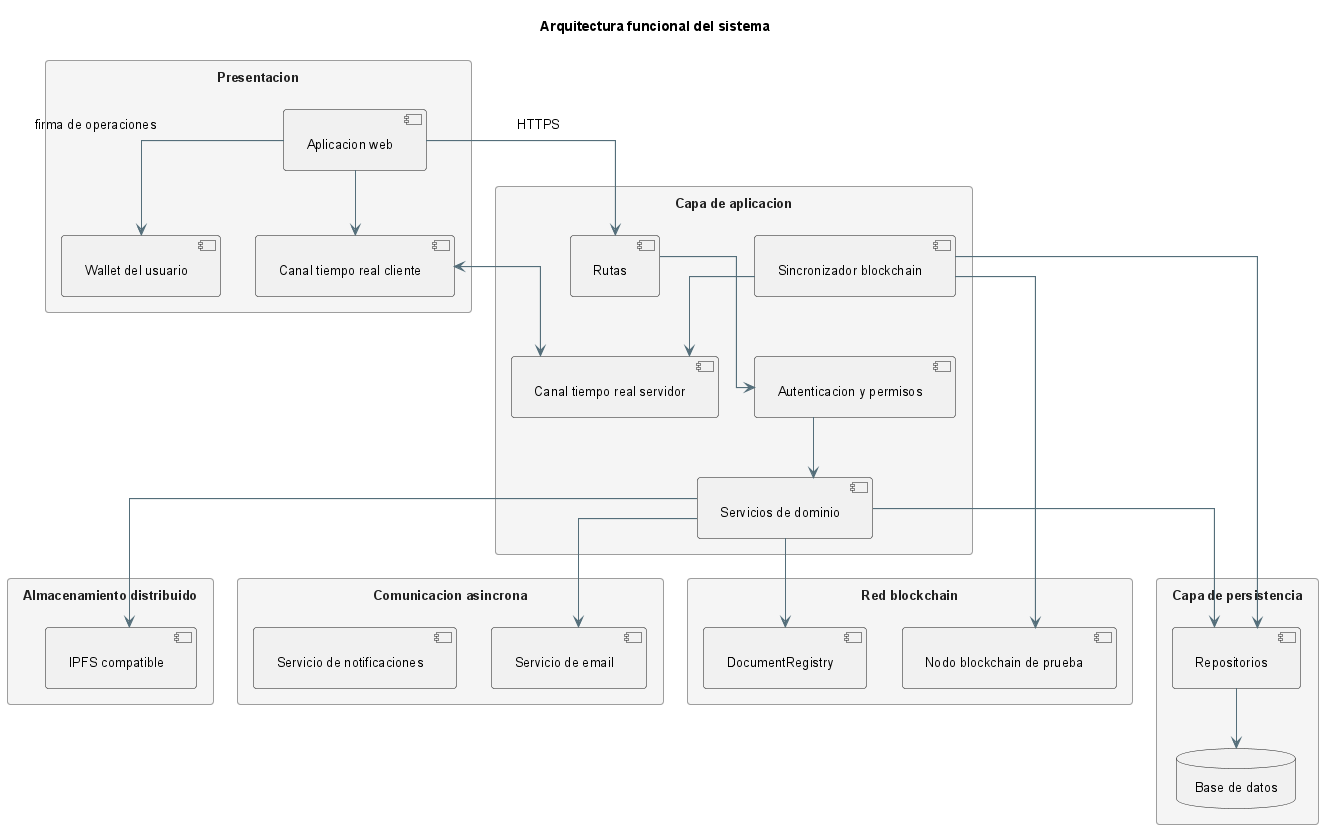
\includegraphics[width=\linewidth,height=0.82\textheight,keepaspectratio]{diagramas/arquitectura.png}
    \caption{Arquitectura del sistema DocumentChain por paquetes funcionales}
    \label{fig:arquitectura}
\end{figure}
\end{landscape}
\clearpage

\section{Glosario}

\begin{description}
    \item[AES-256-GCM] Advanced Encryption Standard con modo Galois/Counter Mode, algoritmo de cifrado simétrico.
    \item[Argon2id] Función de derivación de claves resistente a ataques de fuerza bruta.
    \item[Blockchain] Registro distribuido e inmutable de transacciones.
    \item[CID] Content Identifier, identificador único de contenido en IPFS basado en hash criptográfico.
    \item[CUID] Collision-resistant Unique Identifier, generador de IDs únicos.
    \item[RSA-OAEP] Esquema de cifrado asimétrico utilizado para proteger claves simétricas de documentos privados.
    \item[EIP-191] Ethereum Improvement Proposal para firmas de mensajes estándar.
    \item[Event Listener] Servicio que escucha eventos emitidos por smart contracts.
    \item[IPFS] InterPlanetary File System, sistema de archivos distribuido peer-to-peer.
    \item[JWT] JSON Web Token, estándar de token de autenticación.
    \item[OpenZeppelin] Biblioteca de smart contracts seguros y auditados.
    \item[Pinning] Mantener contenido permanentemente disponible en IPFS.
    \item[Prisma] ORM moderno para TypeScript y Node.js.
    \item[Re-encriptación] Proceso de cambiar el cifrado de una clave sin exponer el contenido.
    \item[Smart Contract] Programa auto-ejecutable desplegado en blockchain.
    \item[TOTP] Time-based One-Time Password, para autenticación de dos factores.
    \item[TxHash] Transaction Hash, identificador único de transacción blockchain.
    \item[Wallet] Monedero de criptomonedas con clave privada para firmar transacciones.
    \item[PublicId] Identificador público corto que permite resolver un documento publicado mediante enlace o código QR.
\end{description}

\section*{Bibliografía}
\addcontentsline{toc}{section}{Bibliografía}

\begin{enumerate}
    \item Durán, A., \& Bernárdez, B. (2000). \textit{A Requirements Elicitation Approach Based in Templates and Patterns}. Universidad de Sevilla.
    \item NIST. (2001). \textit{FIPS 197: Advanced Encryption Standard (AES)}. National Institute of Standards and Technology.
    \item NIST. (2020). \textit{FIPS 186-5: Digital Signature Standard (DSS)}. National Institute of Standards and Technology.
    \item OWASP Foundation. (2021). \textit{OWASP Top 10: 2021}. \url{https://owasp.org/Top10/}
    \item OpenZeppelin. (2025). \textit{OpenZeppelin Contracts Documentation}. \url{https://docs.openzeppelin.com/}
    \item Ethereum Foundation. (2025). \textit{Ethereum Developer Documentation}. \url{https://ethereum.org/en/developers/docs/}
    \item Protocol Labs. (2025). \textit{IPFS Documentation}. \url{https://docs.ipfs.tech/}
    \item Prisma. (2025). \textit{Prisma ORM Documentation}. \url{https://www.prisma.io/docs}
\end{enumerate}

\end{document}
